%=====================================================================
% CUADERNO DE COMPUTACIÓN CUÁNTICA
% Pensado para imprimir a doble cara y encuadernar: los capítulos y las
% secciones empiezan siempre en una página derecha (impar), y las páginas
% que quedan en blanco para conseguirlo no llevan cabecera ni número.
%=====================================================================
\documentclass[11pt, a4paper, twoside, openright]{report}

% --- Idioma y codificación ---
\usepackage[utf8]{inputenc}
\usepackage[T1]{fontenc}
\usepackage[spanish, es-noshorthands, es-tabla]{babel}

% --- Márgenes: margen extra en el lado del lomo para encuadernar ---
\usepackage[a4paper, top=2.5cm, bottom=2.5cm, inner=3cm, outer=2cm, bindingoffset=0.5cm]{geometry}

% --- Matemáticas, figuras, color, código ---
\usepackage{amsmath, amssymb, amsthm}
\usepackage{graphicx}
\usepackage{xcolor}
\usepackage{listings}
\usepackage[breakable]{tcolorbox}
\tcbset{breakable}

% --- Circuitos cuánticos ---
\usepackage{tikz}
\usetikzlibrary{quantikz2}

% --- Páginas en blanco sin cabecera ni número ---
\usepackage{emptypage}

% --- Cabeceras: capítulo en páginas pares, sección en impares ---
\usepackage{fancyhdr}
\pagestyle{fancy}
\fancyhf{}
\fancyhead[LE]{\small\nouppercase{\leftmark}}
\fancyhead[RO]{\small\nouppercase{\rightmark}}
\fancyfoot[LE,RO]{\thepage}
\renewcommand{\headrulewidth}{0.4pt}
\setlength{\headheight}{14pt}

% --- Configuración del código Python ---
\lstset{
    language=Python,
    basicstyle=\small\ttfamily,
    backgroundcolor=\color{gray!10},
    frame=single,
    rulecolor=\color{black!30},
    keywordstyle=\color{blue}\bfseries,
    commentstyle=\color{green!50!black}\itshape,
    stringstyle=\color{orange},
    showstringspaces=false,
    breaklines=true,
    inputencoding=utf8,
    extendedchars=true,
    literate={á}{{\'a}}1 {é}{{\'e}}1 {í}{{\'i}}1 {ó}{{\'o}}1 {ú}{{\'u}}1 {ñ}{{\~n}}1 {Á}{{\'A}}1 {É}{{\'E}}1 {Í}{{\'I}}1 {Ó}{{\'O}}1 {Ú}{{\'U}}1 {Ñ}{{\~N}}1 {¿}{{?`}}1 {⊗}{{$\otimes$}}1 {⟩}{{$\rangle$}}1 {√}{{$\surd$}}1 {·}{{$\cdot$}}1
}

% --- Enlaces (se carga el último) ---
\usepackage{hyperref}
\hypersetup{colorlinks=true, linkcolor=blue, urlcolor=cyan, citecolor=teal,
            pdftitle={Cuaderno de Computación Cuántica}}

\begin{document}

% =========================== PORTADA ================================
\begin{titlepage}
\centering
\vspace*{4cm}
{\Huge\bfseries Cuaderno de Computación Cuántica\par}
\vspace{1cm}
{\Large Fundamentos de información cuántica\par}
\vspace{2cm}
{\large Notas de estudio sobre el curso \textit{Understanding Quantum Information and Computation} (IBM Quantum, John Watrous)\par}
\vfill
{\large Elia Torres Simón\par}
\vspace{0.5cm}
{\large Trabajo de Fin de Grado --- Grado en Matemáticas, UCM\par}
\vspace{0.5cm}
{\large \today\par}
\end{titlepage}

% ========================== PRESENTACIÓN ============================
\cleardoublepage
\thispagestyle{empty}
\section*{Sobre este cuaderno}

\noindent Este cuaderno recoge, de forma autocontenida, los fundamentos de información cuántica necesarios para el Trabajo de Fin de Grado sobre métodos de kernel cuánticos. Sigue el curso \textit{Understanding Quantum Information and Computation} de IBM Quantum \cite{watrous2024understanding}, ampliado con demostraciones y explicaciones de todo lo que va más allá del álgebra lineal básica.

\noindent Cada capítulo tiene la misma estructura:
\begin{itemize}
    \item \textbf{Información clásica}, que sirve de punto de referencia y analogía.
    \item \textbf{Información cuántica}, con la teoría completa.
    \item \textbf{Implementación en Qiskit}, donde se comprueban numéricamente los resultados.
    \item \textbf{Resumen: un ejemplo guiado}, que recorre todos los conceptos con una sola historia y números concretos. Puede leerse antes de la teoría como introducción, o después como repaso.
\end{itemize}

\noindent \textbf{Código de colores de las cajas:}
\begin{itemize}
    \item \colorbox{teal!10}{Verde azulado}: definiciones, proposiciones y notas teóricas.
    \item \colorbox{gray!10}{Gris}: demostraciones y pasos de los ejemplos guiados.
    \item \colorbox{blue!8}{Azul}: notas aclaratorias e intuición.
    \item \colorbox{cyan!10}{Cian}: ejemplos.
\end{itemize}

\noindent Las cajas de \textbf{Conexión con el TFG} señalan los resultados que se usarán directamente en el estudio de los kernels cuánticos.

% ============================ ÍNDICE ================================
\cleardoublepage
\tableofcontents


\chapter{Sistemas individuales}

\noindent En este capítulo se estudia la información de un \textbf{único sistema}: primero la información clásica (estados probabilísticos y matrices estocásticas) y después la cuántica (vectores de estado y matrices unitarias). Veremos que ambas tienen la misma estructura matemática, y que toda la diferencia procede de dos cambios aparentemente pequeños: las entradas pasan a ser números complejos, y la normalización pasa a hacerse con módulos al cuadrado.

\begin{tcolorbox}[colback=teal!5!white,colframe=teal!75!black,title=\textbf{Nota Teórica: Dos descripciones de la información cuántica}]
La información cuántica admite dos descripciones matemáticas:

\textbf{Descripción simplificada} (la de este cuaderno): los estados cuánticos se representan mediante \textbf{vectores} de norma $1$ y las operaciones mediante \textbf{matrices unitarias}. Es la más sencilla, la que suele aprenderse primero, y basta para entender la mayoría de los algoritmos cuánticos.

\textbf{Descripción general}: los estados se representan mediante \textbf{matrices densidad}, es decir, matrices $\rho$ semidefinidas positivas y de traza $1$. Permite una clase más amplia de mediciones y operaciones, e incluye como casos particulares:
\begin{itemize}
    \item la descripción simplificada: al vector $|\psi\rangle$ le corresponde la matriz $\rho = |\psi\rangle\langle\psi|$;
    \item la información clásica: al vector de probabilidad $u$ le corresponde la matriz diagonal $\rho = \mathrm{diag}(u)$.
\end{itemize}
Una ventaja de las matrices densidad es que eliminan la fase global: $e^{i\theta}|\psi\rangle$ y $|\psi\rangle$ dan la misma matriz, pues $\left(e^{i\theta}|\psi\rangle\right)\left(e^{i\theta}|\psi\rangle\right)^\dagger = e^{i\theta}e^{-i\theta}|\psi\rangle\langle\psi| = |\psi\rangle\langle\psi|$.

\textbf{Conexión con el TFG:} Havlíček et al.\ \cite{havlicek2019supervised} describen los datos codificados como $|\Phi(\vec x)\rangle\langle\Phi(\vec x)|$, y el kernel cuántico se escribe como $K(\mathbf{x},\mathbf{y}) = \mathrm{Tr}\big[\rho(\mathbf{x})\rho(\mathbf{y})\big]$. Por eso la descripción general aparecerá al estudiar los kernels cuánticos.
\end{tcolorbox}
\cleardoublepage
\section{Información Clásica}

\noindent Antes de describir la información cuántica conviene estudiar la información clásica, por tres motivos. Primero, aunque ambas difieren en aspectos llamativos, sus descripciones matemáticas son muy parecidas: en los dos casos los estados son vectores y las operaciones son matrices. Segundo, la información clásica proporciona un punto de referencia familiar y una fuente de analogías que llega sorprendentemente lejos: muchas preguntas sobre información cuántica tienen un análogo clásico cuya respuesta es sencilla y aclara la pregunta original. Tercero, en esta sección se introduce la \textbf{notación de Dirac}, que se usará en todo el trabajo y que no es exclusiva de la mecánica cuántica: sirve para describir vectores y matrices en cualquier contexto.

\subsection{Estados clásicos}

\noindent Consideramos un \textbf{sistema}: una abstracción de un dispositivo o medio físico que almacena información. Suponemos que, en cada instante, el sistema se encuentra en uno de un número finito de \textbf{estados clásicos}, entendidos de forma intuitiva como configuraciones que pueden reconocerse y describirse sin ambigüedad.

\noindent Denotaremos el sistema por $\mathsf{X}$ y su conjunto de estados clásicos por $\Sigma$. Matemáticamente, la especificación de $\Sigma$ es el punto de partida: \textit{definimos} un bit como un sistema cuyo conjunto de estados clásicos es $\{0,1\}$. Supondremos siempre que $\Sigma$ es \textbf{finito y no vacío}: no tiene sentido físico un sistema sin estados, y aunque existen sistemas con infinitos estados clásicos, no los necesitaremos. En adelante, llamaremos \textit{conjunto de estados clásicos} a cualquier conjunto finito y no vacío.

\noindent Algunos ejemplos:
\begin{itemize}
    \item Si $\mathsf{X}$ es un \textbf{bit}, $\Sigma = \{0, 1\}$, llamado \textit{alfabeto binario}. Es el ejemplo al que volveremos constantemente.
    \item Si $\mathsf{X}$ es un dado de seis caras, $\Sigma = \{1, 2, 3, 4, 5, 6\}$.
    \item Si $\mathsf{X}$ es una base nucleica de una cadena de ADN, $\Sigma = \{A, C, G, T\}$.
    \item Si $\mathsf{X}$ es el interruptor de un ventilador, \\ $\Sigma = \{\text{alto}, \text{medio}, \text{bajo}, \text{apagado}\}$.
\end{itemize}

\subsection{Estados probabilísticos y vectores de probabilidad}

\noindent A veces conocemos con certeza el estado clásico de un sistema (sabemos que el ventilador está en \textit{alto}). Pero a menudo nuestro conocimiento es incierto, y lo describimos asociando una \textbf{probabilidad} a cada estado clásico posible. Esto es un \textbf{estado probabilístico}. Por ejemplo, si $\mathsf{X}$ es un bit y, por lo que sabemos de su historia, creemos que está en $0$ con probabilidad $3/4$ y en $1$ con probabilidad $1/4$, escribimos
\[ \Pr(\mathsf{X} = 0) = \frac{3}{4}, \qquad \Pr(\mathsf{X} = 1) = \frac{1}{4}, \]
o, de forma más compacta, mediante el vector columna
\[ \begin{pmatrix} 3/4 \\ 1/4 \end{pmatrix}, \]
donde, siguiendo el orden natural de $\{0,1\}$, la probabilidad de $0$ ocupa la primera entrada y la de $1$ la segunda.

\begin{tcolorbox}[colback=teal!5!white,colframe=teal!75!black,title=\textbf{Nota Teórica: Vectores indexados por un conjunto}]
En álgebra lineal básica los vectores de $\mathbb{R}^n$ tienen sus entradas numeradas por $1, 2, \dots, n$. Aquí resulta más natural numerarlas por los propios estados clásicos: la entrada ``$0$'', la entrada ``$1$'', la entrada ``alto''\dots

Formalmente, dado un conjunto finito $\Sigma$, se define
\[ \mathbb{R}^{\Sigma} = \{\, u : \Sigma \to \mathbb{R} \,\}, \]
el conjunto de todas las funciones de $\Sigma$ en $\mathbb{R}$, con la suma y el producto por escalares definidos punto a punto. Un elemento $u \in \mathbb{R}^\Sigma$ asigna a cada estado $a \in \Sigma$ un número $u(a)$, que escribiremos $u_a$ y llamaremos \textit{entrada $a$} de $u$. Es un espacio vectorial de dimensión $|\Sigma|$.

Si fijamos un orden en $\Sigma$, digamos $\Sigma = \{a_1, \dots, a_n\}$, la aplicación $u \mapsto (u_{a_1}, \dots, u_{a_n})^T$ es un isomorfismo $\mathbb{R}^\Sigma \cong \mathbb{R}^n$. Es decir, un vector de $\mathbb{R}^\Sigma$ ``es'' un vector columna de $\mathbb{R}^n$, una vez decidido en qué orden se escriben las entradas. El orden es arbitrario, pero suele haber uno natural (por ejemplo, $0$ antes que $1$).

Del mismo modo, una matriz con filas y columnas indexadas por $\Sigma$ es una familia de números $(M_{ba})_{b, a \in \Sigma}$, donde $b$ indica la fila y $a$ la columna.
\end{tcolorbox}

\begin{tcolorbox}[colback=teal!5!white,colframe=teal!75!black,title=\textbf{Definición: Vector de probabilidad}]
Un vector $u \in \mathbb{R}^\Sigma$ es un \textbf{vector de probabilidad} si
\begin{enumerate}
    \item todas sus entradas son no negativas: $u_a \geq 0$ para todo $a \in \Sigma$, y
    \item sus entradas suman uno: $\displaystyle\sum_{a \in \Sigma} u_a = 1$.
\end{enumerate}
Todo estado probabilístico de un sistema con conjunto de estados clásicos $\Sigma$ se representa mediante un vector de probabilidad, y recíprocamente, todo vector de probabilidad representa un estado probabilístico.
\end{tcolorbox}

\begin{tcolorbox}[colback=blue!5!white,colframe=blue!75!black,title=\textbf{Nota Aclaratoria: La geometría de los vectores de probabilidad}]
El conjunto de vectores de probabilidad de $\mathbb{R}^\Sigma$ se llama \textbf{símplex de probabilidad}. Para un bit es el segmento que une $(1,0)^T$ y $(0,1)^T$ en el plano; para un sistema con tres estados, el triángulo de vértices $(1,0,0)^T$, $(0,1,0)^T$ y $(0,0,1)^T$.

Es un conjunto \textbf{convexo}: si $u$ y $v$ son vectores de probabilidad y $t \in [0,1]$, entonces $tu + (1-t)v$ también lo es (sus entradas siguen siendo no negativas y siguen sumando uno). Interpretación: si con probabilidad $t$ el sistema está en el estado $u$ y con probabilidad $1-t$ en el estado $v$, el estado resultante es la ``mezcla'' $tu + (1-t)v$.

La ventaja de representar los estados como vectores, además de la notación compacta, es que las \textbf{operaciones} sobre estados probabilísticos se representarán como \textbf{productos matriz-vector}, como veremos enseguida.
\end{tcolorbox}

\subsection{Medición de estados probabilísticos}

\noindent Por \textbf{medir} un sistema entendemos observarlo y reconocer sin ambigüedad el estado clásico en que se encuentra. Nunca ``vemos'' un estado probabilístico: al mirar, solo vemos uno de los estados clásicos posibles. Si el sistema está en el estado probabilístico $u$, obtenemos el resultado $a \in \Sigma$ con probabilidad $u_a$.

\noindent Tras medir, nuestro conocimiento cambia. Si hemos reconocido que $\mathsf{X}$ está en el estado $a$, el nuevo vector de probabilidad que describe lo que sabemos es el que tiene un $1$ en la entrada $a$ y $0$ en todas las demás: indica que $\mathsf{X}$ está en $a$ con certeza. Denotamos este vector por
\[ |a\rangle \qquad (\text{se lee ``ket } a\text{''}), \]
y a los vectores de esta forma los llamamos \textbf{vectores de la base estándar}. Para un bit:
\[ |0\rangle = \begin{pmatrix} 1 \\ 0 \end{pmatrix}, \qquad |1\rangle = \begin{pmatrix} 0 \\ 1 \end{pmatrix}. \]

\noindent Los vectores $\{|a\rangle : a \in \Sigma\}$ forman la base canónica de $\mathbb{R}^\Sigma$, así que todo vector se escribe de forma única como combinación lineal de ellos:
\[ u = \sum_{a \in \Sigma} u_a\, |a\rangle, \qquad \text{por ejemplo,} \quad \begin{pmatrix} 3/4 \\ 1/4 \end{pmatrix} = \frac{3}{4}\,|0\rangle + \frac{1}{4}\,|1\rangle. \]
A menudo escribiremos los vectores precisamente de esta manera.

\begin{tcolorbox}[colback=cyan!5!white,colframe=cyan!75!black,title=\textbf{Ejemplo: La moneda tapada}]
Lanzamos una moneda equilibrada y la tapamos antes de mirarla. Con $\Sigma = \{\text{cara}, \text{cruz}\}$, en este orden, su estado probabilístico es
\[ \begin{pmatrix} 1/2 \\ 1/2 \end{pmatrix} = \frac{1}{2}\,|\text{cara}\rangle + \frac{1}{2}\,|\text{cruz}\rangle, \qquad |\text{cara}\rangle = \begin{pmatrix} 1 \\ 0 \end{pmatrix}, \quad |\text{cruz}\rangle = \begin{pmatrix} 0 \\ 1 \end{pmatrix}. \]
Si la destapamos y vemos cruz, actualizamos nuestra descripción a $|\text{cruz}\rangle$. Si volvemos a taparla y destaparla, seguirá siendo cruz, lo cual es coherente con el vector $|\text{cruz}\rangle$.

Esto parece trivial, y lo es. Pero los sistemas cuánticos se comportan de forma análoga al medirlos, y tener presente la versión clásica hace que la medición cuántica parezca mucho menos extraña.
\end{tcolorbox}

\begin{tcolorbox}[colback=blue!5!white,colframe=blue!75!black,title=\textbf{Aclaración: El cambio de estado tras la medición}]
Un estado probabilístico describe nuestro \textbf{conocimiento} sobre el sistema, no necesariamente algo físico. En el caso de la moneda, mirar no cambia la moneda: ya era cruz debajo de la mano. Lo que cambia es nuestra información, y con ella el vector, que pasa de $\frac{1}{2}|\text{cara}\rangle + \frac{1}{2}|\text{cruz}\rangle$ a $|\text{cruz}\rangle$. Otra persona que no haya mirado seguiría describiendo la moneda con el vector original, y no hay contradicción: personas con distinta información describen el mismo sistema con vectores distintos.

\textbf{El salto a la cuántica:} en el caso cuántico, la regla de actualización tras medir es formalmente la misma: el estado pasa a ser $|a\rangle$. La diferencia está en que las amplitudes cuánticas \textbf{no pueden interpretarse} simplemente como probabilidades que reflejan nuestra ignorancia. Son números complejos que, al aplicar operaciones, pueden \textbf{interferir}: sumarse o cancelarse entre sí. Las probabilidades clásicas, al ser no negativas, nunca se cancelan. Este fenómeno de interferencia, que veremos con operaciones como la de Hadamard, no tiene análogo clásico.
\end{tcolorbox}

\subsection{Operaciones deterministas}

\noindent La operación más sencilla sobre un sistema clásico es una \textbf{operación determinista}: cada estado clásico $a \in \Sigma$ se transforma en $f(a)$ mediante una función $f : \Sigma \to \Sigma$, sin intervención del azar. Como $\Sigma$ es finito, hay exactamente $|\Sigma|^{|\Sigma|}$ operaciones deterministas (para cada uno de los $|\Sigma|$ estados de entrada se elige uno de los $|\Sigma|$ posibles de salida).

\noindent Para un bit hay $2^2 = 4$ funciones $f : \{0,1\} \to \{0,1\}$:
\[
\begin{array}{c|c} a & f_1(a) \\ \hline 0 & 0 \\ 1 & 0 \end{array}
\qquad
\begin{array}{c|c} a & f_2(a) \\ \hline 0 & 0 \\ 1 & 1 \end{array}
\qquad
\begin{array}{c|c} a & f_3(a) \\ \hline 0 & 1 \\ 1 & 0 \end{array}
\qquad
\begin{array}{c|c} a & f_4(a) \\ \hline 0 & 1 \\ 1 & 1 \end{array}
\]
\begin{itemize}
    \item $f_1$ y $f_4$ son \textbf{constantes}: $f_1(a) = 0$ y $f_4(a) = 1$ para todo $a$.
    \item $f_2$ y $f_3$ son \textbf{equilibradas}: cada valor de salida aparece el mismo número de veces al recorrer las entradas. $f_2$ es la \textbf{identidad} ($f_2(a) = a$) y $f_3$ es la negación o \textbf{NOT} ($f_3(0) = 1$, $f_3(1) = 0$).
\end{itemize}

\noindent La acción de una operación determinista sobre los estados probabilísticos se representa mediante una matriz.

\begin{tcolorbox}[colback=teal!5!white,colframe=teal!75!black,title=\textbf{Proposición: Matriz de una operación determinista}]
Para cada función $f : \Sigma \to \Sigma$ existe una única matriz $M$ (con filas y columnas indexadas por $\Sigma$) tal que
\[ M\,|a\rangle = |f(a)\rangle \qquad \text{para todo } a \in \Sigma. \]
Sus entradas son $M_{ba} = 1$ si $b = f(a)$ y $M_{ba} = 0$ en otro caso. En particular, \textbf{cada columna de $M$ tiene exactamente un $1$} y el resto de entradas son $0$.
\end{tcolorbox}

\begin{tcolorbox}[colback=gray!5!white,colframe=gray!75!black,title=\textbf{Demostración}]
Es un hecho básico del álgebra lineal: una aplicación lineal queda determinada de forma única por las imágenes de los vectores de una base, y la columna $a$ de su matriz es precisamente la imagen del vector $|a\rangle$ (porque $M|a\rangle$ ``selecciona'' la columna $a$ de $M$). Imponer $M|a\rangle = |f(a)\rangle$ para todo $a$ equivale, por tanto, a fijar cada columna de $M$: la columna $a$ debe ser $|f(a)\rangle$, que tiene un $1$ en la fila $f(a)$ y ceros en el resto. Esto prueba la existencia, la unicidad y la forma de las entradas. \hfill $\square$
\end{tcolorbox}

\noindent Para las cuatro funciones anteriores, las matrices son
\[
M_1 = \begin{pmatrix} 1 & 1 \\ 0 & 0 \end{pmatrix}, \quad
M_2 = \begin{pmatrix} 1 & 0 \\ 0 & 1 \end{pmatrix}, \quad
M_3 = \begin{pmatrix} 0 & 1 \\ 1 & 0 \end{pmatrix}, \quad
M_4 = \begin{pmatrix} 0 & 0 \\ 1 & 1 \end{pmatrix}.
\]
Por ejemplo, para $M_1$:
\begin{align*}
M_1|0\rangle &= \begin{pmatrix} 1 & 1 \\ 0 & 0 \end{pmatrix}\begin{pmatrix} 1 \\ 0 \end{pmatrix} = \begin{pmatrix} 1 \\ 0 \end{pmatrix} = |0\rangle = |f_1(0)\rangle, \\
M_1|1\rangle &= \begin{pmatrix} 1 & 1 \\ 0 & 0 \end{pmatrix}\begin{pmatrix} 0 \\ 1 \end{pmatrix} = \begin{pmatrix} 1 \\ 0 \end{pmatrix} = |0\rangle = |f_1(1)\rangle.
\end{align*}
Las otras tres se comprueban igual. Nótese que $M_3$ coincide con la matriz de Pauli $X$ que aparecerá en el caso cuántico.

\begin{tcolorbox}[colback=blue!5!white,colframe=blue!75!black,title=\textbf{Nota Aclaratoria: Operaciones que pierden información}]
La matriz $M_f$ es invertible si y solo si $f$ es biyectiva. En ese caso $M_f$ es una \textbf{matriz de permutación} (un $1$ en cada fila y en cada columna), y la operación puede deshacerse aplicando la de $f^{-1}$. Por ejemplo, $M_3$ (NOT) es su propia inversa: $M_3^2 = I$.

En cambio, las funciones constantes \textbf{pierden información}: tras aplicar $f_1$, el bit vale $0$ tanto si antes era $0$ como si era $1$, y no hay forma de saber cuál era. Algebraicamente, $M_1$ tiene determinante $0$.

Esta distinción será importante: en el caso cuántico, las operaciones sobre un sistema aislado son matrices unitarias, que son \textbf{siempre invertibles}. Las operaciones cuánticas (unitarias) son, por tanto, reversibles, mientras que las clásicas en general no lo son; la medición, en cambio, no es reversible.
\end{tcolorbox}

\subsection{Notación de Dirac}

\noindent Hemos escrito los vectores columna de la base estándar como $|a\rangle$. De forma análoga, denotamos por
\[ \langle a| \qquad (\text{se lee ``bra } a\text{''}) \]
el \textbf{vector fila} con un $1$ en la entrada $a$ y $0$ en las demás. Para un bit:
\[ \langle 0| = \begin{pmatrix} 1 & 0 \end{pmatrix}, \qquad \langle 1| = \begin{pmatrix} 0 & 1 \end{pmatrix}. \]
Es decir, $\langle a|$ es la transpuesta de $|a\rangle$. Viendo bras y kets como matrices ($1 \times |\Sigma|$ y $|\Sigma| \times 1$, respectivamente), podemos multiplicarlos en los dos órdenes posibles, y cada orden da algo muy distinto.

\begin{tcolorbox}[colback=teal!5!white,colframe=teal!75!black,title=\textbf{Definición: Producto bra-ket (producto interno) y producto ket-bra (producto exterior)}]
\textbf{Bra por ket} (fila por columna): $\langle a| \cdot |b\rangle$ es una matriz $1 \times 1$, es decir, un \textbf{número}. Se escribe abreviadamente $\langle a | b \rangle$ (``bracket'') y vale
\[ \langle a | b \rangle = \begin{cases} 1 & \text{si } a = b, \\ 0 & \text{si } a \neq b. \end{cases} \]
Es el \textbf{producto escalar} (o producto interno) de $|a\rangle$ y $|b\rangle$; la fórmula anterior dice que la base estándar es ortonormal.

\textbf{Ket por bra} (columna por fila): $|b\rangle \cdot \langle a|$, escrito $|b\rangle\langle a|$, es una \textbf{matriz cuadrada} $|\Sigma| \times |\Sigma|$, llamada \textbf{producto exterior}. Tiene un $1$ en la posición (fila $b$, columna $a$) y $0$ en todas las demás. Por ejemplo:
\[ |0\rangle\langle 1| = \begin{pmatrix} 1 \\ 0 \end{pmatrix}\begin{pmatrix} 0 & 1 \end{pmatrix} = \begin{pmatrix} 0 & 1 \\ 0 & 0 \end{pmatrix}. \]
Las matrices $|b\rangle\langle a|$ son las \textbf{matrices elementales} (a veces denotadas $E_{ba}$), que forman una base del espacio de matrices. Por tanto, \textbf{cualquier matriz} se escribe como
\[ M = \sum_{a, b \in \Sigma} M_{ba}\; |b\rangle\langle a|. \]
\end{tcolorbox}

\noindent El nombre de la notación viene de aquí: un \textit{bra} $\langle a|$ junto a un \textit{ket} $|b\rangle$ forman un \textit{bracket} $\langle a|b\rangle$ (``corchete'', en inglés). Se debe al físico Paul Dirac y se conoce como \textbf{notación de Dirac}. Su gran ventaja es que la asociatividad del producto de matrices permite manipular expresiones casi ``automáticamente'', como muestra el siguiente resultado.

\begin{tcolorbox}[colback=teal!5!white,colframe=teal!75!black,title=\textbf{Proposición: Operaciones deterministas en notación de Dirac}]
La matriz de la operación determinista asociada a $f : \Sigma \to \Sigma$ es
\[ M = \sum_{a \in \Sigma} |f(a)\rangle\langle a|. \]
\end{tcolorbox}

\begin{tcolorbox}[colback=gray!5!white,colframe=gray!75!black,title=\textbf{Demostración}]
Basta comprobar que esta matriz cumple $M|b\rangle = |f(b)\rangle$ para todo $b \in \Sigma$, ya que por la proposición anterior esa condición la determina. Usando la linealidad y la asociatividad del producto de matrices:
\[
M|b\rangle = \Big( \sum_{a \in \Sigma} |f(a)\rangle\langle a| \Big) |b\rangle = \sum_{a \in \Sigma} |f(a)\rangle \, \langle a|b\rangle = |f(b)\rangle,
\]
porque $\langle a|b\rangle = 0$ salvo para $a = b$, en cuyo caso vale $1$: de toda la suma solo sobrevive el término $a = b$. \hfill $\square$
\end{tcolorbox}

\noindent Por ejemplo, para la función constante $f_4$:
\[
M_4 = |f_4(0)\rangle\langle 0| + |f_4(1)\rangle\langle 1| = |1\rangle\langle 0| + |1\rangle\langle 1|
= \begin{pmatrix} 0 & 0 \\ 1 & 0 \end{pmatrix} + \begin{pmatrix} 0 & 0 \\ 0 & 1 \end{pmatrix}
= \begin{pmatrix} 0 & 0 \\ 1 & 1 \end{pmatrix}.
\]

\noindent El producto $\langle a|b\rangle$ es un caso particular del \textbf{producto interno}, que tendrá un papel central en la información cuántica. En el caso cuántico, para vectores con entradas complejas, el \textit{bra} de un vector será su \textit{transpuesta conjugada}, no solo su transpuesta (Sección 1.2). Y es precisamente a partir de un producto interno entre estados cuánticos (en concreto, de su módulo al cuadrado) como se definirá el kernel cuántico de este trabajo.

\subsection{Operaciones probabilísticas y matrices estocásticas}

\noindent Además de las deterministas, hay \textbf{operaciones probabilísticas}, en las que interviene el azar. Por ejemplo, sobre un bit: si el estado es $0$, se deja igual; si es $1$, se ``lanza una moneda'', de modo que pasa a $0$ con probabilidad $1/2$ y se queda en $1$ con probabilidad $1/2$. Esta operación se representa mediante la matriz
\[ M = \begin{pmatrix} 1 & 1/2 \\ 0 & 1/2 \end{pmatrix}. \]
En efecto, $M|0\rangle = |0\rangle$ y $M|1\rangle = \frac{1}{2}|0\rangle + \frac{1}{2}|1\rangle$. En general, la \textbf{columna $a$} de la matriz es el \textbf{estado probabilístico que se obtiene si la entrada es el estado clásico $a$}.

\begin{tcolorbox}[colback=teal!5!white,colframe=teal!75!black,title=\textbf{Definición: Matriz estocástica}]
Una matriz cuadrada $M$ (con filas y columnas indexadas por $\Sigma$) es \textbf{estocástica} si
\begin{enumerate}
    \item todas sus entradas son reales y no negativas: $M_{ba} \geq 0$, y
    \item cada columna suma uno: $\displaystyle\sum_{b \in \Sigma} M_{ba} = 1$ para todo $a \in \Sigma$.
\end{enumerate}
Equivalentemente, $M$ es estocástica si y solo si \textbf{todas sus columnas son vectores de probabilidad}. Las operaciones probabilísticas sobre un sistema son exactamente las representadas por matrices estocásticas.

\textit{Observación:} la condición 2 se escribe de forma compacta como $\mathbf{1}^T M = \mathbf{1}^T$, donde $\mathbf{1}$ es el vector con todas las entradas iguales a $1$: la entrada $a$ del vector fila $\mathbf{1}^T M$ es precisamente la suma de la columna $a$.
\end{tcolorbox}

\noindent Las matrices de las operaciones deterministas son un caso particular de matrices estocásticas (cada columna es un vector de la base estándar, que es un vector de probabilidad).

\noindent La caracterización más importante de las matrices estocásticas es que son exactamente las que ``respetan'' los estados probabilísticos.

\begin{tcolorbox}[colback=teal!5!white,colframe=teal!75!black,title=\textbf{Proposición: Caracterización de las matrices estocásticas}]
Una matriz $M$ es estocástica si y solo si transforma todo vector de probabilidad en un vector de probabilidad.
\end{tcolorbox}

\begin{tcolorbox}[colback=gray!5!white,colframe=gray!75!black,title=\textbf{Demostración}]
($\Rightarrow$) Sean $M$ estocástica y $u$ un vector de probabilidad. Cada entrada de $Mu$ es $(Mu)_b = \sum_{a} M_{ba} u_a$, suma de productos de números no negativos, luego $(Mu)_b \geq 0$. Además, intercambiando el orden de las sumas,
\[ \sum_{b \in \Sigma} (Mu)_b = \sum_{b}\sum_{a} M_{ba}\, u_a = \sum_{a} u_a \Big( \sum_{b} M_{ba} \Big) = \sum_{a} u_a \cdot 1 = 1. \]

($\Leftarrow$) Supongamos que $M$ transforma vectores de probabilidad en vectores de probabilidad. Cada $|a\rangle$ es un vector de probabilidad, luego $M|a\rangle$, que es la columna $a$ de $M$, también lo es. Como esto vale para todas las columnas, $M$ es estocástica. \hfill $\square$
\end{tcolorbox}

\noindent Otra forma de entender las operaciones probabilísticas es como \textbf{elecciones al azar de operaciones deterministas}. La operación del ejemplo equivale a aplicar la identidad o la función constante $0$, cada una con probabilidad $1/2$:
\[
\begin{pmatrix} 1 & 1/2 \\ 0 & 1/2 \end{pmatrix} = \frac{1}{2}\begin{pmatrix} 1 & 0 \\ 0 & 1 \end{pmatrix} + \frac{1}{2}\begin{pmatrix} 1 & 1 \\ 0 & 0 \end{pmatrix} = \frac12 M_2 + \frac12 M_1.
\]
Esto no es una casualidad del ejemplo, sino un hecho general.

\begin{tcolorbox}[colback=teal!5!white,colframe=teal!75!black,title=\textbf{Proposición: Las operaciones probabilísticas son mezclas de deterministas}]
Toda matriz estocástica $M$ es una \textbf{combinación convexa} de matrices de operaciones deterministas: existen probabilidades $p(f) \geq 0$, con $\sum_f p(f) = 1$, tales que
\[ M = \sum_{f : \Sigma \to \Sigma} p(f)\, M_f, \]
donde $M_f$ es la matriz de la operación determinista asociada a $f$.
\end{tcolorbox}

\begin{tcolorbox}[colback=gray!5!white,colframe=gray!75!black,title=\textbf{Demostración}]
La idea es elegir la imagen de cada estado de forma independiente, usando la columna correspondiente de $M$ como distribución de probabilidad. Definimos, para cada $f : \Sigma \to \Sigma$,
\[ p(f) = \prod_{a \in \Sigma} M_{f(a)\,a}. \]
Claramente $p(f) \geq 0$. Elegir una función $f$ es lo mismo que elegir, de forma independiente para cada $a \in \Sigma$, un valor $f(a) \in \Sigma$; por tanto, al sumar sobre todas las $f$ el producto se factoriza:
\[ \sum_{f} p(f) = \prod_{a \in \Sigma} \Big( \sum_{b \in \Sigma} M_{ba} \Big) = \prod_{a \in \Sigma} 1 = 1. \]
Veamos que $\sum_f p(f) M_f = M$ comparando la entrada $(b, a)$. La entrada $(b,a)$ de $M_f$ vale $1$ si $f(a) = b$ y $0$ en otro caso, luego
\[ \Big( \sum_f p(f) M_f \Big)_{ba} = \sum_{f \,:\, f(a) = b} p(f) = M_{ba} \prod_{a' \neq a} \Big( \sum_{b' \in \Sigma} M_{b'a'} \Big) = M_{ba}, \]
donde hemos fijado el factor correspondiente a $a$ (que vale $M_{ba}$) y hemos sumado libremente sobre los valores de $f$ en los demás estados. \hfill $\square$

\textit{Comprobación con el ejemplo:} $p(f) \neq 0$ exige $f(0) = 0$ (pues $M_{10} = 0$). Quedan $f_1$, con $p(f_1) = M_{00} M_{01} = 1 \cdot \frac12$, y $f_2$, con $p(f_2) = M_{00} M_{11} = 1 \cdot \frac12$. Es exactamente la descomposición anterior.
\end{tcolorbox}

\subsection{Composición de operaciones probabilísticas}

\noindent Sean $M_1, \dots, M_n$ matrices estocásticas que representan operaciones probabilísticas sobre $\mathsf{X}$. Si aplicamos $M_1$ al estado $u$, obtenemos $M_1 u$; si después aplicamos $M_2$, obtenemos
\[ M_2(M_1 u) = (M_2 M_1)\, u, \]
por la asociatividad del producto de matrices. Así, aplicar primero $M_1$ y después $M_2$ equivale a aplicar la única operación $M_2 M_1$. En general, aplicar $M_1, M_2, \dots, M_n$ en este orden (primero $M_1$, al final $M_n$) equivale a aplicar
\[ M_n \cdots M_2 M_1. \]
\textbf{Atención al orden}: la primera operación que se aplica es la que queda más a la derecha, porque es la que actúa primero sobre el vector.

\begin{tcolorbox}[colback=teal!5!white,colframe=teal!75!black,title=\textbf{Proposición: El producto de matrices estocásticas es estocástico}]
Si $M_1$ y $M_2$ son estocásticas, $M_2 M_1$ también lo es. Por inducción, cualquier producto finito de matrices estocásticas es estocástico.
\end{tcolorbox}

\begin{tcolorbox}[colback=gray!5!white,colframe=gray!75!black,title=\textbf{Demostración}]
Las entradas de $M_2 M_1$ son sumas de productos de números no negativos, luego son no negativas. Para las columnas, usando la observación $\mathbf{1}^T M = \mathbf{1}^T$:
\[ \mathbf{1}^T (M_2 M_1) = (\mathbf{1}^T M_2)\, M_1 = \mathbf{1}^T M_1 = \mathbf{1}^T. \]
(Alternativamente: $M_2 M_1$ transforma vectores de probabilidad en vectores de probabilidad, por ser composición de dos aplicaciones que lo hacen, y basta aplicar la caracterización anterior.) \hfill $\square$
\end{tcolorbox}

\noindent Aunque el producto de matrices es asociativo, \textbf{no es conmutativo}, así que el orden en que se aplican las operaciones importa. Por ejemplo, con la función constante $0$ y la negación,
\[
M_1 = \begin{pmatrix} 1 & 1 \\ 0 & 0 \end{pmatrix}, \qquad M_3 = \begin{pmatrix} 0 & 1 \\ 1 & 0 \end{pmatrix},
\]
se obtiene
\[
M_3 M_1 = \begin{pmatrix} 0 & 0 \\ 1 & 1 \end{pmatrix}, \qquad M_1 M_3 = \begin{pmatrix} 1 & 1 \\ 0 & 0 \end{pmatrix}.
\]
La interpretación es inmediata: poner el bit a $0$ y después negarlo deja siempre el bit en $1$ ($M_3 M_1$ es la constante $1$); negarlo y después ponerlo a $0$ deja siempre el bit en $0$ ($M_1 M_3$ es la constante $0$).

\cleardoublepage
\section{Información Cuántica}

\noindent Pasamos ahora a la información cuántica. Veremos que su descripción matemática es muy parecida a la de la información clásica: los estados siguen siendo vectores indexados por los estados clásicos del sistema y las operaciones siguen siendo matrices. Lo que cambia son dos cosas aparentemente pequeñas: las entradas pasan a ser \textbf{números complejos}, y la condición de normalización pasa de la \textbf{suma de las entradas} a la \textbf{suma de sus módulos al cuadrado}. Toda la diferencia entre información clásica y cuántica, incluida cualquier ventaja de un ordenador cuántico, procede en última instancia de estos dos cambios.

\begin{tcolorbox}[colback=teal!5!white,colframe=teal!75!black,title=\textbf{Repaso: Números complejos}]
Un número complejo es $z = x + iy$, con $x, y \in \mathbb{R}$ e $i^2 = -1$. Recordamos las nociones que se usarán constantemente:
\begin{itemize}
    \item \textbf{Conjugado:} $\overline{z} = x - iy$. Cumple $\overline{z + w} = \overline{z} + \overline{w}$ y $\overline{zw} = \overline{z}\,\overline{w}$.
    \item \textbf{Módulo:} $|z| = \sqrt{x^2 + y^2}$, que es la distancia de $z$ al origen en el plano complejo. Su cuadrado se calcula sin raíces como
    \[ |z|^2 = z\,\overline{z} = (x+iy)(x-iy) = x^2 + y^2. \]
    Es siempre un número real no negativo, y $|z|^2 = 0$ si y solo si $z = 0$. Además, $|zw| = |z|\,|w|$.
    \item \textbf{Forma polar y fórmula de Euler:} todo $z \neq 0$ se escribe como
    \[ z = r\, e^{i\theta}, \qquad r = |z| > 0, \qquad e^{i\theta} = \cos\theta + i \sin\theta. \]
    El ángulo $\theta$ se llama \textbf{argumento} o \textbf{fase} de $z$, y está determinado salvo múltiplos de $2\pi$. Los números $e^{i\theta}$ son exactamente los complejos de módulo $1$ (la circunferencia unidad), y se multiplican sumando fases: $e^{i\alpha}e^{i\beta} = e^{i(\alpha+\beta)}$.
    \item \textbf{Valores notables:} $e^{i\pi/2} = i$, \; $e^{i\pi} = -1$, \; $e^{i\pi/4} = \dfrac{1+i}{\sqrt{2}}$.
\end{itemize}
\textbf{Interpretación clave:} multiplicar un complejo por $e^{i\theta}$ lo \textbf{gira} un ángulo $\theta$ sin cambiar su módulo. Por eso, cambiar la fase de una amplitud no cambia su módulo, y veremos que tampoco cambia la probabilidad asociada; pero sí cambia cómo se suma con otras amplitudes.
\end{tcolorbox}

\subsection{Vectores de estado cuánticos}

\noindent El \textbf{estado cuántico} de un sistema se representa mediante un vector columna indexado, como antes, por los estados clásicos del sistema. Si $\Sigma$ es el conjunto de estados clásicos, el vector vive en $\mathbb{C}^\Sigma$, el análogo complejo de $\mathbb{R}^\Sigma$ (funciones $\Sigma \to \mathbb{C}$, o vectores columna de $\mathbb{C}^n$ una vez fijado un orden en $\Sigma$).

\begin{tcolorbox}[colback=teal!5!white,colframe=teal!75!black,title=\textbf{Definición: Vector de estado cuántico}]
Un vector $v \in \mathbb{C}^\Sigma$ es un \textbf{vector de estado cuántico} si
\begin{enumerate}
    \item sus entradas son \textbf{números complejos} (llamados \textbf{amplitudes}), y
    \item la suma de los \textbf{módulos al cuadrado} de sus entradas es $1$: $\displaystyle\sum_{a \in \Sigma} |v_a|^2 = 1$.
\end{enumerate}
\end{tcolorbox}

\noindent Comparado con los vectores de probabilidad, las entradas ya no tienen por qué ser reales ni no negativas, y lo que debe valer $1$ no es la suma de las entradas sino la de sus módulos al cuadrado. La segunda condición tiene una lectura geométrica: la \textbf{norma euclídea} de un vector $v = (\alpha_1, \dots, \alpha_n)^T \in \mathbb{C}^n$ es
\[ \|v\| = \sqrt{\sum_{k=1}^n |\alpha_k|^2}, \]
de modo que la condición 2 equivale a $\|v\| = 1$. Es decir: \textbf{los vectores de estado cuánticos son exactamente los vectores unitarios (de norma 1) de $\mathbb{C}^\Sigma$}. Nótese que en $\mathbb{C}^n$ la norma se define con $|\alpha_k|^2$ y no con $\alpha_k^2$: el cuadrado de un complejo puede ser negativo o incluso no real ($i^2 = -1$), y no serviría para medir longitudes.

\begin{tcolorbox}[colback=blue!5!white,colframe=blue!75!black,title=\textbf{Nota Aclaratoria: Comparación entre ambos tipos de estado}]
\begin{center}
\begin{tabular}{l|c|c}
 & \textbf{Estado probabilístico} & \textbf{Estado cuántico} \\ \hline
 Entradas & reales, $u_a \ge 0$ & complejas, $v_a \in \mathbb{C}$ \\
 Normalización & $\sum_a u_a = 1$ & $\sum_a |v_a|^2 = 1$ \\
 Conjunto de estados & símplex (convexo) & esfera unidad de $\mathbb{C}^\Sigma$ \\
 Operaciones & matrices estocásticas & matrices unitarias
\end{tabular}
\end{center}
Geométricamente, los estados clásicos viven en un símplex (``un triángulo''), mientras que los cuánticos viven en una esfera. Esta diferencia refleja que las amplitudes pueden ser negativas o complejas, que es lo que permite fenómenos como la interferencia.
\end{tcolorbox}

\subsection{Qubits}

\noindent Un \textbf{qubit} es un sistema cuántico cuyo conjunto de estados clásicos es $\{0,1\}$. Es decir, un qubit es ``un bit'', pero con este nombre reconocemos explícitamente que puede estar en un estado cuántico. Algunos estados de un qubit son:
\[
\begin{pmatrix} 1 \\ 0 \end{pmatrix} = |0\rangle, \qquad
\begin{pmatrix} 0 \\ 1 \end{pmatrix} = |1\rangle, \qquad
\begin{pmatrix} \frac{1}{\sqrt 2} \\[1mm] \frac{1}{\sqrt 2} \end{pmatrix} = \frac{1}{\sqrt 2}|0\rangle + \frac{1}{\sqrt 2}|1\rangle, \qquad
\begin{pmatrix} \frac{1+2i}{3} \\[1mm] -\frac{2}{3} \end{pmatrix} = \frac{1+2i}{3}|0\rangle - \frac{2}{3}|1\rangle.
\]
\begin{itemize}
    \item $|0\rangle$ y $|1\rangle$ son estados válidos: sus entradas son complejos (con parte imaginaria nula) y $|1|^2 + |0|^2 = 1$. Como en el caso clásico, los identificamos con que el qubit \textit{está} en el estado clásico $0$ o $1$, respectivamente.
    \item Para el tercero: $\left|\frac{1}{\sqrt 2}\right|^2 + \left|\frac{1}{\sqrt 2}\right|^2 = \frac12 + \frac12 = 1$.
    \item Para el cuarto: $\left|\frac{1+2i}{3}\right|^2 + \left|-\frac{2}{3}\right|^2 = \frac{(1+2i)(1-2i)}{9} + \frac49 = \frac{1+4}{9} + \frac49 = \frac59 + \frac49 = 1$.
\end{itemize}

\noindent Los dos últimos son combinaciones lineales de $|0\rangle$ y $|1\rangle$; por eso se dice que son \textbf{superposiciones} de los estados $0$ y $1$. En el contexto de los estados cuánticos, \textit{superposición} y \textit{combinación lineal} son esencialmente sinónimos.

\noindent Dos estados aparecen tan a menudo que tienen nombre propio: el \textbf{estado más} y el \textbf{estado menos},
\[ |+\rangle = \frac{1}{\sqrt 2}|0\rangle + \frac{1}{\sqrt 2}|1\rangle, \qquad |-\rangle = \frac{1}{\sqrt 2}|0\rangle - \frac{1}{\sqrt 2}|1\rangle. \]
Dentro de un ket puede ponerse cualquier símbolo para dar nombre a un vector, no necesariamente un estado clásico. Es habitual usar $|\psi\rangle$ (o $|\phi\rangle$, $|v\rangle$\dots) para un vector arbitrario, que no tiene por qué ser de la base estándar.

\subsection{Bras y extracción de amplitudes}

\noindent Si $|\psi\rangle \in \mathbb{C}^\Sigma$ y $a \in \Sigma$, el producto de matrices $\langle a|\,|\psi\rangle$, que escribimos $\langle a|\psi\rangle$, es precisamente \textbf{la entrada $a$ de $|\psi\rangle$}: el vector fila $\langle a|$ tiene un $1$ en la posición $a$ y ceros en el resto, así que ``selecciona'' esa entrada. Por ejemplo, si
\begin{equation}\label{eq:psi}
|\psi\rangle = \frac{1+2i}{3}|0\rangle - \frac23|1\rangle, \qquad \text{entonces} \qquad \langle 0|\psi\rangle = \frac{1+2i}{3}, \quad \langle 1|\psi\rangle = -\frac23.
\end{equation}

\noindent Para un vector arbitrario, $\langle \psi|$ denota el vector fila obtenido tomando la \textbf{transpuesta conjugada} de $|\psi\rangle$: se transpone (columna $\to$ fila) y se conjuga cada entrada. Se escribe $\langle\psi| = |\psi\rangle^\dagger$, donde $^\dagger$ (``daga'') denota la transpuesta conjugada. Para el vector \eqref{eq:psi}:
\[ \langle \psi| = \frac{1-2i}{3}\langle 0| - \frac23\langle 1| = \begin{pmatrix} \frac{1-2i}{3} & -\frac23 \end{pmatrix}. \]
Para vectores de la base estándar, cuyas entradas son reales, conjugar no cambia nada, lo que es coherente con la definición de $\langle a|$ en la sección clásica.

\begin{tcolorbox}[colback=teal!5!white,colframe=teal!75!black,title=\textbf{Nota Teórica: ¿Por qué hay que conjugar? El producto interno complejo}]
En $\mathbb{R}^n$ el producto escalar es $u^T v = \sum_k u_k v_k$, y cumple $u^T u = \|u\|^2 \geq 0$. Si en $\mathbb{C}^n$ usáramos la misma fórmula sin conjugar, esta propiedad fallaría: para $u = (1, i)^T \neq 0$,
\[ u^T u = 1\cdot 1 + i\cdot i = 1 - 1 = 0, \]
así que un vector no nulo tendría ``longitud cero''. La solución es definir el \textbf{producto interno} (o producto escalar hermítico) en $\mathbb{C}^\Sigma$ como
\[ \langle u | v \rangle = u^\dagger v = \sum_{a \in \Sigma} \overline{u_a}\, v_a. \]
Así, $\langle v|v\rangle = \sum_a \overline{v_a} v_a = \sum_a |v_a|^2 = \|v\|^2 \geq 0$, con igualdad solo si $v = 0$. Propiedades básicas:
\begin{itemize}
    \item Es lineal en el segundo argumento: $\langle u | \lambda v + w\rangle = \lambda\langle u|v\rangle + \langle u|w\rangle$.
    \item Es \textbf{antilineal} en el primero: $\langle \lambda u | v\rangle = \overline{\lambda}\langle u|v\rangle$.
    \item Tiene \textbf{simetría hermítica}: $\langle v|u\rangle = \overline{\langle u|v\rangle}$.
\end{itemize}
En notación de Dirac, el producto interno es literalmente ``bra por ket'': $\langle u|v\rangle = \langle u|\cdot|v\rangle$. Por eso el bra de un vector se define como su transpuesta \textit{conjugada}.

\textbf{Conexión con el TFG:} a partir de este producto interno entre estados cuánticos, $\langle\phi(\mathbf{x})|\phi(\mathbf{y})\rangle$, se define el kernel cuántico (el ordenador cuántico estima su módulo al cuadrado, como se verá), y $\mathbb{C}^\Sigma$ con él es el espacio de Hilbert que hace de espacio de características.
\end{tcolorbox}

\subsection{Estados cuánticos de otros sistemas}

\noindent Podemos considerar estados cuánticos de sistemas con cualquier conjunto de estados clásicos. Por ejemplo, del interruptor de un ventilador, con los estados ordenados como \textit{alto, medio, bajo, apagado}:
\[
\begin{pmatrix} \frac12 \\ 0 \\ -\frac{i}{2} \\ \frac{1}{\sqrt 2} \end{pmatrix}
= \frac12|\text{alto}\rangle - \frac{i}{2}|\text{bajo}\rangle + \frac{1}{\sqrt 2}|\text{apagado}\rangle,
\qquad \frac14 + 0 + \frac14 + \frac12 = 1.
\]
(No hay ningún motivo práctico para considerar un ventilador cuántico, pero es posible en principio.) Otro ejemplo es un dígito decimal cuántico, con $\Sigma = \{0, 1, \dots, 9\}$:
\[
\frac{1}{\sqrt{385}}\begin{pmatrix} 1 \\ 2 \\ \vdots \\ 10 \end{pmatrix} = \frac{1}{\sqrt{385}}\sum_{k=0}^{9} (k+1)\,|k\rangle,
\qquad \text{ya que } \sum_{k=1}^{10} k^2 = 385.
\]
El factor $\frac{1}{\sqrt{385}}$ es el que hace que el vector tenga norma $1$: en general, si $w \neq 0$ es cualquier vector, $w / \|w\|$ es un vector de estado. Este proceso se llama \textbf{normalizar}.

\noindent Estos ejemplos muestran la comodidad de la notación de Dirac: con más estados clásicos, el vector columna sería inmanejable, mientras que la suma de kets sigue siendo compacta. Además, permite describir vectores en situaciones \textit{indeterminadas}. Por ejemplo, para un conjunto arbitrario $\Sigma$,
\[ \frac{1}{\sqrt{|\Sigma|}}\sum_{a \in \Sigma} |a\rangle \]
es la \textbf{superposición uniforme} sobre $\Sigma$: todas las amplitudes valen $1/\sqrt{|\Sigma|}$, donde $|\Sigma|$ es el número de elementos de $\Sigma$. El factor $\frac{1}{\sqrt{|\Sigma|}}$ aparece porque el vector $\sum_a |a\rangle$ tiene norma $\sqrt{|\Sigma|}$ (tiene $|\Sigma|$ entradas iguales a $1$), y hay que normalizarlo. Para un qubit, la superposición uniforme es $|+\rangle$.

\noindent Por último, la notación de Dirac evita tener que fijar un orden en $\Sigma$. El estado
\[ \frac12|\clubsuit\rangle + \frac{i}{2}|\diamondsuit\rangle - \frac12|\heartsuit\rangle - \frac{i}{2}|\spadesuit\rangle \]
queda definido sin ambigüedad sin decir en qué orden van los palos. Si elegimos el orden $\clubsuit, \diamondsuit, \heartsuit, \spadesuit$, su vector columna es $\left(\frac12, \frac{i}{2}, -\frac12, -\frac{i}{2}\right)^T$, pero la expresión con kets no depende de esa elección.

\subsection{Medición de estados cuánticos}

\noindent Consideremos ahora qué ocurre al medir un estado cuántico, centrándonos en la \textbf{medición en la base estándar} (hay nociones más generales de medición que no necesitaremos por ahora). Como en el caso probabilístico, quien mide no ve un vector de estado, sino un estado clásico. En este sentido, la medición es la \textbf{interfaz} entre la información cuántica y la clásica: es la forma de extraer información clásica de un estado cuántico.

\begin{tcolorbox}[colback=teal!5!white,colframe=teal!75!black,title=\textbf{Regla de Born}]
Si se mide en la base estándar un sistema en el estado $|\psi\rangle$, se obtiene el estado clásico $a \in \Sigma$ con probabilidad
\[ \Pr(\text{resultado } a) = |\langle a|\psi\rangle|^2, \]
es decir, el módulo al cuadrado de la amplitud correspondiente a $a$. Tras la medición, el estado del sistema pasa a ser $|a\rangle$.
\end{tcolorbox}

\noindent La regla es coherente con la definición de estado cuántico: los números $|\langle a|\psi\rangle|^2$ son no negativos y, como $\|\psi\| = 1$, suman exactamente $1$. Es decir, forman una distribución de probabilidad sobre $\Sigma$. Esta es precisamente la razón de que la normalización se haga con módulos al cuadrado.

\noindent Algunos ejemplos:
\begin{itemize}
    \item Al medir $|0\rangle$ se obtiene $0$ con certeza, y al medir $|1\rangle$ se obtiene $1$ con certeza, lo que es coherente con identificarlos con los estados clásicos.
    \item Al medir $|+\rangle$:
    \[ \Pr(0) = |\langle 0|+\rangle|^2 = \left|\tfrac{1}{\sqrt 2}\right|^2 = \tfrac12, \qquad \Pr(1) = |\langle 1|+\rangle|^2 = \left|\tfrac{1}{\sqrt 2}\right|^2 = \tfrac12. \]
    \item Al medir $|-\rangle$ se obtienen \textbf{exactamente las mismas probabilidades}, pues $\left|-\tfrac{1}{\sqrt 2}\right|^2 = \tfrac12$.
    \item Al medir el estado \eqref{eq:psi}:
    \[ \Pr(0) = \left|\tfrac{1+2i}{3}\right|^2 = \tfrac59, \qquad \Pr(1) = \left|-\tfrac23\right|^2 = \tfrac49. \]
\end{itemize}

\noindent El caso de $|+\rangle$ y $|-\rangle$ plantea una pregunta: si una medición en la base estándar no los distingue, ¿por qué considerarlos estados distintos? La respuesta es que \textbf{se comportan de forma distinta cuando se les aplican operaciones}, como veremos en el apartado siguiente.

\begin{tcolorbox}[colback=blue!5!white,colframe=blue!75!black,title=\textbf{Nota Aclaratoria: Fase global y fase relativa}]
Sea $|\psi\rangle$ un estado y $\theta \in \mathbb{R}$. El vector $e^{i\theta}|\psi\rangle$ también es un estado (pues $|e^{i\theta}| = 1$ no cambia la norma), y al medirlo da las mismas probabilidades:
\[ |\langle a|e^{i\theta}\psi\rangle|^2 = |e^{i\theta}|^2\,|\langle a|\psi\rangle|^2 = |\langle a|\psi\rangle|^2. \]
Además, para cualquier matriz $U$, $U(e^{i\theta}|\psi\rangle) = e^{i\theta}\,U|\psi\rangle$: el factor se arrastra a través de cualquier operación y nunca afecta a ninguna medición posterior. Por tanto, $|\psi\rangle$ y $e^{i\theta}|\psi\rangle$ son \textbf{físicamente indistinguibles}, y se dice que son \textbf{iguales salvo una fase global}. Por ejemplo, $-|1\rangle$ representa el mismo estado físico que $|1\rangle$. (Qiskit a veces devuelve estados como $\frac{1+2i}{\sqrt 5}|0\rangle$ tras medir: es $|0\rangle$ salvo una fase global.)

\textbf{Pero cuidado:} esto solo vale para un factor que multiplica a \textit{todo} el vector. Una fase que afecta solo a algunas amplitudes, una \textbf{fase relativa}, sí cambia el estado. Es el caso de $|+\rangle$ y $|-\rangle$: difieren en el signo ($e^{i\pi} = -1$) de la amplitud de $|1\rangle$, no de todo el vector, y veremos que son perfectamente distinguibles.

\textbf{Conexión con el TFG:} por esta razón el kernel cuántico se define como $|\langle\phi(\mathbf{x})|\phi(\mathbf{y})\rangle|^2$, con módulo al cuadrado: el producto interno cambia si multiplicamos los estados por fases globales, pero su módulo no, y el kernel solo debe depender del estado físico.
\end{tcolorbox}

\subsection{Operaciones unitarias}

\noindent Hasta aquí no es evidente por qué la información cuántica es distinta de la clásica: al medir, cada estado clásico aparece con probabilidad $|v_a|^2$, así que ¿por qué no guardar simplemente esas probabilidades en un vector de probabilidad? La respuesta, al menos en parte, está en que las \textbf{operaciones} permitidas son distintas. Como en el caso probabilístico, las operaciones sobre estados cuánticos son aplicaciones lineales, pero en lugar de matrices estocásticas son \textbf{matrices unitarias}.

\begin{tcolorbox}[colback=teal!5!white,colframe=teal!75!black,title=\textbf{Definición: Matriz unitaria}]
Dada una matriz $U$ con entradas complejas, su \textbf{transpuesta conjugada} (o adjunta) es $U^\dagger = \overline{U^T}$: se transpone y se conjuga cada entrada, es decir, $(U^\dagger)_{ab} = \overline{U_{ba}}$. Una matriz cuadrada $U$ es \textbf{unitaria} si
\[ U U^\dagger = \mathbb{I} \qquad \text{y} \qquad U^\dagger U = \mathbb{I}, \]
donde $\mathbb{I}$ es la matriz identidad. Equivalentemente, $U$ es invertible y $U^{-1} = U^\dagger$.

\textit{Observación:} para matrices reales, $U^\dagger = U^T$, y unitaria es lo mismo que \textbf{ortogonal}. Las matrices unitarias son la generalización compleja de las ortogonales (giros y simetrías).
\end{tcolorbox}

\noindent Algunas propiedades útiles de la transpuesta conjugada, que se comprueban directamente a partir de las de la transpuesta y el conjugado: $(AB)^\dagger = B^\dagger A^\dagger$, $(A^\dagger)^\dagger = A$, $(\lambda A)^\dagger = \overline{\lambda} A^\dagger$. Con ella, el producto interno se escribe $\langle u|v\rangle = u^\dagger v$, y se cumple la regla de ``pasar $U$ al otro lado'':
\[ \langle u | U v\rangle = u^\dagger U v = (U^\dagger u)^\dagger v = \langle U^\dagger u | v\rangle. \]

\begin{tcolorbox}[colback=teal!5!white,colframe=teal!75!black,title=\textbf{Proposición: Basta una de las dos igualdades (para matrices cuadradas)}]
Si $U$ es cuadrada, $U^\dagger U = \mathbb{I}$ implica $UU^\dagger = \mathbb{I}$, y recíprocamente.
\end{tcolorbox}

\begin{tcolorbox}[colback=gray!5!white,colframe=gray!75!black,title=\textbf{Demostración}]
Si $U^\dagger U = \mathbb{I}$, entonces $\det(U^\dagger)\det(U) = 1$, luego $\det U \neq 0$ y $U$ es invertible. Multiplicando $U^\dagger U = \mathbb{I}$ a la derecha por $U^{-1}$ se obtiene $U^\dagger = U^{-1}$, y por tanto $UU^\dagger = UU^{-1} = \mathbb{I}$. El recíproco es análogo. \hfill $\square$

\textbf{Atención:} el argumento usa que $U$ es cuadrada (para hablar de determinante e inversa). Para matrices no cuadradas es falso: si $M = \begin{pmatrix} 1 \\ 0 \end{pmatrix}$, entonces $M^\dagger M = (1) = \mathbb{I}_1$, pero $MM^\dagger = \begin{pmatrix} 1 & 0 \\ 0 & 0\end{pmatrix} \neq \mathbb{I}_2$.
\end{tcolorbox}

\noindent La interpretación de la definición es que las columnas de $U$ forman una \textbf{base ortonormal} de $\mathbb{C}^n$: la entrada $(a,b)$ de $U^\dagger U$ es el producto interno entre las columnas $a$ y $b$ de $U$, así que $U^\dagger U = \mathbb{I}$ dice exactamente que las columnas tienen norma $1$ y son ortogonales dos a dos. La caracterización que justifica que las operaciones cuánticas sean unitarias es la siguiente.

\begin{tcolorbox}[colback=teal!5!white,colframe=teal!75!black,title=\textbf{Proposición: Las unitarias son las que conservan la norma}]
Sea $U$ una matriz $n \times n$ compleja. Son equivalentes:
\begin{enumerate}
    \item $U$ es unitaria.
    \item $U$ conserva el producto interno: $\langle Uu|Uv\rangle = \langle u|v\rangle$ para todos $u, v \in \mathbb{C}^n$.
    \item $U$ conserva la norma: $\|Uv\| = \|v\|$ para todo $v \in \mathbb{C}^n$.
\end{enumerate}
En particular, \textbf{las matrices unitarias son exactamente las aplicaciones lineales que transforman siempre vectores de estado cuánticos en vectores de estado cuánticos}.
\end{tcolorbox}

\begin{tcolorbox}[colback=gray!5!white,colframe=gray!75!black,title=\textbf{Demostración}]
(1 $\Rightarrow$ 2) $\langle Uu|Uv\rangle = (Uu)^\dagger(Uv) = u^\dagger U^\dagger U v = u^\dagger v = \langle u|v\rangle$.

(2 $\Rightarrow$ 3) Basta tomar $u = v$: $\|Uv\|^2 = \langle Uv|Uv\rangle = \langle v|v\rangle = \|v\|^2$.

(3 $\Rightarrow$ 2) Es la parte menos evidente: hay que recuperar el producto interno a partir de normas. Desarrollando,
\[ \|u + v\|^2 = \|u\|^2 + \|v\|^2 + 2\,\mathrm{Re}\,\langle u|v\rangle, \qquad \|u + iv\|^2 = \|u\|^2 + \|v\|^2 - 2\,\mathrm{Im}\,\langle u|v\rangle. \]
(La primera se obtiene de $\langle u+v|u+v\rangle = \|u\|^2 + \|v\|^2 + \langle u|v\rangle + \overline{\langle u|v\rangle}$, y la segunda igual usando la antilinealidad.) Por tanto, la parte real y la imaginaria de $\langle u|v\rangle$ se expresan solo con normas. Como $U$ es lineal y conserva normas, conserva $\|u+v\|$, $\|u+iv\|$, $\|u\|$ y $\|v\|$, y por tanto conserva $\langle u|v\rangle$. (Esta forma de recuperar el producto interno a partir de la norma se llama \textbf{identidad de polarización}.)

(2 $\Rightarrow$ 1) Tomando $u = |a\rangle$ y $v = |b\rangle$ vectores de la base estándar:
\[ (U^\dagger U)_{ab} = \langle a|U^\dagger U|b\rangle = \langle Ua|Ub\rangle = \langle a|b\rangle = \mathbb{I}_{ab}. \]
Luego $U^\dagger U = \mathbb{I}$, y por la proposición anterior $U$ es unitaria.

Para la última afirmación: si $U$ es unitaria, transforma vectores de norma $1$ en vectores de norma $1$. Recíprocamente, si $U$ lleva todo vector de norma $1$ a uno de norma $1$, dado $v \neq 0$ aplicamos esto a $v/\|v\|$ y por linealidad $\|Uv\| = \|v\|$; es decir, se cumple 3. \hfill $\square$
\end{tcolorbox}

\noindent Obsérvese el paralelismo con el caso clásico: allí las operaciones son las matrices que llevan vectores de probabilidad en vectores de probabilidad (las estocásticas); aquí, las que llevan vectores de estado cuánticos en vectores de estado cuánticos (las unitarias). Una diferencia importante es que las matrices unitarias son \textbf{siempre invertibles}, con inversa $U^\dagger$: toda operación cuántica sobre un sistema aislado se puede deshacer, mientras que, como vimos, hay operaciones clásicas (como las constantes) que pierden información.

\subsection{Ejemplos de operaciones unitarias sobre un qubit}

\begin{enumerate}
    \item \textbf{Operaciones de Pauli.} Las cuatro matrices de Pauli son
    \[
    \mathbb{I} = \begin{pmatrix} 1 & 0 \\ 0 & 1 \end{pmatrix}, \quad
    \sigma_x = \begin{pmatrix} 0 & 1 \\ 1 & 0 \end{pmatrix}, \quad
    \sigma_y = \begin{pmatrix} 0 & -i \\ i & 0 \end{pmatrix}, \quad
    \sigma_z = \begin{pmatrix} 1 & 0 \\ 0 & -1 \end{pmatrix}.
    \]
    Se escriben también $X = \sigma_x$, $Y = \sigma_y$, $Z = \sigma_z$ (aunque estas letras se usan para otras cosas). La operación $X$ es el \textbf{bit flip} o \textbf{NOT}, $X|0\rangle = |1\rangle$, $X|1\rangle = |0\rangle$, y coincide con la matriz $M_3$ de la sección clásica. La operación $Z$ es el \textbf{phase flip}, $Z|0\rangle = |0\rangle$, $Z|1\rangle = -|1\rangle$: no cambia las probabilidades de obtener $0$ o $1$ al medir, pero introduce una fase relativa. Por ejemplo, $Z|+\rangle = |-\rangle$.

    \item \textbf{Operación de Hadamard.}
    \[ H = \frac{1}{\sqrt 2}\begin{pmatrix} 1 & 1 \\ 1 & -1 \end{pmatrix}. \]

    \item \textbf{Operaciones de fase.} Para cada $\theta \in \mathbb{R}$,
    \[ P_\theta = \begin{pmatrix} 1 & 0 \\ 0 & e^{i\theta} \end{pmatrix}, \qquad P_\theta|0\rangle = |0\rangle, \quad P_\theta|1\rangle = e^{i\theta}|1\rangle. \]
    Multiplica la amplitud de $|1\rangle$ por la fase $e^{i\theta}$, es decir, la gira un ángulo $\theta$. Casos particulares importantes son
    \[ S = P_{\pi/2} = \begin{pmatrix} 1 & 0 \\ 0 & i \end{pmatrix}, \qquad T = P_{\pi/4} = \begin{pmatrix} 1 & 0 \\ 0 & \frac{1+i}{\sqrt 2} \end{pmatrix}, \]
    y también $\mathbb{I} = P_0$ y $Z = P_\pi$. Como las fases se suman al multiplicar, $P_\alpha P_\beta = P_{\alpha+\beta}$; en particular $T^2 = S$ y $S^2 = Z$.
\end{enumerate}

\noindent Todas estas matrices son unitarias. Para las de Pauli y las de fase se comprueba inmediatamente (sus columnas son ortonormales; para $P_\theta$, basta $|e^{i\theta}| = 1$). Para $H$, que es real y simétrica ($H^\dagger = H$):
\[
H^\dagger H = H^2 = \frac12\begin{pmatrix} 1 & 1 \\ 1 & -1 \end{pmatrix}\begin{pmatrix} 1 & 1 \\ 1 & -1 \end{pmatrix} = \frac12\begin{pmatrix} 1+1 & 1-1 \\ 1-1 & 1+1 \end{pmatrix} = \begin{pmatrix} 1 & 0 \\ 0 & 1 \end{pmatrix}.
\]
En particular $H$ es su propia inversa: aplicarla dos veces no hace nada.

\subsection{La acción de Hadamard e interferencia}

\noindent Calculando directamente (o leyendo las columnas de $H$):
\[
H|0\rangle = |+\rangle, \qquad H|1\rangle = |-\rangle, \qquad H|+\rangle = |0\rangle, \qquad H|-\rangle = |1\rangle.
\]
Las dos últimas se deducen de las dos primeras porque $H^2 = \mathbb{I}$: $H|+\rangle = H(H|0\rangle) = |0\rangle$.

\noindent Esto responde a la pregunta anterior sobre $|+\rangle$ y $|-\rangle$. Supongamos que un qubit está en uno de los dos estados, pero no sabemos en cuál. Medirlo directamente no aporta ninguna información: ambos dan $0$ y $1$ con probabilidad $1/2$. Pero si \textbf{primero aplicamos $H$ y después medimos}, obtenemos $0$ con certeza si el estado era $|+\rangle$ y $1$ con certeza si era $|-\rangle$: los dos estados se \textbf{distinguen perfectamente}. Por tanto, los cambios de signo, y en general los cambios en las \textbf{fases relativas} de las amplitudes, pueden cambiar el estado de forma significativa.

\begin{tcolorbox}[colback=blue!5!white,colframe=blue!75!black,title=\textbf{Nota Aclaratoria: Qué es la interferencia}]
Veamos qué ocurre dentro del cálculo de $H|+\rangle$, usando la linealidad:
\begin{align*}
H|+\rangle &= \tfrac{1}{\sqrt 2}H|0\rangle + \tfrac{1}{\sqrt 2}H|1\rangle
= \tfrac{1}{\sqrt 2}\cdot\tfrac{1}{\sqrt 2}\big(|0\rangle + |1\rangle\big) + \tfrac{1}{\sqrt 2}\cdot\tfrac{1}{\sqrt 2}\big(|0\rangle - |1\rangle\big) \\
&= \underbrace{\left(\tfrac12 + \tfrac12\right)}_{=1}|0\rangle + \underbrace{\left(\tfrac12 - \tfrac12\right)}_{=0}|1\rangle.
\end{align*}
Cada una de las dos componentes de $|+\rangle$ contribuye a la amplitud final de $|1\rangle$, una con $+\frac12$ y otra con $-\frac12$, y las contribuciones \textbf{se cancelan}: es \textbf{interferencia destructiva}. En la amplitud de $|0\rangle$ se suman: \textbf{interferencia constructiva}. Con $|-\rangle$ ocurre al revés, por el signo de la fase relativa.

En el caso probabilístico esto es imposible: las entradas de los vectores y de las matrices estocásticas son no negativas, y la probabilidad de un resultado es una suma de contribuciones no negativas, que nunca pueden cancelarse. La interferencia es uno de los ingredientes fundamentales de la ventaja de los algoritmos cuánticos.
\end{tcolorbox}

\noindent Otro ejemplo, aplicando $H$ al estado \eqref{eq:psi} en forma matricial:
\[
H\left(\tfrac{1+2i}{3}|0\rangle - \tfrac23|1\rangle\right)
= \frac{1}{\sqrt 2}\begin{pmatrix} 1 & 1 \\ 1 & -1 \end{pmatrix}\begin{pmatrix} \frac{1+2i}{3} \\ -\frac23 \end{pmatrix}
= \begin{pmatrix} \frac{-1+2i}{3\sqrt 2} \\[1mm] \frac{3+2i}{3\sqrt 2} \end{pmatrix}
= \frac{-1+2i}{3\sqrt 2}|0\rangle + \frac{3+2i}{3\sqrt 2}|1\rangle.
\]

\noindent También podemos calcular sin pasar a matrices, usando solo la linealidad y la acción sobre la base estándar. Con $T|0\rangle = |0\rangle$ y $T|1\rangle = \frac{1+i}{\sqrt 2}|1\rangle$:
\[
T|+\rangle = \tfrac{1}{\sqrt 2}T|0\rangle + \tfrac{1}{\sqrt 2}T|1\rangle = \tfrac{1}{\sqrt 2}|0\rangle + \tfrac{1+i}{2}|1\rangle,
\]
y aplicando a continuación $H$:
\begin{align*}
H\left(\tfrac{1}{\sqrt 2}|0\rangle + \tfrac{1+i}{2}|1\rangle\right)
&= \tfrac{1}{\sqrt 2}|+\rangle + \tfrac{1+i}{2}|-\rangle
= \left(\tfrac12|0\rangle + \tfrac12|1\rangle\right) + \left(\tfrac{1+i}{2\sqrt 2}|0\rangle - \tfrac{1+i}{2\sqrt 2}|1\rangle\right) \\
&= \left(\tfrac12 + \tfrac{1+i}{2\sqrt 2}\right)|0\rangle + \left(\tfrac12 - \tfrac{1+i}{2\sqrt 2}\right)|1\rangle.
\end{align*}
Los dos métodos (matrices o linealidad) son equivalentes; se usa el que resulte más cómodo en cada caso.

\subsection{Composición de operaciones unitarias}

\noindent Como en el caso probabilístico, aplicar sucesivamente $U_1, U_2, \dots, U_n$ equivale a aplicar el producto $U_n \cdots U_2 U_1$ (el primero que se aplica queda a la derecha). El producto de unitarias es unitario, ya que $(U_2U_1)^\dagger(U_2U_1) = U_1^\dagger U_2^\dagger U_2 U_1 = U_1^\dagger U_1 = \mathbb{I}$.

\noindent Por ejemplo, aplicar $H$, después $S$ y después $H$ otra vez da la operación
\[
R = HSH = \frac{1}{\sqrt 2}\begin{pmatrix} 1 & 1 \\ 1 & -1 \end{pmatrix}\begin{pmatrix} 1 & 0 \\ 0 & i \end{pmatrix}\frac{1}{\sqrt 2}\begin{pmatrix} 1 & 1 \\ 1 & -1 \end{pmatrix}
= \frac12\begin{pmatrix} 1+i & 1-i \\ 1-i & 1+i \end{pmatrix}.
\]
Aplicándola dos veces, como $(1+i)^2 = 2i$, $(1-i)^2 = -2i$ y $(1+i)(1-i) = 2$:
\[
R^2 = \frac14\begin{pmatrix} (1+i)^2 + (1-i)^2 & 2(1+i)(1-i) \\ 2(1-i)(1+i) & (1-i)^2 + (1+i)^2 \end{pmatrix}
= \frac14\begin{pmatrix} 0 & 4 \\ 4 & 0 \end{pmatrix} = \begin{pmatrix} 0 & 1 \\ 1 & 0 \end{pmatrix} = X.
\]
Es decir, $R$ es una \textbf{raíz cuadrada de NOT}. (Más rápido: $R^2 = HSH\,HSH = HS^2H = HZH = X$, usando $H^2 = \mathbb{I}$, $S^2 = Z$ y que $HZH = X$, lo cual se comprueba directamente.) Esto no tiene análogo clásico:

\begin{tcolorbox}[colback=teal!5!white,colframe=teal!75!black,title=\textbf{Proposición: No existe una raíz cuadrada clásica de NOT}]
No existe ninguna matriz estocástica $M$ de tamaño $2 \times 2$ tal que $M^2 = X$.
\end{tcolorbox}

\begin{tcolorbox}[colback=gray!5!white,colframe=gray!75!black,title=\textbf{Demostración}]
Toda matriz estocástica $2\times 2$ es de la forma
\[ M = \begin{pmatrix} 1-p & q \\ p & 1-q \end{pmatrix}, \qquad p, q \in [0,1]. \]
La entrada $(0,0)$ de $M^2$ es $(1-p)^2 + qp$. Si $M^2 = X$, debe valer $0$; pero es suma de dos términos no negativos, así que ambos son nulos: $p = 1$ y $qp = 0$, es decir, $q = 0$. Entonces $M = \begin{pmatrix} 0 & 0 \\ 1 & 1 \end{pmatrix}$ (la función constante $1$), y $M^2 = M \neq X$. Contradicción. \hfill $\square$

La demostración vuelve a usar la \textbf{no negatividad} de las entradas: el cero de la diagonal de $X$ no se puede obtener sumando términos no negativos salvo que todos sean nulos. En el caso cuántico, en cambio, $(1+i)^2$ y $(1-i)^2$ se cancelan: interferencia de nuevo.
\end{tcolorbox}

\subsection{Operaciones unitarias en sistemas más grandes}

\noindent Veremos muchas operaciones unitarias sobre sistemas con más de dos estados clásicos. Por ejemplo, con estados clásicos $0, 1, 2$,
\[
A = \begin{pmatrix} 0 & 0 & 1 \\ 1 & 0 & 0 \\ 0 & 1 & 0 \end{pmatrix}, \qquad A|0\rangle = |1\rangle, \quad A|1\rangle = |2\rangle, \quad A|2\rangle = |0\rangle,
\]
es la \textbf{suma de $1$ módulo $3$}. Es una \textbf{matriz de permutación}: tiene exactamente un $1$ en cada fila y en cada columna, y ceros en el resto, así que se limita a reordenar las entradas de los vectores. La identidad y la NOT son otros ejemplos. Las matrices de permutación son a la vez operaciones clásicas y cuánticas, y son las únicas:

\begin{tcolorbox}[colback=teal!5!white,colframe=teal!75!black,title=\textbf{Proposición: Estocásticas y unitarias a la vez}]
Una matriz es a la vez estocástica y unitaria si y solo si es una matriz de permutación.
\end{tcolorbox}

\begin{tcolorbox}[colback=gray!5!white,colframe=gray!75!black,title=\textbf{Demostración}]
($\Leftarrow$) Una matriz de permutación $P$ tiene entradas no negativas y un único $1$ por columna, luego es estocástica. Sus columnas son vectores de la base estándar distintos (un $1$ por fila), luego son ortonormales, y como es real, $P^\dagger P = P^TP = \mathbb{I}$.

($\Rightarrow$) Sea $M$ estocástica y unitaria. Fijemos una columna $a$. Por ser estocástica, $0 \leq M_{ba} \leq 1$ y $\sum_b M_{ba} = 1$; por ser unitaria, su columna tiene norma $1$: $\sum_b M_{ba}^2 = 1$. Restando,
\[ \sum_{b} M_{ba}(1 - M_{ba}) = 0. \]
Cada sumando es no negativo (pues $0 \le M_{ba} \le 1$), luego todos son nulos, y cada entrada vale $0$ o $1$. Como la columna suma $1$, tiene exactamente un $1$. Finalmente, columnas distintas son ortogonales; si dos columnas tuvieran su $1$ en la misma fila, su producto interno valdría $1 \neq 0$. Por tanto, los $1$ están en filas distintas, cada fila tiene exactamente un $1$ y $M$ es de permutación. \hfill $\square$
\end{tcolorbox}

\noindent Un ejemplo de unitaria $4\times 4$ que no es de permutación es
\[
U = \frac12\begin{pmatrix} 1 & 1 & 1 & 1 \\ 1 & i & -1 & -i \\ 1 & -1 & 1 & -1 \\ 1 & -i & -1 & i \end{pmatrix},
\]
que describe la \textbf{transformada cuántica de Fourier} en dimensión $4$. En general, en dimensión $n$ sus entradas son $U_{jk} = \frac{1}{\sqrt n}\,\omega^{jk}$, con $\omega = e^{2\pi i/n}$ (aquí $n = 4$ y $\omega = i$). Es unitaria porque el producto interno de las columnas $k$ y $l$ es
\[ \frac1n \sum_{j=0}^{n-1} \overline{\omega^{jk}}\,\omega^{jl} = \frac1n\sum_{j=0}^{n-1} \left(\omega^{l-k}\right)^j, \]
que vale $1$ si $k = l$ y $0$ si $k \neq l$ (es una suma geométrica de razón $\omega^{l-k} \neq 1$, cuyo valor es $\frac{1 - \omega^{(l-k)n}}{1-\omega^{l-k}} = 0$ porque $\omega^n = 1$). La transformada cuántica de Fourier desempeña un papel clave en muchos algoritmos cuánticos, como el de Shor.

\cleardoublepage
\section{Implementación en Qiskit}

\noindent En este apartado se comprueban numéricamente los resultados de las secciones anteriores con \textbf{Qiskit}, la biblioteca de Python de IBM para computación cuántica. El objetivo no es reproducir el tutorial del curso, sino usar Qiskit como herramienta de verificación: cada experimento contrasta un resultado teórico con su simulación. El código completo está en el cuaderno \texttt{qiskit\_leccion1.ipynb}.

\noindent Qiskit está en desarrollo continuo y su interfaz cambia entre versiones, por lo que conviene dejar constancia de la versión utilizada. Los experimentos de este trabajo se han ejecutado con Qiskit \textbf{versión 2.2.3} y Python \textbf{3.9.6}.

\subsection{Herramientas utilizadas}

\noindent Qiskit representa los objetos de la teoría mediante clases del módulo \texttt{qiskit.quantum\_info}.

\begin{center}
\begin{tabular}{l|l}
\textbf{Concepto teórico} & \textbf{Qiskit} \\ \hline
Vector de estado $|\psi\rangle$ & \texttt{Statevector([a0, a1])} \\
¿Es $\|\psi\| = 1$? & \texttt{psi.is\_valid()} \\
Probabilidades de Born $|\langle a|\psi\rangle|^2$ & \texttt{psi.probabilities\_dict()} \\
Una medición en la base estándar & \texttt{psi.measure()} \\
$N$ mediciones independientes & \texttt{psi.sample\_counts(N)} \\
Matriz unitaria $U$ & \texttt{Operator([[...], [...]])} \\
Aplicar $U$: $|\psi\rangle \mapsto U|\psi\rangle$ & \texttt{psi.evolve(U)} \\
Igualdad salvo fase global & \texttt{psi.equiv(phi)} \\
Secuencia de puertas & \texttt{QuantumCircuit} \\
Matriz de un circuito & \texttt{Operator.from\_circuit(circuito)}
\end{tabular}
\end{center}

\noindent Dos detalles importantes:
\begin{itemize}
    \item \texttt{Statevector} \textbf{no comprueba} que el vector tenga norma $1$ al crearlo; hay que hacerlo con \texttt{is\_valid()}. Solo al intentar medir un vector no válido se produce un error.
    \item \texttt{sample\_counts(N)} simula $N$ mediciones, cada una sobre una \textbf{copia nueva} del estado. Es lo que en un ordenador cuántico real se llama ejecutar el circuito con $N$ \textbf{disparos} (\textit{shots}): como la medición altera el estado, para estimar probabilidades hay que preparar y medir el estado muchas veces.
\end{itemize}

\subsection{Experimento 1: estados válidos y no válidos}

\noindent Definimos tres vectores y comprobamos cuáles son estados cuánticos:
\begin{lstlisting}
mas = Statevector([1 / sqrt(2), 1 / sqrt(2)])      # |+>
psi = Statevector([(1 + 2j) / 3, -2 / 3])           # ejemplo del cuaderno
w   = Statevector([1 / 3, 2 / 3])                   # NO es un estado

for nombre, v in [("|+>", mas), ("psi", psi), ("w", w)]:
    print(f"{nombre}  norma = {np.linalg.norm(v.data):.6f}  valido: {v.is_valid()}")
\end{lstlisting}

\noindent Los dos primeros tienen norma $1$ y son válidos. El tercero no: aunque sus entradas son no negativas y suman $1$ (es un vector de \textit{probabilidad}), su norma es
\[ \|w\| = \sqrt{\tfrac19 + \tfrac49} = \tfrac{\sqrt 5}{3} \approx 0.7454 \neq 1. \]
Esto ilustra que las condiciones de estado probabilístico y de estado cuántico son distintas.

\noindent La salida de \texttt{psi.draw("latex\_source")} es
\[ \left(\frac{1}{3} + \frac{2 i}{3}\right) |0\rangle - \frac{2}{3} |1\rangle, \]
que coincide con $|\psi\rangle = \frac{1+2i}{3}|0\rangle - \frac23|1\rangle$.

\subsection{Experimento 2: regla de Born y número de disparos}

\noindent Para $|\psi\rangle = \frac{1+2i}{3}|0\rangle - \frac23|1\rangle$, la regla de Born da $\Pr(0) = 5/9 \approx 0.5556$ y $\Pr(1) = 4/9 \approx 0.4444$. \texttt{probabilities\_dict()} devuelve estos valores exactos. Para ver qué ocurre en un experimento real, donde solo se observan resultados individuales, simulamos la medición con distinto número de disparos $N$ y calculamos la frecuencia relativa del resultado $0$:
\begin{lstlisting}
print("Probabilidades exactas:", psi.probabilities_dict())

for shots in [100, 1000, 10000, 100000]:
    cuentas = psi.sample_counts(shots)
    f0 = cuentas.get("0", 0) / shots
    print(f"shots = {shots}  frecuencia(0) = {f0:.4f}  error = {abs(f0 - 5/9):.4f}")
\end{lstlisting}

\begin{center}
\begin{tabular}{r|c|c}
\textbf{Disparos $N$} & \textbf{Frecuencia de $0$} & \textbf{Error} $|\hat p - 5/9|$ \\ \hline
$100$     & $0.5400$ & $0.0156$ \\
$1\,000$  & $0.5470$ & $0.0086$ \\
$10\,000$ & $0.5573$ & $0.0017$ \\
$100\,000$ & $0.5544$ & $0.0011$
\end{tabular}
\end{center}

\begin{figure}[htbp]
    \centering
    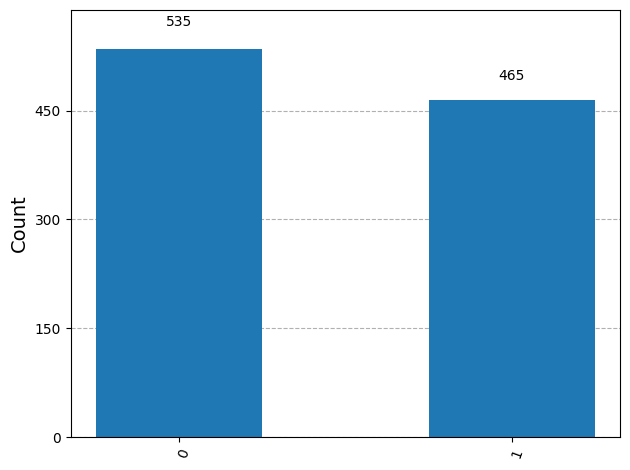
\includegraphics[width=0.55\textwidth]{histograma_psi.png}
    \caption{Resultados de $1000$ mediciones simuladas del estado $|\psi\rangle = \frac{1+2i}{3}|0\rangle - \frac23|1\rangle$. En esta ejecución (distinta de la de la tabla) se obtuvo $535$ veces $0$ y $465$ veces $1$.}
    \label{fig:histograma_psi}
\end{figure}

\begin{tcolorbox}[colback=blue!5!white,colframe=blue!75!black,title=\textbf{Nota Aclaratoria: Cuánto se equivoca la estimación}]
Cada disparo es una variable de Bernoulli que vale $1$ (resultado $0$) con probabilidad $p = 5/9$. La frecuencia observada $\hat p$ es la media de $N$ de estas variables independientes, así que $\mathbb{E}[\hat p] = p$ y
\[ \mathrm{Var}(\hat p) = \frac{p(1-p)}{N}, \qquad \text{es decir, un error típico de } \sqrt{\frac{p(1-p)}{N}} \approx \frac{0.5}{\sqrt N}. \]
Por la \textbf{ley de los grandes números}, $\hat p \to p$ al crecer $N$; y el error decrece como $1/\sqrt N$: para ganar un decimal de precisión hay que multiplicar el número de disparos por $100$. Con $N = 1000$ el error típico es de unos $0.016$, lo que explica que en el histograma no aparezcan exactamente $556$ y $444$.

\textbf{Conexión con el TFG:} cada entrada del kernel cuántico $K(\mathbf{x}, \mathbf{y})$ se estima exactamente así, como la frecuencia de un resultado de medición. Por tanto, la matriz $K$ que recibe la SVM tendrá un error estadístico del orden de $1/\sqrt{N}$, y estudiar su efecto sobre la clasificación es uno de los experimentos previstos.
\end{tcolorbox}

\subsection{Experimento 3: fase global}

\noindent Al medir $|\psi\rangle$ con \texttt{measure()}, Qiskit devuelve el resultado y el estado tras la medición:
\begin{lstlisting}
resultado, estado = psi.measure()
print("Resultado:", resultado)
print("Estado tras medir:", estado.draw("latex_source"))

cero, uno = Statevector.from_label("0"), Statevector.from_label("1")
esperado = cero if resultado == "0" else uno
print("Igual salvo fase global:", estado.equiv(esperado))
print("Igual como vector:      ", np.allclose(estado.data, esperado.data))
\end{lstlisting}

\noindent Según la regla de Born, el estado tras medir debería ser $|0\rangle$ o $|1\rangle$, pero Qiskit devuelve $\frac{1+2i}{\sqrt 5}|0\rangle$ o $-|1\rangle$. No es un error: Qiskit conserva la fase de la amplitud medida y renormaliza. Como $\left|\frac{1+2i}{\sqrt5}\right| = 1$ y $|-1| = 1$, ambos coinciden con $|0\rangle$ y $|1\rangle$ \textbf{salvo una fase global}, y por tanto representan el mismo estado físico. La salida lo confirma: \texttt{equiv} devuelve \texttt{True} (iguales salvo fase global), pero la comparación entrada a entrada devuelve \texttt{False}.
En nuestra ejecución el resultado fue $0$.

\subsection{Experimento 4: interferencia}

\noindent Comprobamos que $|+\rangle$ y $|-\rangle$ no se distinguen midiendo directamente, pero sí aplicando antes $H$:
\begin{lstlisting}
H = Operator.from_label("H")
mas, menos = Statevector.from_label("+"), Statevector.from_label("-")

def probs(estado):
    """Probabilidades de Born, redondeadas a 4 decimales."""
    return {k: round(float(p), 4) for k, p in estado.probabilities_dict().items()}

print("Medida directa |+>:", probs(mas))
print("Medida directa |->:", probs(menos))
print("Tras H         |+>:", probs(mas.evolve(H)))
print("Tras H         |->:", probs(menos.evolve(H)))
\end{lstlisting}

\noindent La salida obtenida es:
\begin{lstlisting}[language={}]
Medida directa |+>: {'0': 0.5, '1': 0.5}
Medida directa |->: {'0': 0.5, '1': 0.5}
Tras H         |+>: {'0': 1.0}
Tras H         |->: {'1': 1.0}
\end{lstlisting}

\noindent Sin redondear, Qiskit devuelve valores como $0.4999999999999999$ o $0.9999999999999996$: son errores de redondeo del orden de $10^{-16}$, debidos a que $1/\sqrt2$ no puede representarse exactamente en coma flotante. Obsérvese también que, tras aplicar $H$, el resultado de probabilidad nula ni siquiera aparece: su amplitud se ha cancelado por completo por interferencia destructiva.

\subsection{Experimento 5: raíz cuadrada de NOT}

\noindent Construimos $R = HSH$ como circuito, lo aplicamos dos veces y comparamos con $X$:
\begin{lstlisting}
R = QuantumCircuit(1)
R.h(0); R.s(0); R.h(0)
print(np.round(Operator.from_circuit(R).data, 4))

R2 = R.compose(R)                       # aplicar R dos veces
X = Operator.from_label("X")
print("R^2 == X:", Operator.from_circuit(R2).equiv(X))
\end{lstlisting}

\noindent La matriz de $R$ es $\frac12\begin{pmatrix} 1+i & 1-i \\ 1-i & 1+i\end{pmatrix}$, como se calculó a mano, y la de $R^2$ coincide con $X$. Hay que tener en cuenta que \texttt{equiv} compara \textbf{salvo fase global} (también daría \texttt{True} para $-X$ o $iX$); en este caso la igualdad es exacta, como se ve a mano: $R^2 = HSHHSH = HS^2H = HZH = X$.

\begin{figure}[htbp]
    \centering
    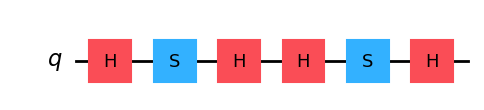
\includegraphics[width=0.6\textwidth]{circuito_R2.png} 
    \caption{Circuito que aplica dos veces $R = HSH$. Las puertas se aplican de izquierda a derecha, mientras que en el producto de matrices el orden es el inverso: el circuito corresponde a $HSH\,HSH$ leído de derecha a izquierda.}
    \label{fig:circuito_R2}
\end{figure}

\subsection{Experimento 6: unitariedad de las puertas}

\noindent Por último, comprobamos numéricamente que $U^\dagger U = \mathbb{I}$ para todas las puertas de la Sección 1.2:
\begin{lstlisting}
for nombre in ["X", "Y", "Z", "H", "S", "T"]:
    U = Operator.from_label(nombre).data
    print(nombre, np.allclose(U.conj().T @ U, np.eye(2)))
\end{lstlisting}
\noindent Todas devuelven \texttt{True}. La función \texttt{np.allclose} compara con una tolerancia pequeña porque la aritmética en coma flotante introduce errores de redondeo (por ejemplo, $1/\sqrt2$ no se representa exactamente).

\providecommand{\pasoguiado}[3]{%
\begin{tcolorbox}[colback=gray!6!white,colframe=gray!55!black,fonttitle=\bfseries,title={#1}]
#2
\tcblower
\small #3
\end{tcolorbox}}

\cleardoublepage
\section{Resumen: un ejemplo guiado}

\noindent Seguimos una única historia: un solo sistema, primero una moneda (caso clásico) y después un qubit (caso cuántico). En cada paso aparece uno de los conceptos del capítulo. En cada caja, la parte superior es el cálculo y la inferior, el concepto.

\subsection{Parte 1: una moneda}

\pasoguiado{Paso 1. ¿En qué estados puede estar?}
{Una moneda puede estar en $0$ (cara) o en $1$ (cruz).}
{\textbf{Estados clásicos:} las configuraciones posibles, que forman un conjunto finito $\Sigma$. Aquí $\Sigma = \{0,1\}$ y el sistema es un \textbf{bit}.}

\pasoguiado{Paso 2. No sabemos cómo ha caído}
{Moneda trucada y tapada: $\Pr(0) = \frac34$, $\Pr(1) = \frac14$.
\[ u = \begin{pmatrix}3/4\\1/4\end{pmatrix} = \tfrac34|0\rangle + \tfrac14|1\rangle, \qquad |0\rangle = \begin{pmatrix}1\\0\end{pmatrix},\ |1\rangle = \begin{pmatrix}0\\1\end{pmatrix}. \]}
{\textbf{Vector de probabilidad:} entradas $\ge 0$ que suman $1$; describe \textbf{lo que sabemos} del sistema. \textbf{Base estándar y notación ket:} $|0\rangle$ y $|1\rangle$ son la base canónica.}

\pasoguiado{Paso 3. Destapamos la moneda}
{Vemos $1$: \quad $\tfrac34|0\rangle + \tfrac14|1\rangle \;\longrightarrow\; |1\rangle$.}
{\textbf{Medición:} se ve un solo estado clásico, elegido según las probabilidades, y el vector pasa a ser $|a\rangle$. La moneda no cambia (ya era $1$); cambia \textbf{nuestra información}.}

\pasoguiado{Paso 4. Le damos la vuelta (NOT)}
{\[ \underbrace{\begin{pmatrix}0&1\\1&0\end{pmatrix}}_{\text{NOT}}\begin{pmatrix}3/4\\1/4\end{pmatrix} = \begin{pmatrix}1/4\\3/4\end{pmatrix}, \qquad \text{NOT} = |1\rangle\langle0| + |0\rangle\langle1|. \]}
{\textbf{Operación determinista:} una función $f:\Sigma\to\Sigma$; su matriz tiene \textbf{un $1$ por columna}, y \textbf{la columna $a$ es lo que sale si entra $a$}. \textbf{Notación de Dirac:} $\langle a|$ (bra) es un vector fila; ket por bra da una matriz.}

\pasoguiado{Paso 5. Una operación que pierde información}
{``Poner a $0$'': \quad $\begin{pmatrix}1&1\\0&0\end{pmatrix}\begin{pmatrix}3/4\\1/4\end{pmatrix} = \begin{pmatrix}1\\0\end{pmatrix}$, \quad con determinante $0$.}
{\textbf{Pérdida de información:} las operaciones constantes no son invertibles; no se puede saber cómo estaba la moneda. En el mundo cuántico, en cambio, \textbf{todas las operaciones unitarias son invertibles} (la medición no lo es).}

\pasoguiado{Paso 6. Una operación con azar}
{``Si es $1$, ponerla a $0$ con probabilidad $\frac12$'':
\[ M = \begin{pmatrix}1&1/2\\0&1/2\end{pmatrix} = \tfrac12\begin{pmatrix}1&0\\0&1\end{pmatrix} + \tfrac12\begin{pmatrix}1&1\\0&0\end{pmatrix}, \qquad M\begin{pmatrix}3/4\\1/4\end{pmatrix} = \begin{pmatrix}7/8\\1/8\end{pmatrix}. \]}
{\textbf{Matriz estocástica:} entradas $\ge0$ y \textbf{cada columna suma $1$}; son exactamente las que transforman vectores de probabilidad en vectores de probabilidad. Toda operación probabilística es una \textbf{mezcla al azar de operaciones deterministas}.}

\pasoguiado{Paso 7. El orden importa}
{Poner a $0$ y después NOT: siempre acaba en $1$. \quad NOT y después poner a $0$: siempre acaba en $0$.}
{\textbf{Composición = producto de matrices}, con la \textbf{primera operación a la derecha}: aplicar $M_1$ y después $M_2$ es $M_2M_1$. El producto de matrices no es conmutativo.}

\subsection{Parte 2: un qubit}

\pasoguiado{Paso 8. Un estado cuántico}
{\[ |\psi\rangle = \tfrac{1+2i}{3}|0\rangle - \tfrac23|1\rangle, \qquad \left|\tfrac{1+2i}{3}\right|^2 + \left|-\tfrac23\right|^2 = \tfrac59 + \tfrac49 = 1. \]}
{\textbf{Vector de estado cuántico:} vector complejo de \textbf{norma $1$} (suma de módulos al cuadrado igual a $1$). \textbf{Qubit:} sistema cuántico con estados clásicos $\{0,1\}$. \textbf{Superposición} = combinación lineal de $|0\rangle$ y $|1\rangle$.}

\pasoguiado{Paso 9. Medimos el qubit}
{$\Pr(0) = \frac59$, \quad $\Pr(1) = \frac49$; \quad tras medir, el estado pasa a ser $|0\rangle$ o $|1\rangle$. \quad $\langle\psi| = \left(\tfrac{1-2i}{3},\ -\tfrac23\right)$.}
{\textbf{Regla de Born:} $\Pr(a) = |\langle a|\psi\rangle|^2$. \textbf{El bra lleva conjugado} ($\langle\psi| = |\psi\rangle^\dagger$) para que $\langle\psi|\psi\rangle = \|\psi\|^2$; sin conjugar, $(1,i)$ tendría ``longitud'' $0$.}

\pasoguiado{Paso 10. Dos estados que parecen iguales}
{$|\pm\rangle = \tfrac{1}{\sqrt2}|0\rangle \pm \tfrac{1}{\sqrt2}|1\rangle$: \quad al medirlos, ambos dan $0$ y $1$ con probabilidad $\frac12$.}
{Midiendo directamente \textbf{no se pueden distinguir}. ¿Son el mismo estado?}

\pasoguiado{Paso 11. La Hadamard los distingue}
{\[ H = \tfrac{1}{\sqrt2}\begin{pmatrix}1&1\\1&-1\end{pmatrix}, \qquad H|+\rangle = \begin{pmatrix}\frac12 + \frac12\\[1mm] \frac12 - \frac12\end{pmatrix} = |0\rangle, \qquad H|-\rangle = |1\rangle. \]}
{Aplicando $H$ y midiendo, $|+\rangle$ da $0$ con certeza y $|-\rangle$ da $1$ con certeza. \textbf{Interferencia:} las amplitudes pueden \textbf{cancelarse} ($\frac12 - \frac12 = 0$); las probabilidades clásicas, al ser no negativas, nunca.}

\pasoguiado{Paso 12. ¿Qué signos importan?}
{$|+\rangle$ y $|-\rangle$ difieren en el signo de \textbf{una} amplitud: son distintos. \quad $-|1\rangle$ y $|1\rangle$ difieren en el signo de \textbf{todo} el vector: son el mismo estado.}
{\textbf{Fase relativa} (afecta a algunas amplitudes): cambia el estado. \textbf{Fase global} (multiplica todo el vector): no cambia nada observable. Por eso el \textbf{kernel cuántico lleva módulo al cuadrado}, $|\langle\phi(\mathbf{x})|\phi(\mathbf{y})\rangle|^2$.}

\pasoguiado{Paso 13. Las operaciones cuánticas conservan la norma}
{\[ H|\psi\rangle = \tfrac{-1+2i}{3\sqrt2}|0\rangle + \tfrac{3+2i}{3\sqrt2}|1\rangle, \qquad \tfrac{5}{18} + \tfrac{13}{18} = 1, \qquad H^2 = \mathbb{I}. \]}
{\textbf{Matriz unitaria:} $U^\dagger U = \mathbb{I}$. Equivale a \textbf{conservar la norma}, es decir, a transformar estados cuánticos en estados cuánticos (análogo de las estocásticas). \textbf{Toda unitaria es invertible}, con $U^{-1} = U^\dagger$. Puertas básicas: $X$, $Y$, $Z$, $H$, $P_\theta$, $S$, $T$.}

\pasoguiado{Paso 14. La raíz cuadrada de NOT}
{Clásicamente: la esquina $(1-p)^2 + qp$ de $M^2$ debería ser $0$, lo que obliga a $M = \begin{pmatrix}0&0\\1&1\end{pmatrix}$, y $M^2 \neq X$. \textbf{Imposible.}
Cuánticamente:
\[ R = HSH = \tfrac12\begin{pmatrix}1+i&1-i\\1-i&1+i\end{pmatrix}, \qquad R^2 = X, \]
pues en la esquina de $R^2$ aparece $(1+i)^2 + (1-i)^2 = 2i - 2i = 0$.}
{Hay operaciones cuánticas sin equivalente clásico. La razón de fondo es siempre la misma: \textbf{los números complejos se pueden cancelar y las probabilidades no}.}

\pasoguiado{Paso 15. ¿Qué operaciones valen en los dos mundos?}
{NOT: estocástica y unitaria. \quad Poner a $0$: solo estocástica (no invertible). \quad $H$: solo unitaria (tiene un $-1$).}
{\textbf{Estocástica y unitaria a la vez} $\iff$ \textbf{matriz de permutación} (solo reordena las entradas).}

\begin{center}
\small\renewcommand{\arraystretch}{1.15}
\begin{tabular}{c|l|l}
\textbf{Paso} & \textbf{Qué hicimos} & \textbf{Concepto} \\ \hline
1 & Cara o cruz & Estados clásicos $\Sigma$ \\
2 & Moneda tapada $\left(\frac34,\frac14\right)$ & Vector de probabilidad, base estándar, ket \\
3 & Destapar & Medición = actualizar lo que sabemos \\
4 & Dar la vuelta & Operación determinista, bra y ket \\
5 & Poner a $0$ & Pérdida de información (no invertible) \\
6 & Operación con azar & Matriz estocástica = mezcla de deterministas \\
7 & Dos operaciones seguidas & Composición = producto; el orden importa \\
8 & $\frac{1+2i}{3}|0\rangle - \frac23|1\rangle$ & Estado cuántico, norma $1$, superposición \\
9 & Medir el qubit & Regla de Born; el bra lleva conjugado \\
10 & $|+\rangle$ y $|-\rangle$ & Misma distribución al medir \\
11 & Aplicar $H$ & Interferencia: se distinguen \\
12 & Signos & Fase global frente a fase relativa \\
13 & $H|\psi\rangle$ & Unitaria = conserva la norma = invertible \\
14 & $R = HSH$ & Raíz de NOT: imposible clásicamente \\
15 & NOT en ambos mundos & Estocástica + unitaria = permutación
\end{tabular}
\end{center}

\noindent \textbf{Conexión con el TFG:} el producto interno del paso 9 (con el bra conjugado) es la base del kernel cuántico; el paso 12 explica por qué el kernel lleva módulo al cuadrado; y la regla de Born con $N$ disparos (Sección 1.3) explica por qué el kernel solo puede \textbf{estimarse}.


\chapter{Sistemas múltiples}


\noindent Hasta ahora hemos estudiado un único sistema. En este capítulo consideramos varios sistemas a la vez, por ejemplo varios bits o varios qubits. La idea que guía todo es sencilla: \textbf{varios sistemas vistos conjuntamente son, a su vez, un único sistema}, al que se aplica todo lo visto en el Capítulo 1. La herramienta matemática nueva que aparece es el \textbf{producto tensorial}, que resulta ser la forma de describir la \textbf{independencia} entre sistemas. Como antes, empezamos por el caso clásico, que servirá de referencia para el cuántico.

\cleardoublepage
\section{Información Clásica}

\subsection{Estados clásicos: el producto cartesiano}

\noindent Sea $\mathsf{X}$ un sistema con conjunto de estados clásicos $\Sigma$ e $\mathsf{Y}$ otro sistema con conjunto de estados clásicos $\Gamma$ (ambos finitos y no vacíos; puede ser $\Sigma = \Gamma$, pero usamos nombres distintos por claridad). Si colocamos los dos sistemas uno junto al otro, $\mathsf{X}$ a la izquierda e $\mathsf{Y}$ a la derecha, podemos verlos como un único sistema compuesto, que denotamos $(\mathsf{X}, \mathsf{Y})$ o $\mathsf{XY}$. Sus estados clásicos forman el \textbf{producto cartesiano}
\[ \Sigma \times \Gamma = \{\, (a, b) \;:\; a \in \Sigma, \; b \in \Gamma \,\}. \]
Que $(\mathsf{X}, \mathsf{Y})$ esté en el estado $(a,b)$ significa exactamente que $\mathsf{X}$ está en $a$ e $\mathsf{Y}$ está en $b$. Por ejemplo, si $\Sigma = \{0,1\}$ y $\Gamma = \{\clubsuit, \diamondsuit, \heartsuit, \spadesuit\}$, el sistema compuesto tiene $8$ estados clásicos: $(0,\clubsuit), (0,\diamondsuit), \dots, (1,\spadesuit)$.

\noindent Para $n$ sistemas $\mathsf{X}_1, \dots, \mathsf{X}_n$ con conjuntos de estados $\Sigma_1, \dots, \Sigma_n$, el conjunto de estados clásicos del sistema compuesto $(\mathsf{X}_1, \dots, \mathsf{X}_n)$ es
\[ \Sigma_1 \times \cdots \times \Sigma_n = \{\, (a_1, \dots, a_n) \;:\; a_1 \in \Sigma_1, \dots, a_n \in \Sigma_n \,\}. \]
Como el producto cartesiano de conjuntos finitos y no vacíos es finito y no vacío, el sistema compuesto es un sistema en el sentido del Capítulo 1, y además
\[ |\Sigma_1 \times \cdots \times \Sigma_n| = |\Sigma_1| \cdots |\Sigma_n|. \]

\noindent Es habitual escribir la $n$-tupla $(a_1, \dots, a_n)$ como una \textbf{cadena} $a_1 \cdots a_n$, sobre todo cuando los estados son símbolos. En este contexto, a los conjuntos de estados clásicos se les llama \textbf{alfabetos}; la definición matemática es la misma: un conjunto finito y no vacío.

\begin{tcolorbox}[colback=blue!5!white,colframe=blue!75!black,title=\textbf{Nota Aclaratoria: La convención de Qiskit (numeración de derecha a izquierda)}]
Podemos nombrar y ordenar los sistemas como queramos. Una convención muy usada, y la que sigue \textbf{Qiskit}, es numerarlos desde $0$ y colocarlos \textbf{de derecha a izquierda}: los sistemas se llaman $\mathsf{X}_0, \dots, \mathsf{X}_{n-1}$, el sistema compuesto es $(\mathsf{X}_{n-1}, \dots, \mathsf{X}_0)$ y sus estados clásicos se escriben
\[ (a_{n-1}, \dots, a_0) \in \Sigma_{n-1} \times \cdots \times \Sigma_0, \qquad \text{o como cadena } a_{n-1} \cdots a_0. \]
Por ejemplo, si $\mathsf{X}_0, \dots, \mathsf{X}_9$ son bits, el sistema compuesto tiene $2^{10} = 1024$ estados clásicos, las cadenas de $\{0,1\}^{10}$:
\[ 0000000000,\; 0000000001,\; 0000000010,\; 0000000011,\; \dots,\; 1111111111. \]
En el estado $0000000110$, los bits $\mathsf{X}_1$ y $\mathsf{X}_2$ valen $1$ y todos los demás valen $0$: el bit $\mathsf{X}_0$ es el \textbf{último} carácter de la cadena, no el primero. Esta convención es fuente frecuente de errores al comparar resultados de Qiskit con fórmulas en papel.
\end{tcolorbox}

\noindent Obsérvese el crecimiento: con $n$ bits hay $2^n$ estados clásicos. Esta cantidad exponencial será la dimensión del espacio de estados de $n$ qubits, el ``espacio de características'' de gran dimensión del que hablan los métodos de kernel cuánticos.

\subsection{Ordenación de los productos cartesianos}

\noindent Para representar estados mediante vectores hay que fijar un orden en el conjunto de estados clásicos (Sección 1.1). Para un producto cartesiano la convención es: partiendo de los órdenes ya fijados en cada conjunto, se ordenan los elementos del producto \textbf{lexicográficamente}, como en un diccionario. Dicho de otro modo, la importancia de cada posición de la tupla (o de cada símbolo de la cadena) \textbf{decrece de izquierda a derecha}. Por ejemplo, $\{1,2,3\} \times \{0,1\}$ se ordena así:
\[ (1,0),\; (1,1),\; (2,0),\; (2,1),\; (3,0),\; (3,1). \]
Con esta convención, $\{0,1\} \times \{0,1\}$ queda ordenado como $00, 01, 10, 11$, y $\{0,\dots,9\} \times \{0,\dots,9\}$ da los números $00$ a $99$ en orden creciente. No es casualidad: nuestro sistema de numeración posicional usa exactamente esta ordenación.

\begin{tcolorbox}[colback=teal!5!white,colframe=teal!75!black,title=\textbf{Nota Teórica: Qué posición ocupa cada estado}]
Si numeramos los estados desde $0$, con $\Sigma = \{0, 1, \dots, m-1\}$ y $\Gamma = \{0, 1, \dots, k-1\}$, el orden lexicográfico coloca el par $(a, b)$ en la posición
\[ \mathrm{pos}(a, b) = a\,k + b \qquad (0 \le \mathrm{pos}(a,b) \le mk - 1). \]
En efecto, antes de los pares que empiezan por $a$ van los $a$ bloques de $k$ pares que empiezan por $0, 1, \dots, a-1$, y dentro de su bloque $(a,b)$ ocupa el lugar $b$. La aplicación $(a,b) \mapsto ak + b$ es una biyección entre $\Sigma \times \Gamma$ y $\{0, \dots, mk-1\}$ (es la división euclídea por $k$: cociente $a$, resto $b$).

Para $n$ bits, aplicando esto repetidamente, la cadena $a_{n-1}\cdots a_1 a_0$ ocupa la posición
\[ \sum_{j=0}^{n-1} a_j\, 2^j, \]
es decir, \textbf{la posición de una cadena de bits es el número que representa en binario}. Por ejemplo, en un vector de $3$ bits, la entrada correspondiente a $101$ es la de índice $5$. Con la convención de Qiskit, el bit $\mathsf{X}_j$ es precisamente el que pesa $2^j$.
\end{tcolorbox}

\subsection{Estados probabilísticos y correlación}

\noindent Un estado probabilístico de varios sistemas, vistos como uno solo, asigna una probabilidad a cada elemento del producto cartesiano. Por ejemplo, para dos bits $\mathsf{X}$ e $\mathsf{Y}$:
\begin{align*}
\Pr\big((\mathsf{X},\mathsf{Y}) = (0,0)\big) &= \tfrac12, &
\Pr\big((\mathsf{X},\mathsf{Y}) = (0,1)\big) &= 0, \\
\Pr\big((\mathsf{X},\mathsf{Y}) = (1,0)\big) &= 0, &
\Pr\big((\mathsf{X},\mathsf{Y}) = (1,1)\big) &= \tfrac12.
\end{align*}
Con la ordenación lexicográfica, este estado se representa por el vector de probabilidad
\begin{equation}\label{eq:correlado}
\begin{pmatrix} 1/2 \\ 0 \\ 0 \\ 1/2 \end{pmatrix}
\begin{array}{l} \leftarrow \text{probabilidad del estado } 00 \\ \leftarrow \text{probabilidad del estado } 01 \\ \leftarrow \text{probabilidad del estado } 10 \\ \leftarrow \text{probabilidad del estado } 11 \end{array}
\qquad = \frac12|00\rangle + \frac12|11\rangle.
\end{equation}
En este estado, cada bit por separado es completamente aleatorio (vale $0$ o $1$ con probabilidad $1/2$), pero \textbf{los dos bits siempre coinciden}. Es un ejemplo de \textbf{correlación} entre sistemas: conocer uno de ellos determina el otro.

\subsection{Independencia de dos sistemas}

\noindent Intuitivamente, dos sistemas son \textbf{independientes} si conocer el estado de uno no aporta ninguna información sobre el otro.

\begin{tcolorbox}[colback=teal!5!white,colframe=teal!75!black,title=\textbf{Definición: Independencia y correlación}]
Dado un estado probabilístico de $(\mathsf{X}, \mathsf{Y})$, los sistemas $\mathsf{X}$ e $\mathsf{Y}$ son \textbf{independientes} si
\begin{equation}\label{eq:indep}
\Pr\big((\mathsf{X}, \mathsf{Y}) = (a, b)\big) = \Pr(\mathsf{X} = a)\,\Pr(\mathsf{Y} = b) \qquad \text{para todos } a \in \Sigma,\ b \in \Gamma.
\end{equation}
Si no son independientes, se dice que están \textbf{correlacionados}: la correlación es, por definición, la falta de independencia.
\end{tcolorbox}

\noindent Aquí $\Pr(\mathsf{X} = a)$ es la probabilidad de que $\mathsf{X}$ esté en $a$, sea cual sea el estado de $\mathsf{Y}$, es decir, la \textbf{probabilidad marginal} $\Pr(\mathsf{X}=a) = \sum_{b \in \Gamma} \Pr\big((\mathsf{X},\mathsf{Y}) = (a,b)\big)$ (se justifica con más detalle al hablar de mediciones parciales). Para expresar la independencia en términos de vectores, escribimos el estado como
\[ |\pi\rangle = \sum_{(a,b) \in \Sigma \times \Gamma} p_{ab}\, |ab\rangle, \qquad p_{ab} = \Pr\big((\mathsf{X},\mathsf{Y}) = (a,b)\big). \]

\begin{tcolorbox}[colback=teal!5!white,colframe=teal!75!black,title=\textbf{Proposición: Independencia en términos de vectores}]
$\mathsf{X}$ e $\mathsf{Y}$ son independientes si y solo si existen vectores de probabilidad
\[ |\phi\rangle = \sum_{a \in \Sigma} q_a |a\rangle \qquad \text{y} \qquad |\psi\rangle = \sum_{b \in \Gamma} r_b |b\rangle \]
tales que $p_{ab} = q_a r_b$ para todos $a \in \Sigma$, $b \in \Gamma$. En ese caso, necesariamente $q_a = \Pr(\mathsf{X} = a)$ y $r_b = \Pr(\mathsf{Y} = b)$.
\end{tcolorbox}

\begin{tcolorbox}[colback=gray!5!white,colframe=gray!75!black,title=\textbf{Demostración}]
($\Rightarrow$) Basta tomar $q_a = \Pr(\mathsf{X}=a)$ y $r_b = \Pr(\mathsf{Y}=b)$: son vectores de probabilidad (las marginales son no negativas y suman $1$) y la condición \eqref{eq:indep} dice exactamente $p_{ab} = q_a r_b$.

($\Leftarrow$) Supongamos $p_{ab} = q_a r_b$ con $q$ y $r$ vectores de probabilidad. Calculamos las marginales:
\[ \Pr(\mathsf{X}=a) = \sum_{b \in \Gamma} p_{ab} = q_a \sum_{b \in \Gamma} r_b = q_a, \qquad \Pr(\mathsf{Y}=b) = \sum_{a \in \Sigma} p_{ab} = r_b \sum_{a \in \Sigma} q_a = r_b. \]
Por tanto $p_{ab} = q_a r_b = \Pr(\mathsf{X}=a)\Pr(\mathsf{Y}=b)$, que es \eqref{eq:indep}. El mismo cálculo prueba la última afirmación. \hfill $\square$
\end{tcolorbox}

\begin{tcolorbox}[colback=cyan!5!white,colframe=cyan!75!black,title=\textbf{Ejemplo: Un estado independiente y uno correlacionado}]
\textbf{Independiente.} El estado de dos bits
\[ \tfrac16|00\rangle + \tfrac{1}{12}|01\rangle + \tfrac12|10\rangle + \tfrac14|11\rangle \]
es independiente, con $|\phi\rangle = \frac14|0\rangle + \frac34|1\rangle$ y $|\psi\rangle = \frac23|0\rangle + \frac13|1\rangle$. En efecto: $\frac14\cdot\frac23 = \frac16$, $\frac14\cdot\frac13 = \frac1{12}$, $\frac34\cdot\frac23 = \frac12$ y $\frac34\cdot\frac13 = \frac14$.

\textbf{Correlacionado.} El estado \eqref{eq:correlado}, $\frac12|00\rangle + \frac12|11\rangle$, no es independiente. Si existieran $q_0, q_1, r_0, r_1$ con $p_{ab} = q_a r_b$, tendríamos
\[ q_0 r_1 = p_{01} = 0, \qquad q_0 r_0 = p_{00} = \tfrac12, \qquad q_1 r_1 = p_{11} = \tfrac12. \]
De la primera igualdad, $q_0 = 0$ o $r_1 = 0$; en el primer caso $q_0 r_0 = 0$, y en el segundo $q_1 r_1 = 0$. Ambas cosas contradicen las otras dos igualdades.
\end{tcolorbox}

\noindent Hay una forma más sistemática de detectar la independencia, que conviene conocer porque reaparecerá en el caso cuántico al estudiar el entrelazamiento. Organicemos las probabilidades $p_{ab}$ en una \textbf{matriz} $P = (p_{ab})$ con filas indexadas por $\Sigma$ y columnas por $\Gamma$.

\begin{tcolorbox}[colback=teal!5!white,colframe=teal!75!black,title=\textbf{Proposición: Criterio del rango}]
$\mathsf{X}$ e $\mathsf{Y}$ son independientes si y solo si la matriz $P = (p_{ab})$ tiene \textbf{rango 1}. En particular, para dos bits,
\[ \mathsf{X} \text{ e } \mathsf{Y} \text{ independientes} \iff p_{00}\,p_{11} = p_{01}\,p_{10}. \]
\end{tcolorbox}

\begin{tcolorbox}[colback=gray!5!white,colframe=gray!75!black,title=\textbf{Demostración}]
La condición $p_{ab} = q_a r_b$ para todos $a, b$ se escribe matricialmente como $P = q\, r^T$ (columna por fila). Si se cumple, $P$ tiene rango $1$ (es no nula, porque sus entradas suman $1$, y todas sus columnas son múltiplos de $q$).

Recíprocamente, si $P$ tiene rango $1$, todas sus filas son múltiplos de una misma fila no nula, así que $P = u\, v^T$ para ciertos vectores $u, v$. Como $P$ tiene entradas no negativas, podemos elegir $u$ y $v$ con entradas no negativas (tomando $v$ como una fila no nula de $P$, que tiene entradas no negativas, y $u_a \ge 0$ como el factor por el que se multiplica). Sean $s = \sum_a u_a > 0$ y $t = \sum_b v_b > 0$. Como $\sum_{a,b} p_{ab} = st = 1$, los vectores $q = u/s$ y $r = v/t$ son de probabilidad y $P = q\,r^T$.

Para dos bits, una matriz $2 \times 2$ no nula tiene rango $1$ si y solo si su determinante es nulo: $p_{00}p_{11} - p_{01}p_{10} = 0$. \hfill $\square$

\textit{Comprobación:} en el ejemplo independiente, $\frac16 \cdot \frac14 = \frac1{24} = \frac1{12}\cdot\frac12$. En el correlacionado, $\frac12 \cdot \frac12 \neq 0 \cdot 0$.
\end{tcolorbox}

\subsection{Producto tensorial de vectores}

\noindent La condición de independencia se expresa de forma compacta mediante el \textbf{producto tensorial}. Aunque es una noción muy general, aquí basta una definición concreta.

\begin{tcolorbox}[colback=teal!5!white,colframe=teal!75!black,title=\textbf{Definición: Producto tensorial de vectores}]
Dados $|\phi\rangle = \sum_{a \in \Sigma} \alpha_a |a\rangle \in \mathbb{C}^\Sigma$ y $|\psi\rangle = \sum_{b \in \Gamma} \beta_b |b\rangle \in \mathbb{C}^\Gamma$, su \textbf{producto tensorial} es el vector de $\mathbb{C}^{\Sigma \times \Gamma}$
\[ |\phi\rangle \otimes |\psi\rangle = \sum_{(a,b) \in \Sigma \times \Gamma} \alpha_a \beta_b\, |ab\rangle. \]
Equivalentemente, $|\pi\rangle = |\phi\rangle \otimes |\psi\rangle$ es el vector cuyas entradas son
\[ \langle ab|\pi\rangle = \langle a|\phi\rangle\,\langle b|\psi\rangle \qquad \text{para todos } a \in \Sigma,\ b \in \Gamma. \]
Notaciones alternativas: $|\phi\rangle|\psi\rangle$ (se omite $\otimes$, por ser el producto ``natural'' entre kets) y, menos habitual, $|\phi \otimes \psi\rangle$.
\end{tcolorbox}

\noindent Con la ordenación lexicográfica, el producto tensorial de dos vectores columna es:
\[
\begin{pmatrix} \alpha_1 \\ \vdots \\ \alpha_m \end{pmatrix} \otimes \begin{pmatrix} \beta_1 \\ \vdots \\ \beta_k \end{pmatrix}
= \begin{pmatrix} \alpha_1 \beta_1 \\ \vdots \\ \alpha_1 \beta_k \\ \alpha_2\beta_1 \\ \vdots \\ \alpha_m \beta_k \end{pmatrix}
= \begin{pmatrix} \alpha_1 \begin{pmatrix} \beta_1 \\ \vdots \\ \beta_k \end{pmatrix} \\ \vdots \\ \alpha_m \begin{pmatrix} \beta_1 \\ \vdots \\ \beta_k \end{pmatrix} \end{pmatrix}.
\]
Es decir: \textbf{se copia el segundo vector una vez por cada entrada del primero, multiplicado por esa entrada}. El resultado tiene $mk$ entradas, y la entrada de posición $(i-1)k + j$ (contando desde $1$) es $\alpha_i \beta_j$, de acuerdo con la fórmula de posiciones anterior. Por ejemplo,
\[ \begin{pmatrix} 1/4 \\ 3/4 \end{pmatrix} \otimes \begin{pmatrix} 2/3 \\ 1/3 \end{pmatrix} = \begin{pmatrix} 1/6 \\ 1/12 \\ 1/2 \\ 1/4 \end{pmatrix}, \]
que es el estado independiente del ejemplo anterior. En general:
\begin{center}
\fbox{\parbox{0.85\textwidth}{\centering Un estado probabilístico $|\pi\rangle$ de $(\mathsf{X},\mathsf{Y})$ es independiente si y solo si $|\pi\rangle = |\phi\rangle \otimes |\psi\rangle$ para ciertos vectores de probabilidad $|\phi\rangle$ de $\mathsf{X}$ y $|\psi\rangle$ de $\mathsf{Y}$. Se dice entonces que $|\pi\rangle$ es un \textbf{estado producto}.}}
\end{center}

\noindent Un caso particular importante es el de los vectores de la base estándar:
\[ |a\rangle \otimes |b\rangle = |ab\rangle, \]
que también se escribe $|a, b\rangle$ (se omiten los paréntesis del par ordenado cuando no añaden claridad). Así, por ejemplo, $|0\rangle \otimes |1\rangle = |01\rangle = (0, 1, 0, 0)^T$.

\begin{tcolorbox}[colback=teal!5!white,colframe=teal!75!black,title=\textbf{Proposición: Propiedades del producto tensorial de vectores}]
Para vectores $|\phi\rangle, |\phi_1\rangle, |\phi_2\rangle \in \mathbb{C}^\Sigma$, $|\psi\rangle, |\psi_1\rangle, |\psi_2\rangle \in \mathbb{C}^\Gamma$ y escalares $\alpha \in \mathbb{C}$:
\begin{enumerate}
    \item \textbf{Bilinealidad} (lineal en cada argumento, fijado el otro):
    \begin{align*}
    (|\phi_1\rangle + |\phi_2\rangle) \otimes |\psi\rangle &= |\phi_1\rangle \otimes |\psi\rangle + |\phi_2\rangle \otimes |\psi\rangle, &
    (\alpha|\phi\rangle) \otimes |\psi\rangle &= \alpha\,(|\phi\rangle \otimes |\psi\rangle), \\
    |\phi\rangle \otimes (|\psi_1\rangle + |\psi_2\rangle) &= |\phi\rangle \otimes |\psi_1\rangle + |\phi\rangle \otimes |\psi_2\rangle, &
    |\phi\rangle \otimes (\alpha|\psi\rangle) &= \alpha\,(|\phi\rangle \otimes |\psi\rangle).
    \end{align*}
    En particular, los escalares ``flotan libremente'': $(\alpha|\phi\rangle)\otimes|\psi\rangle = |\phi\rangle \otimes (\alpha|\psi\rangle) = \alpha\,|\phi\rangle|\psi\rangle$, así que escribir $\alpha|\phi\rangle|\psi\rangle$ no es ambiguo.
    \item \textbf{Producto interno multiplicativo}:
    \[ \big\langle \phi_1 \otimes \psi_1 \,\big|\, \phi_2 \otimes \psi_2 \big\rangle = \langle \phi_1|\phi_2\rangle\,\langle\psi_1|\psi_2\rangle. \]
    En particular, $\big\| |\phi\rangle \otimes |\psi\rangle \big\| = \big\||\phi\rangle\big\|\,\big\||\psi\rangle\big\|$.
    \item \textbf{Producto de vectores de probabilidad}: si $|\phi\rangle$ y $|\psi\rangle$ son vectores de probabilidad, $|\phi\rangle\otimes|\psi\rangle$ también lo es.
    \item \textbf{No conmutatividad}: en general $|\phi\rangle \otimes |\psi\rangle \neq |\psi\rangle \otimes |\phi\rangle$ (incluso cuando $\Sigma = \Gamma$). Por ejemplo, $|0\rangle\otimes|1\rangle = |01\rangle \neq |10\rangle = |1\rangle\otimes|0\rangle$.
\end{enumerate}
\end{tcolorbox}

\begin{tcolorbox}[colback=gray!5!white,colframe=gray!75!black,title=\textbf{Demostración}]
Todo se comprueba entrada a entrada usando $\langle ab|\phi\otimes\psi\rangle = \langle a|\phi\rangle\langle b|\psi\rangle$.

1. La entrada $(a,b)$ de $(|\phi_1\rangle + |\phi_2\rangle)\otimes|\psi\rangle$ es $\big(\langle a|\phi_1\rangle + \langle a|\phi_2\rangle\big)\langle b|\psi\rangle$, que por la propiedad distributiva de los números es la suma de las entradas $(a,b)$ de los dos productos de la derecha. Las demás igualdades son análogas.

2. Usando la definición de producto interno complejo y separando la suma doble,
\begin{align*}
\big\langle \phi_1 \otimes \psi_1 \,\big|\, \phi_2 \otimes \psi_2 \big\rangle
&= \sum_{a,b} \overline{\langle a|\phi_1\rangle\langle b|\psi_1\rangle}\;\langle a|\phi_2\rangle\langle b|\psi_2\rangle \\
&= \Big(\sum_a \overline{\langle a|\phi_1\rangle}\langle a|\phi_2\rangle\Big)\Big(\sum_b \overline{\langle b|\psi_1\rangle}\langle b|\psi_2\rangle\Big),
\end{align*}
que es $\langle\phi_1|\phi_2\rangle\langle\psi_1|\psi_2\rangle$. Tomando $\phi_1 = \phi_2$ y $\psi_1 = \psi_2$ y extrayendo raíces se obtiene la igualdad de normas.

3. Las entradas $q_a r_b$ son productos de números no negativos, y $\sum_{a,b} q_a r_b = \big(\sum_a q_a\big)\big(\sum_b r_b\big) = 1 \cdot 1 = 1$. \hfill $\square$
\end{tcolorbox}

\begin{tcolorbox}[colback=blue!5!white,colframe=blue!75!black,title=\textbf{Nota Aclaratoria: No todo vector es un producto tensorial}]
El espacio $\mathbb{C}^{\Sigma\times\Gamma}$ tiene dimensión $|\Sigma|\,|\Gamma|$, pero un producto $|\phi\rangle\otimes|\psi\rangle$ se describe con solo $|\Sigma| + |\Gamma|$ números. Para $n$ bits la diferencia es enorme: un vector general tiene $2^n$ entradas, mientras que un producto de $n$ vectores de un bit se describe con $2n$ números. Por eso la mayoría de los vectores del sistema compuesto \textbf{no} son productos: en el caso probabilístico, son estados correlacionados; en el caso cuántico, veremos que corresponden al \textbf{entrelazamiento}.

\textbf{Conexión con el TFG:} la propiedad 2 tiene una consecuencia directa para los kernels cuánticos. Si un mapa de características cuántico produce siempre estados producto, $|\phi(\mathbf{x})\rangle = |\phi_1(x_1)\rangle \otimes\cdots\otimes|\phi_n(x_n)\rangle$, entonces el kernel se factoriza,
\[ K(\mathbf{x},\mathbf{y}) = |\langle\phi(\mathbf{x})|\phi(\mathbf{y})\rangle|^2 = \prod_{j=1}^n |\langle\phi_j(x_j)|\phi_j(y_j)\rangle|^2, \]
y puede calcularse eficientemente en un ordenador clásico. Para aspirar a una ventaja cuántica el mapa debe generar estados \textbf{no} producto, como observan Havlíček et al.\ \cite{havlicek2019supervised}.
\end{tcolorbox}

\subsection{Tres o más sistemas}

\noindent Todo lo anterior se generaliza de forma natural. Si $\mathsf{X}_0, \dots, \mathsf{X}_{n-1}$ tienen conjuntos de estados $\Sigma_0, \dots, \Sigma_{n-1}$, el producto tensorial $|\psi\rangle = |\phi_{n-1}\rangle\otimes\cdots\otimes|\phi_0\rangle$ se define por
\[ \langle a_{n-1}\cdots a_0|\psi\rangle = \langle a_{n-1}|\phi_{n-1}\rangle\cdots\langle a_0|\phi_0\rangle \qquad \text{para todos } a_0\in\Sigma_0,\dots,a_{n-1}\in\Sigma_{n-1}, \]
o, de forma equivalente, recursivamente:
\[ |\phi_{n-1}\rangle\otimes\cdots\otimes|\phi_0\rangle = |\phi_{n-1}\rangle \otimes \big(|\phi_{n-2}\rangle\otimes\cdots\otimes|\phi_0\rangle\big). \]
(La equivalencia se debe a que el producto tensorial es \textbf{asociativo}: $(|\phi\rangle\otimes|\psi\rangle)\otimes|\chi\rangle = |\phi\rangle\otimes(|\psi\rangle\otimes|\chi\rangle)$, pues ambos lados tienen entrada $(a,b,c)$ igual a $\langle a|\phi\rangle\langle b|\psi\rangle\langle c|\chi\rangle$. Por eso se omiten los paréntesis.) El producto de tres o más vectores es \textbf{multilineal}: lineal en cada argumento, fijados los demás. Para vectores de la base estándar,
\[ |a_{n-1}\rangle\otimes\cdots\otimes|a_0\rangle = |a_{n-1}\cdots a_0\rangle. \]
Un estado probabilístico de $(\mathsf{X}_{n-1},\dots,\mathsf{X}_0)$ es un \textbf{estado producto} si es de la forma $|\phi_{n-1}\rangle\otimes\cdots\otimes|\phi_0\rangle$ con cada $|\phi_j\rangle$ vector de probabilidad; se dice entonces que los sistemas son \textbf{mutuamente independientes}. (Existen otras nociones de independencia para tres o más sistemas, como la independencia dos a dos, que no necesitaremos.)

\subsection{Mediciones de estados probabilísticos}

\noindent Si se miden \textbf{todos} los sistemas, no hay nada nuevo: el sistema compuesto es un sistema más. Por ejemplo, si dos bits están en el estado $\frac12|00\rangle + \frac12|11\rangle$, al medir ambos se obtiene $00$ con probabilidad $\frac12$ y $11$ con probabilidad $\frac12$, y el estado se actualiza a $|00\rangle$ o $|11\rangle$ respectivamente.

\noindent Lo interesante es medir \textbf{solo algunos} de los sistemas. Basta estudiar el caso de dos sistemas $(\mathsf{X},\mathsf{Y})$ en el que se mide solo $\mathsf{X}$ (el caso general se reduce a este agrupando los sistemas medidos en uno y los no medidos en otro, y el caso en que se mide solo $\mathsf{Y}$ es simétrico).

\noindent \textbf{1. Probabilidad de cada resultado.} La probabilidad de observar $a \in \Sigma$ al medir solo $\mathsf{X}$ debe coincidir con la que obtendríamos si midiésemos también $\mathsf{Y}$ y después ignorásemos su resultado:
\[ \Pr(\mathsf{X} = a) = \sum_{b\in\Gamma} \Pr\big((\mathsf{X},\mathsf{Y}) = (a,b)\big). \]
Esta es la \textbf{probabilidad marginal} (o estado \textbf{reducido}) de $\mathsf{X}$. Si no fuera así, el mero hecho de medir $\mathsf{Y}$, aunque no conozcamos su resultado, alteraría las probabilidades de $\mathsf{X}$; si $\mathsf{Y}$ estuviera muy lejos (en otra galaxia, por ejemplo), esto permitiría enviar información más rápido que la luz. Desde el punto de vista de las probabilidades como grado de creencia: que otra persona mire $\mathsf{Y}$ no cambia el estado de $\mathsf{X}$, y si no sabemos qué ha visto, nuestra creencia sobre $\mathsf{X}$ no debe cambiar.

\noindent \textbf{2. Estado de $\mathsf{Y}$ tras la medición.} Tras obtener $a$, puede seguir habiendo incertidumbre sobre $\mathsf{Y}$, así que no actualizamos a un $|ab\rangle$ concreto, sino que usamos la \textbf{probabilidad condicionada}:
\[ \Pr(\mathsf{Y} = b \mid \mathsf{X} = a) = \frac{\Pr\big((\mathsf{X},\mathsf{Y}) = (a,b)\big)}{\Pr(\mathsf{X}=a)}. \]
Solo tiene sentido si $\Pr(\mathsf{X}=a) > 0$, pero eso no es un problema: un resultado de probabilidad nula no se obtiene nunca.

\begin{tcolorbox}[colback=teal!5!white,colframe=teal!75!black,title=\textbf{Regla de la medición parcial (caso probabilístico)}]
Sea $|\pi\rangle = \sum_{(a,b)\in\Sigma\times\Gamma} p_{ab}|ab\rangle$ el estado de $(\mathsf{X},\mathsf{Y})$. Si se mide solo $\mathsf{X}$:
\begin{itemize}
    \item Se obtiene $a \in \Sigma$ con probabilidad $\displaystyle\Pr(\mathsf{X}=a) = \sum_{c\in\Gamma} p_{ac}$. Así, el estado reducido de $\mathsf{X}$ es $\displaystyle\sum_{a\in\Sigma}\Big(\sum_{c\in\Gamma} p_{ac}\Big)|a\rangle$.
    \item Condicionado al resultado $a$, el estado de $\mathsf{Y}$ pasa a ser
    \[ |\psi_a\rangle = \frac{\sum_{b\in\Gamma} p_{ab}|b\rangle}{\sum_{c\in\Gamma} p_{ac}}, \]
    y el del sistema compuesto, $|a\rangle\otimes|\psi_a\rangle$.
\end{itemize}
Si se mide solo $\mathsf{Y}$, simétricamente: se obtiene $b\in\Gamma$ con probabilidad $\sum_{c\in\Sigma}p_{cb}$, y el estado de $\mathsf{X}$ pasa a ser $\big(\sum_{a\in\Sigma}p_{ab}|a\rangle\big)\big/\sum_{c\in\Sigma}p_{cb}$.
\end{tcolorbox}

\noindent El vector $|\psi_a\rangle$ se obtiene \textbf{normalizando} $\sum_b p_{ab}|b\rangle$, es decir, dividiéndolo por la suma de sus entradas para que sea un vector de probabilidad. Esa normalización es precisamente el condicionamiento al resultado $a$. En la práctica, el procedimiento es:
\begin{enumerate}
    \item Agrupar el vector según el estado del sistema medido, usando la linealidad del producto tensorial en el segundo argumento: $|\pi\rangle = \sum_a |a\rangle \otimes \big(\sum_b p_{ab}|b\rangle\big)$. Esto siempre es posible.
    \item La probabilidad de $a$ es la suma de las entradas del vector entre paréntesis.
    \item El nuevo estado de $\mathsf{Y}$ es ese vector normalizado.
\end{enumerate}

\begin{tcolorbox}[colback=cyan!5!white,colframe=cyan!75!black,title=\textbf{Ejemplo: Medición parcial}]
Sean $\Sigma = \{0,1\}$, $\Gamma = \{1,2,3\}$ y
\[ |\pi\rangle = \tfrac12|0,1\rangle + \tfrac1{12}|0,3\rangle + \tfrac1{12}|1,1\rangle + \tfrac16|1,2\rangle + \tfrac16|1,3\rangle. \]
\textbf{Medimos $\mathsf{X}$.} Agrupando por el estado de $\mathsf{X}$:
\[ |\pi\rangle = |0\rangle\otimes\Big(\tfrac12|1\rangle + \tfrac1{12}|3\rangle\Big) + |1\rangle\otimes\Big(\tfrac1{12}|1\rangle + \tfrac16|2\rangle + \tfrac16|3\rangle\Big). \]
Las probabilidades son $\Pr(\mathsf{X}=0) = \frac12 + \frac1{12} = \frac7{12}$ y $\Pr(\mathsf{X}=1) = \frac1{12}+\frac16+\frac16 = \frac5{12}$, que suman $1$, como debe ser. Normalizando:
\[ \mathsf{X}=0:\quad \frac{\frac12|1\rangle + \frac1{12}|3\rangle}{7/12} = \tfrac67|1\rangle + \tfrac17|3\rangle, \]
\[ \mathsf{X}=1:\quad \frac{\frac1{12}|1\rangle + \frac16|2\rangle + \frac16|3\rangle}{5/12} = \tfrac15|1\rangle + \tfrac25|2\rangle + \tfrac25|3\rangle. \]

\textbf{Medimos $\mathsf{Y}$ en su lugar.} Agrupando ahora por el estado de $\mathsf{Y}$:
\[ |\pi\rangle = \Big(\tfrac12|0\rangle + \tfrac1{12}|1\rangle\Big)\otimes|1\rangle + \tfrac16|1\rangle\otimes|2\rangle + \Big(\tfrac1{12}|0\rangle + \tfrac16|1\rangle\Big)\otimes|3\rangle, \]
de donde $\Pr(\mathsf{Y}=1) = \frac7{12}$, $\Pr(\mathsf{Y}=2) = \frac16$, $\Pr(\mathsf{Y}=3) = \frac14$, y el estado de $\mathsf{X}$ pasa a ser, respectivamente, $\frac67|0\rangle + \frac17|1\rangle$, \; $|1\rangle$, \; y $\frac13|0\rangle + \frac23|1\rangle$.
\end{tcolorbox}

\subsection{Operaciones sobre estados probabilísticos}

\noindent De nuevo, viendo varios sistemas como uno solo, una operación probabilística sobre $(\mathsf{X},\mathsf{Y})$ es una \textbf{matriz estocástica con filas y columnas indexadas por $\Sigma\times\Gamma$}. Veamos algunos ejemplos con dos bits.

\noindent \textbf{NOT controlado (CNOT).} ``Si $\mathsf{X}=1$, aplicar NOT a $\mathsf{Y}$; si no, no hacer nada.'' Es una operación determinista; $\mathsf{X}$ es el bit de \textbf{control} e $\mathsf{Y}$ el bit \textbf{objetivo}:
\[
|00\rangle\mapsto|00\rangle,\quad |01\rangle\mapsto|01\rangle,\quad |10\rangle\mapsto|11\rangle,\quad |11\rangle\mapsto|10\rangle,
\qquad
\begin{pmatrix} 1&0&0&0\\0&1&0&0\\0&0&0&1\\0&0&1&0 \end{pmatrix}.
\]
Si se intercambian los papeles ($\mathsf{Y}$ control, $\mathsf{X}$ objetivo), la operación es $|00\rangle\mapsto|00\rangle$, $|01\rangle\mapsto|11\rangle$, $|10\rangle\mapsto|10\rangle$, $|11\rangle\mapsto|01\rangle$, con matriz
\[ \begin{pmatrix} 1&0&0&0\\0&0&0&1\\0&0&1&0\\0&1&0&0 \end{pmatrix}. \]
(Recuérdese que la columna correspondiente a $|ab\rangle$ es la imagen de $|ab\rangle$.) Ambas son matrices de permutación, así que serán también operaciones cuánticas válidas.

\noindent \textbf{Una operación probabilística.} ``Con probabilidad $\frac12$, hacer $\mathsf{Y}$ igual a $\mathsf{X}$; con probabilidad $\frac12$, hacer $\mathsf{X}$ igual a $\mathsf{Y}$.'' Es la mezcla de dos operaciones deterministas:
\[
\begin{pmatrix} 1&\frac12&\frac12&0\\0&0&0&0\\0&0&0&0\\0&\frac12&\frac12&1 \end{pmatrix}
= \frac12\begin{pmatrix} 1&1&0&0\\0&0&0&0\\0&0&0&0\\0&0&1&1 \end{pmatrix}
+ \frac12\begin{pmatrix} 1&0&1&0\\0&0&0&0\\0&0&0&0\\0&1&0&1 \end{pmatrix},
\]
con acción $|00\rangle\mapsto|00\rangle$, $|01\rangle\mapsto\frac12|00\rangle+\frac12|11\rangle$, $|10\rangle\mapsto\frac12|00\rangle+\frac12|11\rangle$, $|11\rangle\mapsto|11\rangle$. Obsérvese que \textbf{crea correlación}: partiendo del estado independiente $|01\rangle$ se llega al estado correlacionado $\frac12|00\rangle+\frac12|11\rangle$.

\noindent \textbf{Incremento módulo 8.} Con tres bits que codifican en binario un número de $0$ a $7$, la operación ``sumar $1$ módulo $8$'' se escribe
\[ \sum_{k=0}^{7} |(k+1) \bmod 8\rangle\langle k| = |001\rangle\langle000| + |010\rangle\langle001| + \cdots + |111\rangle\langle110| + |000\rangle\langle111|, \]
entendiendo que el número $k$ dentro de un ket denota su codificación binaria de tres bits. Como matriz $8\times 8$, tiene unos justo debajo de la diagonal y un $1$ en la esquina superior derecha: es la permutación cíclica de las posiciones (generaliza la suma módulo $3$ de la Sección 1.2).

\subsection{Operaciones independientes y producto tensorial de matrices}

\noindent Supongamos ahora que realizamos una operación $M$ sobre $\mathsf{X}$ y, de forma completamente independiente, otra operación $N$ sobre $\mathsf{Y}$. ¿Qué matriz describe la acción conjunta sobre $(\mathsf{X},\mathsf{Y})$? La respuesta es el producto tensorial de matrices.

\begin{tcolorbox}[colback=teal!5!white,colframe=teal!75!black,title=\textbf{Definición: Producto tensorial de matrices}]
Dadas $M = \sum_{a,b\in\Sigma}\alpha_{ab}|a\rangle\langle b|$ y $N = \sum_{c,d\in\Gamma}\beta_{cd}|c\rangle\langle d|$, su producto tensorial es
\[ M\otimes N = \sum_{a,b\in\Sigma}\;\sum_{c,d\in\Gamma} \alpha_{ab}\beta_{cd}\;|ac\rangle\langle bd|, \]
es decir, la matriz con entradas
\[ \langle ac|M\otimes N|bd\rangle = \langle a|M|b\rangle\,\langle c|N|d\rangle \qquad \text{para todos } a,b\in\Sigma,\ c,d\in\Gamma. \]
Equivalentemente, $M\otimes N$ es la \textbf{única} matriz que cumple
\[ (M\otimes N)\big(|\phi\rangle\otimes|\psi\rangle\big) = \big(M|\phi\rangle\big)\otimes\big(N|\psi\rangle\big) \qquad \text{para todos } |\phi\rangle, |\psi\rangle. \]
\end{tcolorbox}

\noindent Con la ordenación lexicográfica, el producto tensorial de matrices (también llamado \textbf{producto de Kronecker}) tiene una forma por bloques muy cómoda de recordar: \textbf{cada entrada de $M$ se sustituye por esa entrada multiplicada por la matriz $N$ completa},
\[
M\otimes N = \begin{pmatrix} \alpha_{11} & \cdots & \alpha_{1m} \\ \vdots & \ddots & \vdots \\ \alpha_{m1} & \cdots & \alpha_{mm}\end{pmatrix} \otimes N
= \begin{pmatrix} \alpha_{11}N & \cdots & \alpha_{1m}N \\ \vdots & \ddots & \vdots \\ \alpha_{m1}N & \cdots & \alpha_{mm}N\end{pmatrix}.
\]
Si $M$ es $m\times m$ y $N$ es $k\times k$, $M\otimes N$ es $mk\times mk$. (La expresión con índices y la de bloques son la misma: el bloque $(a,b)$ de $M\otimes N$ tiene entradas $\alpha_{ab}\beta_{cd}$.)

\begin{tcolorbox}[colback=gray!5!white,colframe=gray!75!black,title=\textbf{Demostración de la caracterización}]
\textit{La matriz definida cumple la propiedad.} Sean $|\phi\rangle = \sum_b \phi_b|b\rangle$ y $|\psi\rangle = \sum_d \psi_d|d\rangle$. La entrada $(a,c)$ de $(M\otimes N)(|\phi\rangle\otimes|\psi\rangle)$ es
\begin{align*} \sum_{b,d}\langle ac|M\otimes N|bd\rangle\,\phi_b\psi_d &= \sum_{b,d}\alpha_{ab}\beta_{cd}\phi_b\psi_d \\ &= \Big(\sum_b\alpha_{ab}\phi_b\Big)\Big(\sum_d\beta_{cd}\psi_d\Big) = \langle a|M\phi\rangle\,\langle c|N\psi\rangle, \end{align*}
que es la entrada $(a,c)$ de $(M|\phi\rangle)\otimes(N|\psi\rangle)$.

\textit{Unicidad.} Los vectores $|b\rangle\otimes|d\rangle = |bd\rangle$ forman la base estándar de $\mathbb{C}^{\Sigma\times\Gamma}$, y una matriz queda determinada por sus imágenes de una base. Si otra matriz $L$ cumple la propiedad, entonces $L|bd\rangle = M|b\rangle\otimes N|d\rangle = (M\otimes N)|bd\rangle$ para todos $b,d$, luego $L = M\otimes N$. \hfill $\square$
\end{tcolorbox}

\noindent Para tres o más matrices, $M_{n-1}\otimes\cdots\otimes M_0$ se define por
\[ \langle a_{n-1}\cdots a_0|M_{n-1}\otimes\cdots\otimes M_0|b_{n-1}\cdots b_0\rangle = \langle a_{n-1}|M_{n-1}|b_{n-1}\rangle\cdots\langle a_0|M_0|b_0\rangle, \]
o recursivamente, igual que con los vectores.

\begin{tcolorbox}[colback=teal!5!white,colframe=teal!75!black,title=\textbf{Proposición: Propiedades del producto tensorial de matrices}]
\begin{enumerate}
    \item \textbf{Multiplicatividad} (propiedad del producto mixto): siempre que los productos $M_jN_j$ tengan sentido,
    \[ (M_{n-1}\otimes\cdots\otimes M_0)(N_{n-1}\otimes\cdots\otimes N_0) = (M_{n-1}N_{n-1})\otimes\cdots\otimes(M_0N_0). \]
    \item $\mathbb{I}_\Sigma\otimes\mathbb{I}_\Gamma = \mathbb{I}_{\Sigma\times\Gamma}$.
    \item Si $M$ y $N$ son \textbf{estocásticas}, $M\otimes N$ también lo es.
\end{enumerate}
\end{tcolorbox}

\begin{tcolorbox}[colback=gray!5!white,colframe=gray!75!black,title=\textbf{Demostración}]
1. Basta el caso de dos factores (el general sigue por inducción usando la definición recursiva). Por la caracterización anterior, aplicada dos veces, para todo producto $|\phi\rangle\otimes|\psi\rangle$:
\[ (M_1\otimes M_0)(N_1\otimes N_0)\big(|\phi\rangle\otimes|\psi\rangle\big) = (M_1\otimes M_0)\big(N_1|\phi\rangle\otimes N_0|\psi\rangle\big) = M_1N_1|\phi\rangle\otimes M_0N_0|\psi\rangle. \]
Por tanto, la matriz de la izquierda cumple la propiedad que caracteriza a $(M_1N_1)\otimes(M_0N_0)$, y por la unicidad son iguales.

2. La entrada $(ac, bd)$ de $\mathbb{I}\otimes\mathbb{I}$ es $\langle a|b\rangle\langle c|d\rangle$, que vale $1$ si $(a,c) = (b,d)$ y $0$ en otro caso.

3. Las entradas $\alpha_{ab}\beta_{cd}$ son no negativas. La suma de la columna $bd$ es $\sum_{a,c}\alpha_{ab}\beta_{cd} = \big(\sum_a\alpha_{ab}\big)\big(\sum_c\beta_{cd}\big) = 1\cdot1 = 1$. \hfill $\square$
\end{tcolorbox}

\noindent Con esto podemos responder a la pregunta: \textbf{si $M$ actúa sobre $\mathsf{X}$ y $N$ sobre $\mathsf{Y}$ de forma independiente, la operación conjunta sobre $(\mathsf{X},\mathsf{Y})$ es $M\otimes N$}. Así, tanto para estados como para operaciones, \textbf{el producto tensorial representa la independencia}: sistemas independientes en los estados $|\phi\rangle$ y $|\psi\rangle$ están conjuntamente en el estado $|\phi\rangle\otimes|\psi\rangle$, y operaciones independientes $M$ y $N$ actúan conjuntamente como $M\otimes N$. La propiedad $(M\otimes N)(|\phi\rangle\otimes|\psi\rangle) = M|\phi\rangle\otimes N|\psi\rangle$ dice que aplicar operaciones independientes a sistemas independientes los deja independientes.

\noindent Un caso muy frecuente es aplicar una operación a un sistema y \textbf{no hacer nada} al otro: ``no hacer nada'' es la identidad, así que la operación conjunta es $M\otimes\mathbb{I}$ o $\mathbb{I}\otimes N$.

\begin{tcolorbox}[colback=cyan!5!white,colframe=cyan!75!black,title=\textbf{Ejemplos: Operaciones independientes sobre dos bits}]
\textbf{1.} Sobre $\mathsf{X}$ aplicamos la operación de la Sección 1.1 (``si es $1$, ponerlo a $0$ con probabilidad $\frac12$'') y sobre $\mathsf{Y}$, independientemente, un NOT. Usando la forma por bloques:
\[
\begin{pmatrix} 1&\frac12\\0&\frac12 \end{pmatrix}\otimes\begin{pmatrix} 0&1\\1&0 \end{pmatrix}
= \begin{pmatrix} 1\cdot X & \frac12 X \\ 0\cdot X & \frac12 X \end{pmatrix}
= \begin{pmatrix} 0&1&0&\frac12\\1&0&\frac12&0\\0&0&0&\frac12\\0&0&\frac12&0 \end{pmatrix},
\]
que es estocástica, como garantiza la proposición.

\textbf{2.} Poner $\mathsf{X}$ a $0$ y no hacer nada a $\mathsf{Y}$ (operación determinista):
\[
\begin{pmatrix} 1&1\\0&0 \end{pmatrix}\otimes\begin{pmatrix} 1&0\\0&1 \end{pmatrix}
= \begin{pmatrix} \mathbb{I} & \mathbb{I} \\ 0 & 0 \end{pmatrix}
= \begin{pmatrix} 1&0&1&0\\0&1&0&1\\0&0&0&0\\0&0&0&0 \end{pmatrix}.
\]
\end{tcolorbox}

\begin{tcolorbox}[colback=blue!5!white,colframe=blue!75!black,title=\textbf{Nota Aclaratoria: No toda operación es un producto tensorial}]
Igual que no todo estado es un producto, no toda operación conjunta es de la forma $M\otimes N$. Por ejemplo, el \textbf{CNOT no lo es}. Si fuera $\mathrm{CNOT} = M\otimes N$, por la forma por bloques el bloque superior izquierdo sería $m_{00}N = \mathbb{I}$ y el inferior derecho $m_{11}N = X$. De la primera, $N$ es un múltiplo no nulo de la identidad, y entonces $m_{11}N$ también sería un múltiplo de la identidad, que no puede ser igual a $X$. Contradicción.

Esto tiene sentido: el CNOT hace que lo que le ocurre a $\mathsf{Y}$ \textbf{dependa} del estado de $\mathsf{X}$, así que no actúa de forma independiente sobre cada sistema. Las operaciones de este tipo son las que pueden \textbf{crear correlación} (en el caso cuántico, entrelazamiento), y por eso el CNOT será una pieza fundamental de los circuitos cuánticos y de los mapas de características entrelazados.
\end{tcolorbox}

\cleardoublepage
\section{Información Cuántica}

\noindent Pasamos al caso cuántico. La idea es la misma que en el caso clásico: varios sistemas vistos conjuntamente forman un único sistema, cuyo conjunto de estados clásicos es el producto cartesiano. La mayoría de las definiciones se trasladan casi palabra por palabra, cambiando ``vector de probabilidad'' por ``vector de estado cuántico'' y ``matriz estocástica'' por ``matriz unitaria''. Pero aparece un fenómeno sin análogo clásico, el \textbf{entrelazamiento}, que es uno de los recursos centrales de la computación cuántica y, como veremos, de los mapas de características de este trabajo.

\subsection{Estados cuánticos de varios sistemas}

\noindent Un estado cuántico de varios sistemas es un vector columna de entradas complejas y norma euclídea $1$, exactamente como para un sistema, cuyas entradas están indexadas por el \textbf{producto cartesiano} de los conjuntos de estados clásicos. Por ejemplo, si $\mathsf{X}$ e $\mathsf{Y}$ son qubits, el par $(\mathsf{X},\mathsf{Y})$ tiene estados clásicos $\{0,1\}\times\{0,1\} = \{00, 01, 10, 11\}$, y son estados cuánticos del par, por ejemplo:
\begin{equation}\label{eq:psi2}
|\psi\rangle = \tfrac{1}{\sqrt2}|00\rangle - \tfrac{1}{\sqrt6}|01\rangle + \tfrac{i}{\sqrt6}|10\rangle + \tfrac{1}{\sqrt6}|11\rangle, \qquad \tfrac35|00\rangle - \tfrac45|11\rangle, \qquad |01\rangle.
\end{equation}
(Para el primero: $\frac12 + \frac16 + \frac16 + \frac16 = 1$.) Un mismo vector puede escribirse de varias formas equivalentes, y se usa la que resulte más cómoda:
\begin{align*}
|\psi\rangle &= \tfrac{1}{\sqrt2}|0\rangle|0\rangle - \tfrac{1}{\sqrt6}|0\rangle|1\rangle + \tfrac{i}{\sqrt6}|1\rangle|0\rangle + \tfrac{1}{\sqrt6}|1\rangle|1\rangle & & (\text{usando } |ab\rangle = |a\rangle|b\rangle) \\
&= \tfrac{1}{\sqrt2}|0\rangle\otimes|0\rangle - \tfrac{1}{\sqrt6}|0\rangle\otimes|1\rangle + \tfrac{i}{\sqrt6}|1\rangle\otimes|0\rangle + \tfrac{1}{\sqrt6}|1\rangle\otimes|1\rangle & & (\otimes \text{ explícito}) \\
&= \tfrac{1}{\sqrt2}|0\rangle_{\mathsf{X}}|0\rangle_{\mathsf{Y}} - \tfrac{1}{\sqrt6}|0\rangle_{\mathsf{X}}|1\rangle_{\mathsf{Y}} + \tfrac{i}{\sqrt6}|1\rangle_{\mathsf{X}}|0\rangle_{\mathsf{Y}} + \tfrac{1}{\sqrt6}|1\rangle_{\mathsf{X}}|1\rangle_{\mathsf{Y}} & & (\text{subíndices por sistema}) \\
&= \Big(\tfrac{1}{\sqrt2},\; -\tfrac{1}{\sqrt6},\; \tfrac{i}{\sqrt6},\; \tfrac{1}{\sqrt6}\Big)^T & & (\text{vector columna}).
\end{align*}
Los subíndices indican a qué sistema pertenece cada ket; serán útiles cuando haya que reordenar sistemas.

\noindent También se consideran sistemas con conjuntos de estados distintos. Por ejemplo, con $\mathsf{X}$ un qubit e $\mathsf{Y}, \mathsf{Z}$ con estados $\{\clubsuit,\diamondsuit,\heartsuit,\spadesuit\}$:
\[ \tfrac12|0\rangle|\heartsuit\rangle|\heartsuit\rangle + \tfrac12|1\rangle|\spadesuit\rangle|\heartsuit\rangle - \tfrac{1}{\sqrt2}|0\rangle|\heartsuit\rangle|\diamondsuit\rangle. \]
Un sistema con estados clásicos $\{0,1,2\}$ se llama \textbf{trit} (o \textbf{qutrit} si puede estar en un estado cuántico), y en general uno con estados $\{0,\dots,d-1\}$ es un \textbf{qudit}. Un ejemplo de estado de tres qutrits es
\[ \tfrac{1}{\sqrt6}\big(|012\rangle - |021\rangle + |120\rangle - |102\rangle + |201\rangle - |210\rangle\big). \]

\subsection{Estados producto}

\noindent Como en el caso probabilístico, el producto tensorial de estados cuánticos es un estado cuántico y representa \textbf{independencia}. Si $|\phi\rangle$ es un estado de $\mathsf{X}$ y $|\psi\rangle$ uno de $\mathsf{Y}$, entonces $|\phi\rangle\otimes|\psi\rangle$ es un estado de $(\mathsf{X},\mathsf{Y})$, llamado \textbf{estado producto}: intuitivamente, $\mathsf{X}$ está en $|\phi\rangle$, $\mathsf{Y}$ está en $|\psi\rangle$, y los estados de ambos sistemas no tienen nada que ver entre sí. Es un vector de norma $1$ porque la norma es multiplicativa respecto al producto tensorial (Sección 2.1):
\[ \big\||\phi\rangle\otimes|\psi\rangle\big\| = \big\||\phi\rangle\big\|\,\big\||\psi\rangle\big\| = 1\cdot 1 = 1. \]
Del mismo modo, si $|\psi_0\rangle,\dots,|\psi_{n-1}\rangle$ son estados de $\mathsf{X}_0,\dots,\mathsf{X}_{n-1}$, entonces $|\psi_{n-1}\rangle\otimes\cdots\otimes|\psi_0\rangle$ es un estado producto de $(\mathsf{X}_{n-1},\dots,\mathsf{X}_0)$, pues su norma es $1^n = 1$.

\subsection{Estados entrelazados}

\noindent No todo estado de varios sistemas es un estado producto. Por ejemplo,
\begin{equation}\label{eq:bell1}
\tfrac{1}{\sqrt2}|00\rangle + \tfrac{1}{\sqrt2}|11\rangle
\end{equation}
no lo es, por el mismo argumento que en el caso probabilístico. Si fuera $|\phi\rangle\otimes|\psi\rangle$, tendríamos
\[ \langle0|\phi\rangle\langle1|\psi\rangle = \langle01|\phi\otimes\psi\rangle = 0, \]
luego $\langle0|\phi\rangle = 0$ o $\langle1|\psi\rangle = 0$; pero esto contradice que
\[ \langle0|\phi\rangle\langle0|\psi\rangle = \langle00|\phi\otimes\psi\rangle = \tfrac1{\sqrt2} \neq 0 \qquad\text{y}\qquad \langle1|\phi\rangle\langle1|\psi\rangle = \langle11|\phi\otimes\psi\rangle = \tfrac{1}{\sqrt2} \neq 0. \]
El valor concreto $\frac{1}{\sqrt2}$ no importa, solo que sea no nulo: por el mismo argumento, $\frac35|00\rangle + \frac45|11\rangle$ tampoco es producto.

\begin{tcolorbox}[colback=teal!5!white,colframe=teal!75!black,title=\textbf{Definición: Entrelazamiento}]
Un vector de estado cuántico de $(\mathsf{X},\mathsf{Y})$ que \textbf{no} es un estado producto se dice \textbf{entrelazado}, y se dice que los sistemas $\mathsf{X}$ e $\mathsf{Y}$ están entrelazados. El entrelazamiento es el análogo cuántico de la correlación. Ojo: no equivale a que los resultados de medir en la base estándar estén correlacionados. Por ejemplo, $\frac12(|00\rangle + |01\rangle + |10\rangle - |11\rangle)$ está entrelazado (el determinante de su matriz de amplitudes es $-\frac12 \neq 0$) y, sin embargo, al medir da los cuatro resultados con probabilidad $\frac14$, de forma independiente.
\end{tcolorbox}

\noindent (Para estados más generales, descritos por matrices densidad, la situación es aún más sutil: hay estados correlacionados que no están entrelazados. No lo necesitaremos.) En cambio,
\[ \tfrac12|00\rangle + \tfrac{i}{2}|01\rangle - \tfrac12|10\rangle - \tfrac{i}{2}|11\rangle = \Big(\tfrac{1}{\sqrt2}|0\rangle - \tfrac{1}{\sqrt2}|1\rangle\Big)\otimes\Big(\tfrac{1}{\sqrt2}|0\rangle + \tfrac{i}{\sqrt2}|1\rangle\Big) \]
es un estado producto, y por tanto no está entrelazado. ¿Cómo se puede saber si un estado dado es producto sin tener que adivinar los factores? El criterio del rango de la Sección 2.1 funciona exactamente igual con amplitudes complejas.

\begin{tcolorbox}[colback=teal!5!white,colframe=teal!75!black,title=\textbf{Proposición: Criterio del rango para el entrelazamiento}]
Sea $|\psi\rangle = \sum_{(a,b)\in\Sigma\times\Gamma}\alpha_{ab}|ab\rangle$ un estado de $(\mathsf{X},\mathsf{Y})$, y sea $A = (\alpha_{ab})$ la matriz de sus amplitudes, con filas indexadas por $\Sigma$ y columnas por $\Gamma$. Entonces
\[ |\psi\rangle \text{ es un estado producto} \iff \operatorname{rango}(A) = 1. \]
En particular, para dos qubits:
\[ |\psi\rangle \text{ es producto} \iff \alpha_{00}\,\alpha_{11} = \alpha_{01}\,\alpha_{10} \iff \det\begin{pmatrix}\alpha_{00} & \alpha_{01}\\ \alpha_{10} & \alpha_{11}\end{pmatrix} = 0. \]
\end{tcolorbox}

\begin{tcolorbox}[colback=gray!5!white,colframe=gray!75!black,title=\textbf{Demostración}]
Por definición del producto tensorial, $|\psi\rangle = |\phi\rangle\otimes|\chi\rangle$ significa $\alpha_{ab} = \phi_a\chi_b$ para todos $a, b$, es decir, $A = \phi\,\chi^T$ (columna por fila). Una matriz no nula es de esta forma si y solo si tiene rango $1$ (todas sus columnas son múltiplos de un mismo vector). La matriz $A$ es no nula porque $\|\psi\| = 1$.

Falta ver que, si $A = \phi\,\chi^T$, se pueden tomar $\phi$ y $\chi$ de norma $1$ (es decir, estados cuánticos). Por la multiplicatividad de la norma, $1 = \|\psi\| = \|\phi\|\,\|\chi\|$, así que basta sustituir $\phi$ por $\phi/\|\phi\|$ y $\chi$ por $\|\phi\|\,\chi$, que tiene norma $1$.

Para dos qubits, una matriz $2\times2$ no nula tiene rango $1$ si y solo si su determinante es cero. \hfill $\square$
\end{tcolorbox}

\begin{tcolorbox}[colback=cyan!5!white,colframe=cyan!75!black,title=\textbf{Ejemplos: Aplicando el criterio}]
\begin{itemize}
    \item $\frac{1}{\sqrt2}|00\rangle + \frac{1}{\sqrt2}|11\rangle$: \; $\alpha_{00}\alpha_{11} = \frac12 \neq 0 = \alpha_{01}\alpha_{10}$. \textbf{Entrelazado}.
    \item $\frac12|00\rangle + \frac{i}{2}|01\rangle - \frac12|10\rangle - \frac{i}{2}|11\rangle$: \; $\frac12\cdot\big(-\frac{i}{2}\big) = -\frac{i}{4} = \frac{i}{2}\cdot\big(-\frac12\big)$. \textbf{Producto}.
    \item El estado $|\psi\rangle$ de \eqref{eq:psi2}: \; $\frac{1}{\sqrt2}\cdot\frac{1}{\sqrt6} = \frac{1}{\sqrt{12}}$, mientras que $-\frac{1}{\sqrt6}\cdot\frac{i}{\sqrt6} = -\frac{i}{6}$. \textbf{Entrelazado}.
\end{itemize}
\end{tcolorbox}

\begin{tcolorbox}[colback=blue!5!white,colframe=blue!75!black,title=\textbf{Nota Teórica (opcional): Descomposición de Schmidt y valores singulares}]
El criterio anterior tiene una versión cuantitativa que usa una herramienta conocida del álgebra lineal: la \textbf{descomposición en valores singulares} (SVD). Escribiendo la SVD de la matriz de amplitudes como $A = \sum_{k=1}^{r} s_k\, u_k\, v_k^T$, con $s_1 \ge \dots \ge s_r > 0$, $\{u_k\}$ ortonormales y $\{v_k\}$ ortonormales (tomando $v_k$ como los conjugados de los vectores singulares derechos), se obtiene
\[ |\psi\rangle = \sum_{k=1}^{r} s_k\, |u_k\rangle\otimes|v_k\rangle, \qquad \sum_{k=1}^r s_k^2 = \|A\|_F^2 = \|\psi\|^2 = 1. \]
Es la \textbf{descomposición de Schmidt}, y $r = \operatorname{rango}(A)$ es el \textbf{rango de Schmidt}. El estado es producto si y solo si $r = 1$, y cuanto más ``repartidos'' están los $s_k$, más entrelazado está. Por ejemplo, $\frac{1}{\sqrt2}|00\rangle + \frac{1}{\sqrt2}|11\rangle$ ya está en forma de Schmidt, con $s_1 = s_2 = \frac{1}{\sqrt2}$: es el máximo entrelazamiento posible entre dos qubits.
\end{tcolorbox}

\noindent El entrelazamiento es una característica esencial de la información cuántica. Nótese que, en un sentido preciso, \textbf{casi todos} los estados de varios sistemas están entrelazados: para dos qubits, ser producto exige que se cumpla la ecuación $\alpha_{00}\alpha_{11} = \alpha_{01}\alpha_{10}$, y un vector ``elegido al azar'' no la cumple.

\subsection{Estados de Bell, GHZ y W}

\noindent Los \textbf{estados de Bell}, llamados así en honor de John Bell, son estos cuatro estados de dos qubits:
\begin{align*}
|\phi^+\rangle &= \tfrac{1}{\sqrt2}|00\rangle + \tfrac{1}{\sqrt2}|11\rangle, &
|\phi^-\rangle &= \tfrac{1}{\sqrt2}|00\rangle - \tfrac{1}{\sqrt2}|11\rangle, \\
|\psi^+\rangle &= \tfrac{1}{\sqrt2}|01\rangle + \tfrac{1}{\sqrt2}|10\rangle, &
|\psi^-\rangle &= \tfrac{1}{\sqrt2}|01\rangle - \tfrac{1}{\sqrt2}|10\rangle.
\end{align*}
El mismo argumento que para $|\phi^+\rangle$ (o el criterio del determinante) muestra que \textbf{los cuatro están entrelazados}.

\begin{tcolorbox}[colback=teal!5!white,colframe=teal!75!black,title=\textbf{Proposición: La base de Bell}]
El conjunto $\{|\phi^+\rangle, |\phi^-\rangle, |\psi^+\rangle, |\psi^-\rangle\}$ es una \textbf{base ortonormal} de $\mathbb{C}^4$, llamada \textbf{base de Bell}. Por tanto, todo vector de dos qubits se escribe como combinación lineal de los estados de Bell; por ejemplo,
\[ |00\rangle = \tfrac{1}{\sqrt2}|\phi^+\rangle + \tfrac{1}{\sqrt2}|\phi^-\rangle. \]
\end{tcolorbox}

\begin{tcolorbox}[colback=gray!5!white,colframe=gray!75!black,title=\textbf{Demostración}]
Cada estado tiene norma $1$ (dos amplitudes de módulo $\frac{1}{\sqrt2}$). Para la ortogonalidad: $|\phi^\pm\rangle$ solo tienen componentes en $|00\rangle, |11\rangle$ y $|\psi^\pm\rangle$ solo en $|01\rangle, |10\rangle$, así que $\langle\phi^\pm|\psi^\pm\rangle = 0$. Además,
\[ \langle\phi^+|\phi^-\rangle = \tfrac12 - \tfrac12 = 0, \qquad \langle\psi^+|\psi^-\rangle = \tfrac12 - \tfrac12 = 0. \]
Cuatro vectores ortonormales en un espacio de dimensión $4$ son linealmente independientes y, por tanto, una base. El ejemplo se comprueba sumando: $\frac{1}{\sqrt2}(|\phi^+\rangle + |\phi^-\rangle) = \frac12\big(2|00\rangle\big) = |00\rangle$. \hfill $\square$
\end{tcolorbox}

\noindent Dos estados importantes de \textbf{tres qubits} son el estado \textbf{GHZ} (por Greenberger, Horne y Zeilinger) y el estado \textbf{W}:
\[ |\mathrm{GHZ}\rangle = \tfrac{1}{\sqrt2}|000\rangle + \tfrac{1}{\sqrt2}|111\rangle, \qquad |\mathrm{W}\rangle = \tfrac{1}{\sqrt3}|001\rangle + \tfrac{1}{\sqrt3}|010\rangle + \tfrac{1}{\sqrt3}|100\rangle. \]
Ninguno de los dos es un estado producto de tres qubits: si $|\mathrm{GHZ}\rangle = |\phi_2\rangle|\phi_1\rangle|\phi_0\rangle$, la entrada $\langle 000|\mathrm{GHZ}\rangle = \langle0|\phi_2\rangle\langle0|\phi_1\rangle\langle0|\phi_0\rangle \neq 0$ y $\langle111|\mathrm{GHZ}\rangle \neq 0$ obligan a que todas las $\langle a|\phi_j\rangle$ sean no nulas, pero entonces $\langle 001|\mathrm{GHZ}\rangle = \langle0|\phi_2\rangle\langle0|\phi_1\rangle\langle1|\phi_0\rangle \neq 0$, cuando en realidad vale $0$. Para W el argumento es análogo. Veremos que se comportan de forma muy distinta al medirlos.

\subsection{Medición de todos los sistemas}

\noindent Si se miden \textbf{todos} los sistemas, no hay nada nuevo: se aplica la regla de Born al sistema compuesto. Si $(\mathsf{X}_{n-1},\dots,\mathsf{X}_0)$ está en el estado $|\psi\rangle$ y se miden todos, cada resultado $(a_{n-1},\dots,a_0)$ se obtiene con probabilidad $|\langle a_{n-1}\cdots a_0|\psi\rangle|^2$. Por ejemplo, si $(\mathsf{X},\mathsf{Y})$ está en el estado $\frac35|0\rangle|\heartsuit\rangle - \frac{4i}{5}|1\rangle|\spadesuit\rangle$, al medir ambos sistemas se obtiene $(0,\heartsuit)$ con probabilidad $\frac{9}{25}$ y $(1,\spadesuit)$ con probabilidad $\left|-\frac{4i}{5}\right|^2 = \frac{16}{25}$.

\subsection{Mediciones parciales}

\noindent Supongamos ahora que se mide \textbf{solo} $\mathsf{X}$. Un estado general de $(\mathsf{X},\mathsf{Y})$ es
\[ |\psi\rangle = \sum_{(a,b)\in\Sigma\times\Gamma}\alpha_{ab}|ab\rangle, \qquad \sum_{(a,b)}|\alpha_{ab}|^2 = 1. \]
Si se midieran ambos sistemas, el resultado $(a,b)$ aparecería con probabilidad $|\alpha_{ab}|^2$. Como en el caso probabilístico, la probabilidad de obtener $a$ al medir solo $\mathsf{X}$ no puede depender de si $\mathsf{Y}$ se mide o no (de lo contrario se podría comunicar más rápido que la luz), así que
\[ \Pr(\text{resultado } a) = \sum_{b\in\Gamma}|\langle ab|\psi\rangle|^2 = \sum_{b\in\Gamma}|\alpha_{ab}|^2. \]
Tras obtener $a$, el estado de $\mathsf{X}$ pasa a ser $|a\rangle$, como en un solo sistema. La pregunta es qué le ocurre a $\mathsf{Y}$. Para responderla, agrupamos $|\psi\rangle$ según el estado de $\mathsf{X}$, exactamente como en el caso probabilístico:
\[ |\psi\rangle = \sum_{a\in\Sigma}|a\rangle\otimes|\phi_a\rangle, \qquad \text{donde} \qquad |\phi_a\rangle = \sum_{b\in\Gamma}\alpha_{ab}|b\rangle. \]
Los vectores $|\phi_a\rangle$ no son estados en general (no tienen norma $1$), pero contienen toda la información necesaria.

\begin{tcolorbox}[colback=teal!5!white,colframe=teal!75!black,title=\textbf{Regla de la medición parcial (caso cuántico)}]
Si $(\mathsf{X},\mathsf{Y})$ está en el estado $|\psi\rangle = \sum_{a}|a\rangle\otimes|\phi_a\rangle$ y se mide solo $\mathsf{X}$ en la base estándar:
\begin{enumerate}
    \item Se obtiene $a\in\Sigma$ con probabilidad
    \[ \Pr(\text{resultado } a) = \sum_{b\in\Gamma}|\alpha_{ab}|^2 = \big\||\phi_a\rangle\big\|^2. \]
    \item Tras obtener $a$, el estado de $(\mathsf{X},\mathsf{Y})$ pasa a ser
    \[ |a\rangle\otimes\frac{|\phi_a\rangle}{\big\||\phi_a\rangle\big\|}. \]
\end{enumerate}
Si se mide solo $\mathsf{Y}$, se procede igual escribiendo $|\psi\rangle = \sum_{b}|\varphi_b\rangle\otimes|b\rangle$, con $|\varphi_b\rangle = \sum_a\alpha_{ab}|a\rangle$.
\end{tcolorbox}

\noindent Es decir, el estado ``colapsa'' como en el caso de un sistema, pero \textbf{solo en la medida necesaria} para ser coherente con el resultado $a$: de todas las componentes de $|\psi\rangle$ sobreviven solo las compatibles con que $\mathsf{X}$ valga $a$, que forman el vector $|a\rangle\otimes|\phi_a\rangle$. Después se \textbf{normaliza} dividiendo por su norma, $\||\phi_a\rangle\|$, para obtener un vector de norma $1$. Es exactamente lo que se hacía en el caso probabilístico, dividiendo por la suma de las entradas; lo único que cambia es la forma de medir el ``tamaño'' del vector.

\noindent La receta práctica es la misma que en el caso clásico:
\begin{enumerate}
    \item \textbf{Agrupar} $|\psi\rangle$ según el estado del sistema medido: $|\psi\rangle = \sum_a|a\rangle\otimes|\phi_a\rangle$.
    \item \textbf{Probabilidades:} $\Pr(a) = \||\phi_a\rangle\|^2$, la suma de los módulos al cuadrado de las amplitudes del paréntesis.
    \item \textbf{Nuevo estado:} $|a\rangle\otimes|\phi_a\rangle/\||\phi_a\rangle\|$.
\end{enumerate}

\begin{tcolorbox}[colback=cyan!5!white,colframe=cyan!75!black,title=\textbf{Ejemplo: Medición parcial de dos qubits}]
Sea el estado $|\psi\rangle$ de \eqref{eq:psi2}. \textbf{Medimos $\mathsf{X}$.} Agrupando por el primer qubit,
\[ |\psi\rangle = |0\rangle\otimes\Big(\tfrac{1}{\sqrt2}|0\rangle - \tfrac{1}{\sqrt6}|1\rangle\Big) + |1\rangle\otimes\Big(\tfrac{i}{\sqrt6}|0\rangle + \tfrac{1}{\sqrt6}|1\rangle\Big). \]
\begin{itemize}
    \item Resultado $0$ con probabilidad $\frac12 + \frac16 = \frac23$. El estado pasa a ser
    \[ |0\rangle\otimes\frac{\frac{1}{\sqrt2}|0\rangle - \frac{1}{\sqrt6}|1\rangle}{\sqrt{2/3}} = |0\rangle\otimes\Big(\tfrac{\sqrt3}{2}|0\rangle - \tfrac12|1\rangle\Big). \]
    \item Resultado $1$ con probabilidad $\frac16 + \frac16 = \frac13$. El estado pasa a ser
    \[ |1\rangle\otimes\frac{\frac{i}{\sqrt6}|0\rangle + \frac{1}{\sqrt6}|1\rangle}{\sqrt{1/3}} = |1\rangle\otimes\Big(\tfrac{i}{\sqrt2}|0\rangle + \tfrac{1}{\sqrt2}|1\rangle\Big). \]
\end{itemize}
\textbf{Medimos $\mathsf{Y}$ en su lugar.} Agrupando ahora por el segundo qubit,
\[ |\psi\rangle = \Big(\tfrac{1}{\sqrt2}|0\rangle + \tfrac{i}{\sqrt6}|1\rangle\Big)\otimes|0\rangle + \Big(-\tfrac{1}{\sqrt6}|0\rangle + \tfrac{1}{\sqrt6}|1\rangle\Big)\otimes|1\rangle. \]
\begin{itemize}
    \item Resultado $0$ con probabilidad $\frac23$; el estado pasa a ser $\Big(\frac{\sqrt3}{2}|0\rangle + \frac{i}{2}|1\rangle\Big)\otimes|0\rangle$.
    \item Resultado $1$ con probabilidad $\frac13$; el estado pasa a ser $\Big(-\frac{1}{\sqrt2}|0\rangle + \frac{1}{\sqrt2}|1\rangle\Big)\otimes|1\rangle$.
\end{itemize}
Obsérvese que el resultado de la medición de un sistema \textbf{cambia el estado del otro}: es una manifestación del entrelazamiento. Si el estado fuera un producto $|\phi\rangle\otimes|\chi\rangle$, todos los $|\phi_a\rangle$ serían múltiplos de $|\chi\rangle$, y medir $\mathsf{X}$ dejaría $\mathsf{Y}$ en el estado $|\chi\rangle$ (salvo fase global) sea cual sea el resultado.
\end{tcolorbox}

\begin{tcolorbox}[colback=blue!5!white,colframe=blue!75!black,title=\textbf{Nota Aclaratoria: El problema de los estados reducidos}]
En el caso probabilístico, el estado de $\mathsf{X}$ por sí solo (el estado \textbf{reducido} o \textbf{marginal}) se obtenía sumando sobre $\mathsf{Y}$: $\sum_a\big(\sum_b p_{ab}\big)|a\rangle$. En el caso cuántico, la fórmula análoga $\sum_a\big(\sum_b\alpha_{ab}\big)|a\rangle$ \textbf{no funciona}:
\begin{itemize}
    \item En general no es un vector de norma $1$. Para el estado \eqref{eq:psi2} da $\big(\frac{1}{\sqrt2} - \frac{1}{\sqrt6}\big)|0\rangle + \frac{1+i}{\sqrt6}|1\rangle$, cuya norma al cuadrado es $\frac23 - \frac{1}{\sqrt3} + \frac13 \neq 1$.
    \item Aunque tuviera norma $1$, no describiría bien a $\mathsf{X}$. Para $|\psi^+\rangle$ daría $|+\rangle$ y para $|\psi^-\rangle$ daría $|-\rangle$, que son estados perfectamente distinguibles (aplicando $H$ y midiendo). Sin embargo, en ambos estados de Bell \textbf{ninguna operación ni medición realizada solo sobre $\mathsf{X}$} permite distinguirlos: en los dos casos $\mathsf{X}$ se comporta como un bit completamente aleatorio.
\end{itemize}
El problema de fondo es que un sistema entrelazado \textbf{no tiene un vector de estado propio}. La descripción simplificada (con vectores) no puede describir el estado de una parte de un sistema entrelazado; hace falta la descripción general con \textbf{matrices densidad} (Capítulo 1). En ella, el estado reducido de $\mathsf{X}$ es la matriz $\rho_{\mathsf{X}} = A A^\dagger$, con $A = (\alpha_{ab})$ la matriz de amplitudes, cuyos elementos diagonales $(AA^\dagger)_{aa} = \sum_b|\alpha_{ab}|^2$ son precisamente las probabilidades de medir $a$. Para los cuatro estados de Bell se obtiene $\rho_{\mathsf{X}} = \frac12\mathbb{I}$, lo que confirma que $\mathsf{X}$ se comporta igual en todos ellos.
\end{tcolorbox}

\subsection{Mediciones parciales de tres o más sistemas}

\noindent Si se miden algunos de tres o más sistemas, el problema se reduce al de dos: se agrupan los sistemas medidos como uno y los no medidos como otro. La dificultad es solo de notación cuando los sistemas medidos están intercalados con los no medidos. Aquí son útiles los \textbf{subíndices}, que permiten reordenar los kets sin perder la pista de a qué sistema pertenece cada uno.

\begin{tcolorbox}[colback=blue!5!white,colframe=blue!75!black,title=\textbf{Atención: reordenar kets no es conmutar el producto tensorial}]
El producto tensorial \textbf{no es conmutativo}: $|\heartsuit\rangle|\clubsuit\rangle|\diamondsuit\rangle|\spadesuit\rangle|\spadesuit\rangle$ y $|\heartsuit\rangle|\diamondsuit\rangle|\clubsuit\rangle|\spadesuit\rangle|\spadesuit\rangle$ son vectores distintos. Cuando reordenamos kets con subíndices, no estamos afirmando que sean iguales, sino decidiendo, por comodidad de cálculo, \textbf{agrupar los sistemas en otro orden}; los subíndices indican qué sistema es cada uno, y siempre se puede volver al orden original al final.
\end{tcolorbox}

\begin{tcolorbox}[colback=cyan!5!white,colframe=cyan!75!black,title=\textbf{Ejemplo: Medición parcial de cinco sistemas}]
Sean $(\mathsf{X}_4,\dots,\mathsf{X}_0)$ cinco sistemas con estados $\{\clubsuit,\diamondsuit,\heartsuit,\spadesuit\}$, en el estado
\begin{align*}
&\sqrt{\tfrac17}\,|\heartsuit\rangle_4|\clubsuit\rangle_3|\diamondsuit\rangle_2|\spadesuit\rangle_1|\spadesuit\rangle_0 + \sqrt{\tfrac27}\,|\diamondsuit\rangle_4|\clubsuit\rangle_3|\diamondsuit\rangle_2|\spadesuit\rangle_1|\clubsuit\rangle_0 + \sqrt{\tfrac17}\,|\spadesuit\rangle_4|\spadesuit\rangle_3|\clubsuit\rangle_2|\diamondsuit\rangle_1|\clubsuit\rangle_0 \\
&- i\sqrt{\tfrac27}\,|\heartsuit\rangle_4|\clubsuit\rangle_3|\diamondsuit\rangle_2|\heartsuit\rangle_1|\heartsuit\rangle_0 - \sqrt{\tfrac17}\,|\spadesuit\rangle_4|\heartsuit\rangle_3|\clubsuit\rangle_2|\spadesuit\rangle_1|\clubsuit\rangle_0,
\end{align*}
y medimos el primer y el tercer sistema, $\mathsf{X}_4$ y $\mathsf{X}_2$. Reordenamos cada término poniendo delante $\mathsf{X}_4$ y $\mathsf{X}_2$, y agrupamos:
\begin{align*}
&|\heartsuit\rangle_4|\diamondsuit\rangle_2\Big(\sqrt{\tfrac17}\,|\clubsuit\rangle_3|\spadesuit\rangle_1|\spadesuit\rangle_0 - i\sqrt{\tfrac27}\,|\clubsuit\rangle_3|\heartsuit\rangle_1|\heartsuit\rangle_0\Big)
+ |\diamondsuit\rangle_4|\diamondsuit\rangle_2\Big(\sqrt{\tfrac27}\,|\clubsuit\rangle_3|\spadesuit\rangle_1|\clubsuit\rangle_0\Big) \\
&+ |\spadesuit\rangle_4|\clubsuit\rangle_2\Big(\sqrt{\tfrac17}\,|\spadesuit\rangle_3|\diamondsuit\rangle_1|\clubsuit\rangle_0 - \sqrt{\tfrac17}\,|\heartsuit\rangle_3|\spadesuit\rangle_1|\clubsuit\rangle_0\Big).
\end{align*}
Las probabilidades (no nulas) son las normas al cuadrado de los paréntesis:
\[ \Pr(\heartsuit,\diamondsuit) = \tfrac17 + \tfrac27 = \tfrac37, \qquad \Pr(\diamondsuit,\diamondsuit) = \tfrac27, \qquad \Pr(\spadesuit,\clubsuit) = \tfrac17 + \tfrac17 = \tfrac27. \]
Si el resultado es $(\heartsuit,\diamondsuit)$, se normaliza dividiendo por $\sqrt{3/7}$ y, volviendo al orden original, el estado queda
\[ \sqrt{\tfrac13}\,|\heartsuit\rangle_4|\clubsuit\rangle_3|\diamondsuit\rangle_2|\spadesuit\rangle_1|\spadesuit\rangle_0 - i\sqrt{\tfrac23}\,|\heartsuit\rangle_4|\clubsuit\rangle_3|\diamondsuit\rangle_2|\heartsuit\rangle_1|\heartsuit\rangle_0. \]
\end{tcolorbox}

\begin{tcolorbox}[colback=cyan!5!white,colframe=cyan!75!black,title=\textbf{Ejemplo: Medir un qubit de los estados GHZ y W}]
\textbf{GHZ.} Midiendo solo el primer qubit de $\frac{1}{\sqrt2}|000\rangle + \frac{1}{\sqrt2}|111\rangle$ se obtiene $0$ con probabilidad $\frac12$, y el estado pasa a ser $|000\rangle$; o $1$ con probabilidad $\frac12$, y pasa a ser $|111\rangle$. Medir un solo qubit \textbf{determina por completo} los otros dos, y el entrelazamiento desaparece.

\textbf{W.} Agrupando por el primer qubit,
\[ |\mathrm{W}\rangle = |0\rangle\Big(\tfrac{1}{\sqrt3}|01\rangle + \tfrac{1}{\sqrt3}|10\rangle\Big) + |1\rangle\Big(\tfrac{1}{\sqrt3}|00\rangle\Big). \]
Se obtiene $0$ con probabilidad $\frac23$, y entonces el estado pasa a ser
\[ |0\rangle\otimes\frac{\frac{1}{\sqrt3}|01\rangle + \frac{1}{\sqrt3}|10\rangle}{\sqrt{2/3}} = |0\rangle\otimes\Big(\tfrac{1}{\sqrt2}|01\rangle + \tfrac{1}{\sqrt2}|10\rangle\Big) = |0\rangle|\psi^+\rangle; \]
o $1$ con probabilidad $\frac13$, y pasa a ser $|100\rangle$. Así, con probabilidad $\frac23$ los otros dos qubits \textbf{siguen entrelazados} (en el estado de Bell $|\psi^+\rangle$). El estado W es simétrico (no cambia al permutar los qubits), así que medir el segundo o el tercero da una descripción análoga.

La diferencia entre ambos muestra que hay \textbf{distintos tipos de entrelazamiento} entre tres qubits: el de GHZ es ``frágil'' (se destruye al medir un qubit), mientras que el de W es más ``robusto''.
\end{tcolorbox}

\subsection{Operaciones unitarias sobre varios sistemas}

\noindent Cualquier matriz unitaria cuyas filas y columnas estén indexadas por los estados clásicos de un sistema representa una operación cuántica válida sobre él. Para un sistema compuesto $(\mathsf{X},\mathsf{Y})$, esto significa \textbf{matrices unitarias indexadas por $\Sigma\times\Gamma$}, ordenadas igual que los vectores de estado (orden lexicográfico). Por ejemplo, con $\Sigma = \{1,2,3\}$ y $\Gamma = \{0,1\}$, en el orden $(1,0),(1,1),(2,0),(2,1),(3,0),(3,1)$, la siguiente matriz es unitaria:
\[
U = \begin{pmatrix}
\frac12 & \frac12 & \frac12 & 0 & 0 & \frac12 \\
\frac12 & \frac{i}{2} & -\frac12 & 0 & 0 & -\frac{i}{2} \\
\frac12 & -\frac12 & \frac12 & 0 & 0 & -\frac12 \\
0 & 0 & 0 & \frac{1}{\sqrt2} & \frac{1}{\sqrt2} & 0 \\
\frac12 & -\frac{i}{2} & -\frac12 & 0 & 0 & \frac{i}{2} \\
0 & 0 & 0 & -\frac{1}{\sqrt2} & \frac{1}{\sqrt2} & 0
\end{pmatrix}.
\]
Para comprobarlo basta ver que sus columnas son ortonormales; la forma de la matriz lo facilita, porque las columnas $1,2,3,6$ solo tienen entradas en las filas $1,2,3,5$, y las columnas $4,5$ solo en las filas $4,6$. Su acción sobre $|1,1\rangle$ se lee en la \textbf{segunda columna}:
\[ U|1,1\rangle = \tfrac12|1,0\rangle + \tfrac{i}{2}|1,1\rangle - \tfrac12|2,0\rangle - \tfrac{i}{2}|3,0\rangle. \]
Se podría escribir $U$ en notación de Dirac, pero harían falta $20$ términos (uno por cada entrada no nula) y la estructura sería menos visible: \textbf{la notación de Dirac no siempre es la mejor opción}.

\begin{tcolorbox}[colback=teal!5!white,colframe=teal!75!black,title=\textbf{Operaciones reversibles}]
Una operación que es a la vez \textbf{determinista y unitaria} se llama \textbf{reversible}. Por la Sección 1.2, son exactamente las \textbf{matrices de permutación}. Por ejemplo, el incremento módulo $8$ sobre tres qubits de la Sección 2.1,
\[ \sum_{k=0}^7|(k+1)\bmod 8\rangle\langle k|, \]
es reversible, y su inversa es su transpuesta conjugada:
\[ \Big(\sum_{k=0}^7|(k+1)\bmod8\rangle\langle k|\Big)^\dagger = \sum_{k=0}^7|k\rangle\langle(k+1)\bmod8| = \sum_{k=0}^7|(k-1)\bmod8\rangle\langle k|, \]
que es el decremento módulo $8$, como cabía esperar. (Se usa que $(|u\rangle\langle v|)^\dagger = |v\rangle\langle u|$, y en la última igualdad se reindexa la suma con $k \mapsto k-1$.)
\end{tcolorbox}

\subsection{Operaciones independientes: producto tensorial de unitarias}

\noindent Como en el caso probabilístico, si se aplican operaciones unitarias $U_0,\dots,U_{n-1}$ de forma independiente a los sistemas $\mathsf{X}_0,\dots,\mathsf{X}_{n-1}$, la operación conjunta sobre $(\mathsf{X}_{n-1},\dots,\mathsf{X}_0)$ es $U_{n-1}\otimes\cdots\otimes U_0$. Para que esto tenga sentido, esta matriz debe ser unitaria, y lo es.

\begin{tcolorbox}[colback=teal!5!white,colframe=teal!75!black,title=\textbf{Proposición: Producto tensorial y transpuesta conjugada}]
\begin{enumerate}
    \item Para matrices cualesquiera, $(M_{n-1}\otimes\cdots\otimes M_0)^\dagger = M_{n-1}^\dagger\otimes\cdots\otimes M_0^\dagger$.
    \item Si $U_0,\dots,U_{n-1}$ son unitarias, $U_{n-1}\otimes\cdots\otimes U_0$ es unitaria.
\end{enumerate}
\end{tcolorbox}

\begin{tcolorbox}[colback=gray!5!white,colframe=gray!75!black,title=\textbf{Demostración}]
1. Basta el caso de dos factores (el general, por inducción). Comparamos la entrada $(ac, bd)$ de ambos lados. Por definición de $^\dagger$ y del producto tensorial,
\begin{align*} \langle ac|(M\otimes N)^\dagger|bd\rangle &= \overline{\langle bd|M\otimes N|ac\rangle} = \overline{\langle b|M|a\rangle}\;\overline{\langle d|N|c\rangle} \\ &= \langle a|M^\dagger|b\rangle\,\langle c|N^\dagger|d\rangle = \langle ac|M^\dagger\otimes N^\dagger|bd\rangle. \end{align*}

2. Usando el apartado 1 y la multiplicatividad del producto tensorial (Sección 2.1):
\begin{align*}
(U_{n-1}\otimes\cdots\otimes U_0)^\dagger(U_{n-1}\otimes\cdots\otimes U_0)
&= (U_{n-1}^\dagger\otimes\cdots\otimes U_0^\dagger)(U_{n-1}\otimes\cdots\otimes U_0) \\
&= (U_{n-1}^\dagger U_{n-1})\otimes\cdots\otimes(U_0^\dagger U_0) \\ &= \mathbb{I}_{n-1}\otimes\cdots\otimes\mathbb{I}_0 = \mathbb{I},
\end{align*}
donde $\mathbb{I}_j$ es la identidad del tamaño de $\mathsf{X}_j$, y el producto tensorial de identidades es la identidad del sistema compuesto. \hfill $\square$
\end{tcolorbox}

\noindent Un caso muy frecuente es aplicar una operación $U$ solo a $\mathsf{X}$ y \textbf{no hacer nada} a $\mathsf{Y}$. ``No hacer nada'' es aplicar la identidad $\mathbb{I}_{\mathsf{Y}}$ (el subíndice indica su tamaño), así que la operación conjunta es $U\otimes\mathbb{I}_{\mathsf{Y}}$; y si $U$ se aplica solo a $\mathsf{Y}$, es $\mathbb{I}_{\mathsf{X}}\otimes U$. Para dos qubits y $U = H$, usando la forma por bloques:
\[
H\otimes\mathbb{I} = \frac{1}{\sqrt2}\begin{pmatrix} \mathbb{I} & \mathbb{I} \\ \mathbb{I} & -\mathbb{I}\end{pmatrix} = \frac{1}{\sqrt2}\begin{pmatrix} 1&0&1&0\\0&1&0&1\\1&0&-1&0\\0&1&0&-1\end{pmatrix},
\]
\[
\mathbb{I}\otimes H = \begin{pmatrix} H & 0 \\ 0 & H\end{pmatrix} = \frac{1}{\sqrt2}\begin{pmatrix} 1&1&0&0\\1&-1&0&0\\0&0&1&1\\0&0&1&-1\end{pmatrix}.
\]
Obsérvese que $H\otimes\mathbb{I}\neq\mathbb{I}\otimes H$: importa sobre qué qubit se actúa.

\begin{tcolorbox}[colback=teal!5!white,colframe=teal!75!black,title=\textbf{Proposición: Las operaciones producto no crean entrelazamiento}]
Si $|\phi\rangle\otimes|\chi\rangle$ es un estado producto y $U$, $V$ son unitarias, entonces
\[ (U\otimes V)\big(|\phi\rangle\otimes|\chi\rangle\big) = U|\phi\rangle\otimes V|\chi\rangle \]
es de nuevo un estado producto. Por tanto, \textbf{para crear entrelazamiento a partir de un estado producto es imprescindible una operación que no sea un producto tensorial}.
\end{tcolorbox}

\noindent (Es consecuencia inmediata de la caracterización $(M\otimes N)(|\phi\rangle\otimes|\psi\rangle) = M|\phi\rangle\otimes N|\psi\rangle$ de la Sección 2.1.) Y, en efecto, no toda operación unitaria es un producto tensorial, igual que no todo estado es un estado producto. Los dos ejemplos básicos son el SWAP y las operaciones controladas.

\subsection{La operación SWAP}

\noindent Si $\mathsf{X}$ e $\mathsf{Y}$ tienen el mismo conjunto de estados $\Sigma$, la operación \textbf{SWAP} intercambia sus contenidos (dejando $\mathsf{X}$ a la izquierda e $\mathsf{Y}$ a la derecha):
\[ \mathrm{SWAP}\,|a\rangle|b\rangle = |b\rangle|a\rangle \qquad \text{para todos } a,b\in\Sigma. \]
En notación de Dirac,
\[ \mathrm{SWAP} = \sum_{c,d\in\Sigma}|c\rangle\langle d|\otimes|d\rangle\langle c|. \]
Para comprobarlo, usando que $(|c\rangle\langle d|\otimes|d\rangle\langle c|)|a\rangle|b\rangle = |c\rangle\langle d|a\rangle\otimes|d\rangle\langle c|b\rangle$, que solo es no nulo si $d = a$ y $c = b$:
\[ \mathrm{SWAP}\,|a\rangle|b\rangle = \sum_{c,d}\langle d|a\rangle\langle c|b\rangle\,|c\rangle|d\rangle = |b\rangle|a\rangle. \]
Por linealidad, $\mathrm{SWAP}(|\phi\rangle\otimes|\psi\rangle) = |\psi\rangle\otimes|\phi\rangle$ para vectores cualesquiera. Para dos qubits:
\[ \mathrm{SWAP} = \begin{pmatrix} 1&0&0&0\\0&0&1&0\\0&1&0&0\\0&0&0&1\end{pmatrix}, \]
que intercambia las amplitudes de $|01\rangle$ y $|10\rangle$. Sobre la base de Bell, $\mathrm{SWAP}|\phi^\pm\rangle = |\phi^\pm\rangle$, $\mathrm{SWAP}|\psi^+\rangle = |\psi^+\rangle$ y $\mathrm{SWAP}|\psi^-\rangle = -|\psi^-\rangle$: los estados de Bell son autovectores del SWAP, con autovalores $1,1,1,-1$.

\begin{tcolorbox}[colback=gray!5!white,colframe=gray!75!black,title=\textbf{El SWAP no es un producto tensorial}]
Supongamos que $\mathrm{SWAP} = A\otimes B$ para ciertas matrices $A, B$ de $2\times2$. Entonces $A|a\rangle\otimes B|b\rangle = |b\rangle\otimes|a\rangle$ para todos $a, b$.
\begin{itemize}
    \item Con $a = b = 0$: $A|0\rangle\otimes B|0\rangle = |0\rangle\otimes|0\rangle$. En particular, $B|0\rangle$ es un múltiplo de $|0\rangle$: $B|0\rangle = c|0\rangle$.
    \item Con $a = 1$, $b = 0$: $A|1\rangle\otimes B|0\rangle = |0\rangle\otimes|1\rangle$. Pero el lado izquierdo es $c\,A|1\rangle\otimes|0\rangle$, cuya entrada $\langle01|$ es $c\,\langle0|A|1\rangle\,\langle1|0\rangle = 0$, mientras que la del lado derecho es $1$.
\end{itemize}
Contradicción. (Para el CNOT se vio en la Sección 2.1.)
\end{tcolorbox}

\subsection{Operaciones controladas}

\noindent Sea $\mathsf{Q}$ un qubit y $\mathsf{R}$ un sistema cualquiera. Para cada operación unitaria $U$ sobre $\mathsf{R}$, la operación \textbf{$U$ controlada} sobre $(\mathsf{Q},\mathsf{R})$ es
\[ CU = |0\rangle\langle0|\otimes\mathbb{I}_{\mathsf{R}} + |1\rangle\langle1|\otimes U = \begin{pmatrix}\mathbb{I}_{\mathsf{R}} & 0 \\ 0 & U\end{pmatrix}. \]
Su significado es el de su nombre: \textbf{si el qubit de control $\mathsf{Q}$ vale $1$, aplica $U$ a $\mathsf{R}$ (el objetivo); si vale $0$, no hace nada}. En efecto, $CU\,|0\rangle|\psi\rangle = |0\rangle|\psi\rangle$ y $CU\,|1\rangle|\psi\rangle = |1\rangle\,U|\psi\rangle$. Pero, por linealidad, cuando el control está en superposición, ambas ramas ocurren a la vez:
\[ CU\big((\alpha|0\rangle + \beta|1\rangle)\otimes|\psi\rangle\big) = \alpha|0\rangle|\psi\rangle + \beta|1\rangle\,U|\psi\rangle, \]
que en general es un estado \textbf{entrelazado}. Así es como las operaciones controladas crean entrelazamiento.

\begin{tcolorbox}[colback=gray!5!white,colframe=gray!75!black,title=\textbf{Las operaciones controladas son unitarias}]
Es una matriz diagonal por bloques con bloques unitarios $\mathbb{I}$ y $U$, y por tanto unitaria. Con notación de Dirac: como $\big(|0\rangle\langle0|\big)^\dagger = |0\rangle\langle0|$ y $|0\rangle\langle0|\,|1\rangle\langle1| = |0\rangle\langle 0|1\rangle\langle1| = 0$, al desarrollar $(CU)^\dagger CU$ los términos cruzados se anulan y, por la multiplicatividad,
\[ (CU)^\dagger CU = |0\rangle\langle0|\otimes\mathbb{I} + |1\rangle\langle1|\otimes U^\dagger U = \big(|0\rangle\langle0| + |1\rangle\langle1|\big)\otimes\mathbb{I} = \mathbb{I}. \]
\end{tcolorbox}

\noindent Los ejemplos más importantes son:
\begin{itemize}
    \item \textbf{CNOT} (o $CX$), con $U = X$:
    \[ CX = |0\rangle\langle0|\otimes\mathbb{I} + |1\rangle\langle1|\otimes X = \begin{pmatrix} 1&0&0&0\\0&1&0&0\\0&0&0&1\\0&0&1&0\end{pmatrix}, \qquad CX\,|a\rangle|b\rangle = |a\rangle|a\oplus b\rangle, \]
    donde $\oplus$ es la suma módulo $2$. Es la misma matriz que el CNOT clásico de la Sección 2.1: una operación reversible, válida en los dos mundos.
    \item \textbf{$CZ$}, con $U = Z$:
    \[ CZ = |0\rangle\langle0|\otimes\mathbb{I} + |1\rangle\langle1|\otimes Z = \begin{pmatrix} 1&0&0&0\\0&1&0&0\\0&0&1&0\\0&0&0&-1\end{pmatrix}, \qquad CZ\,|a\rangle|b\rangle = (-1)^{ab}|a\rangle|b\rangle. \]
    Como $(-1)^{ab}$ es simétrico en $a$ y $b$, en el $CZ$ \textbf{no importa cuál de los dos qubits es el control}. Además, como $HXH = Z$, se cumple $CZ = (\mathbb{I}\otimes H)\,CX\,(\mathbb{I}\otimes H)$.
    \item \textbf{Fredkin} o \textbf{SWAP controlado} (tres qubits), con $\mathsf{R}$ formado por dos qubits y $U = \mathrm{SWAP}$:
    \[ \mathrm{CSWAP} = |0\rangle\langle0|\otimes\mathbb{I} + |1\rangle\langle1|\otimes\mathrm{SWAP}, \]
    \[ \mathrm{CSWAP}\,|0bc\rangle = |0bc\rangle, \quad \mathrm{CSWAP}\,|1bc\rangle = |1cb\rangle. \]
    Su matriz, de tamaño $8\times8$, es la matriz identidad con las filas correspondientes a $101$ y $110$ intercambiadas (o, lo que es lo mismo, las columnas).
    \item \textbf{Toffoli} o \textbf{NOT doblemente controlado} ($CCX$, tres qubits): aplica $X$ al tercer qubit solo si los dos primeros valen $1$,
    \[ CCX = \big(|00\rangle\langle00| + |01\rangle\langle01| + |10\rangle\langle10|\big)\otimes\mathbb{I} + |11\rangle\langle11|\otimes X, \]
    \[ CCX\,|a\rangle|b\rangle|c\rangle = |a\rangle|b\rangle|c\oplus ab\rangle. \]
    Su matriz es la identidad con las filas de $110$ y $111$ intercambiadas (o, lo que es lo mismo, las columnas). Es reversible, y tiene una propiedad notable: con $c = 1$ calcula $1\oplus ab = \mathrm{NAND}(a,b)$, y como con puertas NAND se puede construir cualquier circuito lógico, \textbf{toda computación clásica puede hacerse de forma reversible} con puertas de Toffoli.
\end{itemize}

\begin{tcolorbox}[colback=cyan!5!white,colframe=cyan!75!black,title=\textbf{Ejemplo: Cómo se fabrican los estados de Bell}]
Combinando una Hadamard y un CNOT se obtienen los cuatro estados de Bell a partir de la base estándar. Aplicando primero $H\otimes\mathbb{I}$ y después $CX$ a $|00\rangle$:
\[
|00\rangle \xrightarrow{H\otimes\mathbb{I}} \tfrac{1}{\sqrt2}\big(|0\rangle + |1\rangle\big)|0\rangle = \tfrac{1}{\sqrt2}\big(|00\rangle + |10\rangle\big) \xrightarrow{CX} \tfrac{1}{\sqrt2}\big(|00\rangle + |11\rangle\big) = |\phi^+\rangle.
\]
El primer paso produce un estado producto (con el control en superposición) y el segundo lo entrelaza, como se explicó arriba. En general, $CX\,(H\otimes\mathbb{I})$ transforma
\[ |00\rangle\mapsto|\phi^+\rangle, \qquad |01\rangle\mapsto|\psi^+\rangle, \qquad |10\rangle\mapsto|\phi^-\rangle, \qquad |11\rangle\mapsto|\psi^-\rangle. \]
Como es unitaria y transforma la base estándar en la base de Bell, esto da otra demostración de que los estados de Bell forman una base ortonormal.
\end{tcolorbox}

\begin{tcolorbox}[colback=blue!5!white,colframe=blue!75!black,title=\textbf{Nota Aclaratoria: Operaciones controladas en Qiskit}]
Por la convención de Qiskit (el qubit $0$ es el de más a la derecha), la instrucción \texttt{qc.cx(0, 1)} (control el qubit $0$, objetivo el qubit $1$) \textbf{no} corresponde a la matriz $CX$ escrita arriba, sino a la del CNOT con el control en el qubit \textbf{derecho}:
\[ \begin{pmatrix} 1&0&0&0\\0&0&0&1\\0&0&1&0\\0&1&0&0\end{pmatrix}. \]
Al comparar las matrices que devuelve \texttt{Operator.from\_circuit} con las de este cuaderno, hay que tener siempre en cuenta el orden de los qubits.
\end{tcolorbox}

\begin{tcolorbox}[colback=teal!5!white,colframe=teal!75!black,title=\textbf{Conexión con el TFG: por qué el entrelazamiento importa en los kernels cuánticos}]
Reuniendo los resultados de esta sección:
\begin{enumerate}
    \item Si el circuito que codifica los datos solo usa operaciones sobre qubits individuales (productos tensoriales de unitarias), partiendo de $|0\cdots0\rangle$ el estado $|\phi(\mathbf{x})\rangle$ es siempre un estado producto.
    \item Entonces el kernel se factoriza, $K(\mathbf{x},\mathbf{y}) = \prod_j|\langle\phi_j(\mathbf{x})|\phi_j(\mathbf{y})\rangle|^2$, y se calcula eficientemente en un ordenador clásico: el ordenador cuántico no aporta nada.
    \item Para obtener estados entrelazados son imprescindibles operaciones que no sean productos, como las controladas.
\end{enumerate}
Por eso el mapa de características de Havlíček et al.\ \cite{havlicek2019supervised} (el \texttt{ZZFeatureMap} de Qiskit) combina puertas de Hadamard y de fase sobre cada qubit con puertas \textbf{CNOT} entre pares de qubits, que entrelazan la información de distintas componentes del dato $\mathbf{x}$.
\end{tcolorbox}

\cleardoublepage
\section{Implementación en Qiskit}

\noindent Como en la Sección 1.3, usamos Qiskit para comprobar numéricamente los resultados de esta sección. El código completo está en el cuaderno \texttt{qiskit\_leccion2.ipynb}, ejecutado con Qiskit \textbf{versión 2.2.3}.

\subsection{Herramientas nuevas y convención de orden}

\begin{center}\small
\begin{tabular}{l|l}
\textbf{Concepto teórico} & \textbf{Qiskit} \\ \hline
$|a\rangle\otimes|b\rangle$ & \texttt{a.tensor(b)}, \texttt{a \^{} b} \\
$M\otimes N$ & \texttt{M.tensor(N)}, \texttt{M \^{} N} \\
Estado de la base $|a_{n-1}\cdots a_0\rangle$ & \texttt{Statevector.from\_label("an-1...a0")} \\
Probabilidades de medir solo \texttt{q} & \texttt{psi.probabilities\_dict(q)} \\
Medición parcial de los qubits \texttt{q} & \texttt{psi.measure(q)} \\
Estado reducido (se \textbf{eliminan} los qubits \texttt{q}) & \texttt{partial\_trace(psi, q)} \\
Puertas de dos qubits & \texttt{qc.cx(c, t)}, \texttt{qc.cz(a, b)}, \texttt{qc.swap(a, b)}
\end{tabular}
\end{center}

\noindent En \texttt{a.tensor(b)}, el argumento \texttt{b} es el factor de la \textbf{derecha}. Además, recordemos que Qiskit numera los qubits de derecha a izquierda. En un estado $|ab\rangle$ de $(\mathsf{X},\mathsf{Y})$ con la notación de este cuaderno, $\mathsf{X}$ (a la izquierda) es el \textbf{qubit 1} de Qiskit e $\mathsf{Y}$ (a la derecha) es el \textbf{qubit 0}. Todos los experimentos siguientes tienen en cuenta esta traducción.

\noindent Como en el capítulo anterior, usamos una función auxiliar que redondea las probabilidades:
\begin{lstlisting}
def probs(estado, qargs=None):
    """Probabilidades de Born (de todos los qubits o solo de qargs), redondeadas."""
    return {str(k): round(float(p), 4) for k, p in estado.probabilities_dict(qargs).items()}
\end{lstlisting}
\noindent El \texttt{str(k)} evita que NumPy~2 muestre las claves como \texttt{np.str\_('0')} en lugar de \texttt{'0'}; el valor es el mismo, solo cambia cómo se imprime.

\subsection{Experimento 1: producto tensorial y orden de las entradas}

\noindent Comprobamos tres propiedades de la Sección 2.1:
\begin{lstlisting}
cero, uno = Statevector.from_label("0"), Statevector.from_label("1")
print("|0> ⊗ |1> =", (cero ^ uno).draw("latex_source"))
print("|1> ⊗ |0> =", (uno ^ cero).draw("latex_source"))
print("¿Conmutativo?", (cero ^ uno).equiv(uno ^ cero))

v = Statevector.from_label("101")
print("Índice de la entrada no nula de |101>:", int(np.argmax(np.abs(v.data))))
\end{lstlisting}
\noindent La salida obtenida es:
\begin{lstlisting}[language={}]
|0> ⊗ |1> =  |01⟩
|1> ⊗ |0> =  |10⟩
¿Conmutativo? False
Índice de la entrada no nula de |101>: 5
\end{lstlisting}
\noindent Confirma que $|0\rangle\otimes|1\rangle = |01\rangle \neq |10\rangle = |1\rangle\otimes|0\rangle$ (el producto tensorial no es conmutativo) y que la entrada de $|101\rangle$ ocupa la posición $5 = 1\cdot2^2 + 0\cdot2 + 1$: la posición de una cadena de bits es el número que representa en binario.

\noindent Además, comparamos $|+\rangle\otimes|-i\rangle$ con el cálculo por bloques:
\begin{lstlisting}
mas, menos_i = Statevector.from_label("+"), Statevector.from_label("l")
phi = mas ^ menos_i
a_mano = Statevector(np.array([1, -1j, 1, -1j]) / 2)
print(phi.draw("latex_source"))
print("Coincide con el cálculo a mano:", phi.equiv(a_mano))
\end{lstlisting}
\noindent (en Qiskit, la etiqueta \texttt{"l"} designa $|-i\rangle$ y \texttt{"r"} designa $|{+i}\rangle$). La salida es
\[ \tfrac12|00\rangle - \tfrac i2|01\rangle + \tfrac12|10\rangle - \tfrac i2|11\rangle, \qquad \texttt{Coincide con el cálculo a mano: True}, \]
que es exactamente $\frac12\big(|00\rangle - i|01\rangle + |10\rangle - i|11\rangle\big)$.

\subsection{Experimento 2: el producto interno es multiplicativo}

\noindent Con cuatro estados de un qubit generados al azar, comparamos $\langle\phi_1\otimes\psi_1|\phi_2\otimes\psi_2\rangle$ con $\langle\phi_1|\phi_2\rangle\langle\psi_1|\psi_2\rangle$. La función \texttt{np.vdot(u, v)} calcula $\sum_k\overline{u_k}v_k$, es decir, el producto interno complejo, con la conjugación en el primer vector:
\begin{lstlisting}
rng = np.random.default_rng(0)
def estado_aleatorio():
    v = rng.normal(size=2) + 1j * rng.normal(size=2)
    return Statevector(v / np.linalg.norm(v))

f1, f2, p1, p2 = [estado_aleatorio() for _ in range(4)]
izq = np.vdot((f1 ^ p1).data, (f2 ^ p2).data)
der = np.vdot(f1.data, f2.data) * np.vdot(p1.data, p2.data)
print("Lado izquierdo:", np.round(izq, 6))
print("Lado derecho:  ", np.round(der, 6))
print("Iguales:", np.isclose(izq, der))
\end{lstlisting}
\noindent La salida obtenida es:
\begin{lstlisting}[language={}]
Lado izquierdo: (0.40519+0.239176j)
Lado derecho:   (0.40519+0.239176j)
Iguales: True
\end{lstlisting}
\noindent El resultado es un número complejo (los estados tienen amplitudes complejas), y los dos lados coinciden. La semilla \texttt{default\_rng(0)} hace que los estados ``aleatorios'' sean siempre los mismos, de modo que el experimento es reproducible. Es la propiedad que, en los kernels cuánticos, hace que un mapa de características sin entrelazamiento dé un kernel factorizable y calculable clásicamente.

\subsection{Experimento 3: detección del entrelazamiento}

\noindent Implementamos el criterio del rango: se colocan las amplitudes de un estado de dos qubits en una matriz $2\times2$ con \texttt{reshape(2, 2)} (filas indexadas por $\mathsf{X}$, columnas por $\mathsf{Y}$, que coincide con el orden de las entradas del vector), se calcula su rango y, con la SVD, los coeficientes de Schmidt:
\begin{lstlisting}
def analizar(nombre, estado):
    A = estado.data.reshape(2, 2)
    rango = np.linalg.matrix_rank(A, tol=1e-10)
    schmidt = np.linalg.svd(A, compute_uv=False)
    tipo = "PRODUCTO" if rango == 1 else "ENTRELAZADO"
    print(f"{nombre:12s} rango = {rango}   Schmidt = {np.round(schmidt, 4)}   -> {tipo}")
\end{lstlisting}
\noindent El parámetro \texttt{tol} es necesario porque, en coma flotante, un valor singular que debería ser $0$ sale como un número del orden de $10^{-17}$. La salida obtenida es:
\begin{lstlisting}[language={}]
|phi+>       rango = 2   Schmidt = [0.7071 0.7071]   -> ENTRELAZADO
psi (3.2.2)  rango = 2   Schmidt = [0.9342 0.3568]   -> ENTRELAZADO
producto     rango = 1   Schmidt = [1. 0.]           -> PRODUCTO
3/5,4/5      rango = 2   Schmidt = [0.8 0.6]         -> ENTRELAZADO
\end{lstlisting}
\noindent (la etiqueta \texttt{psi (3.2.2)} del notebook corresponde a la numeración antigua; es el estado~\eqref{eq:psi2}), que resumimos en la tabla:
\begin{center}
\begin{tabular}{l|c|c|c}
\textbf{Estado} & \textbf{Rango} & \textbf{Coef.\ de Schmidt} & \textbf{Tipo} \\ \hline
$|\phi^+\rangle$ & $2$ & $(0.7071,\ 0.7071)$ & entrelazado (máximo) \\
$|\psi\rangle$ de \eqref{eq:psi2} & $2$ & $(0.9342,\ 0.3568)$ & entrelazado \\
$\frac12(|00\rangle + i|01\rangle - |10\rangle - i|11\rangle)$ & $1$ & $(1,\ 0)$ & producto \\
$\frac35|00\rangle + \frac45|11\rangle$ & $2$ & $(0.8,\ 0.6)$ & entrelazado
\end{tabular}
\end{center}
\noindent Obsérvese que en todos los casos $\sum_k s_k^2 = 1$, y que los coeficientes de Schmidt de $\frac35|00\rangle + \frac45|11\rangle$ son sus propias amplitudes, porque el estado ya está en forma de Schmidt.

\subsection{Experimento 4: los estados de Bell}

\noindent El circuito $CX\,(H\otimes\mathbb{I})$ del cuaderno, con el qubit izquierdo como control, se escribe en Qiskit aplicando $H$ al qubit 1 y el CNOT con control 1 y objetivo 0. Lo aplicamos a los cuatro estados de la base estándar y comparamos con los estados de Bell calculados a mano:
\begin{lstlisting}
bell_circ = QuantumCircuit(2)
bell_circ.h(1)
bell_circ.cx(1, 0)

esperados = {
    "00": np.array([1, 0, 0, 1]) / sqrt(2),     # phi+
    "01": np.array([0, 1, 1, 0]) / sqrt(2),     # psi+
    "10": np.array([1, 0, 0, -1]) / sqrt(2),    # phi-
    "11": np.array([0, 1, -1, 0]) / sqrt(2),    # psi-
}
for etiqueta, vec in esperados.items():
    resultado = Statevector.from_label(etiqueta).evolve(bell_circ)
    print(f"|{etiqueta}> -> {resultado.draw('latex_source')}  correcto: {resultado.equiv(Statevector(vec))}")
\end{lstlisting}
\noindent La salida obtenida, pasada a la notación del cuaderno (escribiendo $\frac{\sqrt2}{2} = \frac{1}{\sqrt2}$), es:
\begin{align*}
|00\rangle &\mapsto \tfrac{1}{\sqrt2}|00\rangle + \tfrac{1}{\sqrt2}|11\rangle = |\phi^+\rangle, & \texttt{correcto: True} \\
|01\rangle &\mapsto \tfrac{1}{\sqrt2}|01\rangle + \tfrac{1}{\sqrt2}|10\rangle = |\psi^+\rangle, & \texttt{correcto: True} \\
|10\rangle &\mapsto \tfrac{1}{\sqrt2}|00\rangle - \tfrac{1}{\sqrt2}|11\rangle = |\phi^-\rangle, & \texttt{correcto: True} \\
|11\rangle &\mapsto \tfrac{1}{\sqrt2}|01\rangle - \tfrac{1}{\sqrt2}|10\rangle = |\psi^-\rangle, & \texttt{correcto: True}
\end{align*}

\begin{figure}[htbp]
    \centering
    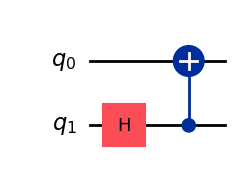
\includegraphics[width=0.35\textwidth]{circuito_bell.png}
    \caption{Circuito que prepara los estados de Bell. En el dibujo de Qiskit el qubit $q_0$ aparece arriba y corresponde al sistema de la \textbf{derecha} ($\mathsf{Y}$); la Hadamard y el control del CNOT actúan sobre $q_1$ ($\mathsf{X}$).}
    \label{fig:circuito_bell}
\end{figure}

\noindent El notebook comprueba también el aviso de la Sección 2.2 sobre el orden de los qubits en el CNOT:
\begin{lstlisting}
cx_cuaderno = np.array([[1,0,0,0],[0,1,0,0],[0,0,0,1],[0,0,1,0]])
qc01 = QuantumCircuit(2); qc01.cx(0, 1)
qc10 = QuantumCircuit(2); qc10.cx(1, 0)
print("cx(1,0) == CX del cuaderno:", np.allclose(Operator.from_circuit(qc10).data, cx_cuaderno))
print("cx(0,1) == CX del cuaderno:", np.allclose(Operator.from_circuit(qc01).data, cx_cuaderno))
print(np.real(Operator.from_circuit(qc01).data).astype(int))
\end{lstlisting}
\noindent La salida obtenida es:
\begin{lstlisting}[language={}]
cx(1,0) == CX del cuaderno: True
cx(0,1) == CX del cuaderno: False
[[1 0 0 0]
 [0 0 0 1]
 [0 0 1 0]
 [0 1 0 0]]
\end{lstlisting}
\noindent La matriz de \texttt{cx(0, 1)} intercambia las entradas $1$ y $3$, es decir, $|01\rangle\leftrightarrow|11\rangle$: cambia el bit izquierdo cuando el \textbf{derecho} vale $1$. Es el CNOT con el control en el qubit derecho. Un detalle más que merece atención: en los dibujos de circuitos de Qiskit el qubit $q_0$ aparece \textbf{arriba}, aunque en las cadenas y los vectores se escriba a la \textbf{derecha}.

\subsection{Experimento 5: mediciones parciales}

\noindent Para el estado $|\psi\rangle$ de \eqref{eq:psi2}, las probabilidades de medir solo $\mathsf{X}$ (qubit 1) o solo $\mathsf{Y}$ (qubit 0) se obtienen con \texttt{probabilities\_dict}:
\begin{lstlisting}
print("Probabilidades al medir X (qubit 1):", probs(psi, [1]))
print("Probabilidades al medir Y (qubit 0):", probs(psi, [0]))
\end{lstlisting}
\noindent La salida obtenida es:
\begin{lstlisting}[language={}]
Probabilidades al medir X (qubit 1): {'0': 0.6667, '1': 0.3333}
Probabilidades al medir Y (qubit 0): {'0': 0.6667, '1': 0.3333}
\end{lstlisting}
\noindent es decir, $\frac23$ y $\frac13$ en ambos casos, como en el cálculo a mano. Para los estados tras la medición, el notebook repite \texttt{psi.measure([q])} hasta obtener cada resultado y compara el estado resultante con el calculado a mano en la Sección 2.2:
\begin{lstlisting}
a_mano = {
    ("X", "0"): np.array([sqrt(3)/2, -1/2, 0, 0]),
    ("X", "1"): np.array([0, 0, 1j/sqrt(2), 1/sqrt(2)]),
    ("Y", "0"): np.array([sqrt(3)/2, 0, 1j/2, 0]),
    ("Y", "1"): np.array([0, -1/sqrt(2), 0, 1/sqrt(2)]),
}
qubit = {"X": 1, "Y": 0}
for (sistema, buscado), vec in a_mano.items():
    for _ in range(200):                   # repetimos hasta obtener ese resultado
        resultado, estado = psi.measure([qubit[sistema]])
        if resultado == buscado:
            break
    print(f"Medir {sistema}, resultado {resultado}: coincide con el cálculo a mano -> {estado.equiv(Statevector(vec))}")
\end{lstlisting}
\noindent Se usa \texttt{equiv} porque Qiskit puede devolver el estado multiplicado por una fase global (Experimento 3 de la Sección 1.3). La salida obtenida es:
\begin{lstlisting}[language={}]
Medir X, resultado 0: coincide con el cálculo a mano -> True
Medir X, resultado 1: coincide con el cálculo a mano -> True
Medir Y, resultado 0: coincide con el cálculo a mano -> True
Medir Y, resultado 1: coincide con el cálculo a mano -> True
\end{lstlisting}

\subsection{Experimento 6: GHZ frente a W}

\noindent Medimos el primer qubit (el de la izquierda, que es el qubit 2 de Qiskit) de los estados GHZ y W:
\begin{lstlisting}
ghz = Statevector(np.array([1, 0, 0, 0, 0, 0, 0, 1]) / sqrt(2))
w   = Statevector(np.array([0, 1, 1, 0, 1, 0, 0, 0]) / sqrt(3))
print(probs(ghz, [2]), probs(w, [2]))
for _ in range(5):
    r, e = ghz.measure([2])      # (y lo mismo con w)
\end{lstlisting}
\noindent Las probabilidades obtenidas son $\{0: 0.5,\ 1: 0.5\}$ para GHZ y $\{0: 0.6667,\ 1: 0.3333\}$ para W. Los resultados de cinco mediciones de cada uno fueron:
\begin{center}
\small\renewcommand{\arraystretch}{1.2}
\begin{tabular}{c|c|c||c|c}
& \multicolumn{2}{c||}{\textbf{GHZ}} & \multicolumn{2}{c}{\textbf{W}} \\
\textbf{Ejecución} & \textbf{Resultado} & \textbf{Estado final} & \textbf{Resultado} & \textbf{Estado final} \\ \hline
1 & $0$ & $|000\rangle$ & $0$ & $\frac{1}{\sqrt2}(|001\rangle + |010\rangle)$ \\
2 & $1$ & $|111\rangle$ & $0$ & $\frac{1}{\sqrt2}(|001\rangle + |010\rangle)$ \\
3 & $0$ & $|000\rangle$ & $1$ & $|100\rangle$ \\
4 & $0$ & $|000\rangle$ & $0$ & $\frac{1}{\sqrt2}(|001\rangle + |010\rangle)$ \\
5 & $0$ & $|000\rangle$ & $0$ & $\frac{1}{\sqrt2}(|001\rangle + |010\rangle)$
\end{tabular}
\end{center}
\noindent En GHZ, un solo resultado determina los tres qubits: queda $|000\rangle$ o $|111\rangle$. En W, si sale $0$ el estado queda en $\frac{1}{\sqrt2}(|001\rangle + |010\rangle) = |0\rangle|\psi^+\rangle$, con los otros dos qubits \textbf{todavía entrelazados}; si sale $1$ (probabilidad $\frac13$), queda en $|100\rangle$. Con solo cinco repeticiones las frecuencias ($4/5$ y $1/5$ en ambos casos) no tienen por qué coincidir con las probabilidades; para eso harían falta muchos más disparos, como en el Experimento 2 de la Sección 1.3.

\subsection{Experimento 7: estados reducidos}

\noindent La función \texttt{partial\_trace(estado, [0])} elimina el qubit 0 ($\mathsf{Y}$) y devuelve la matriz densidad de $\mathsf{X}$, es decir, el estado reducido correcto de la Sección 2.2:
\begin{lstlisting}
for etiqueta, nombre in [("00", "phi+"), ("01", "psi+"), ("10", "phi-"), ("11", "psi-")]:
    b = Statevector.from_label(etiqueta).evolve(bell_circ)
    rho_X = partial_trace(b, [0]).data
    print(f"Estado reducido de X en |{nombre}>:")
    print(np.round(rho_X, 4))
\end{lstlisting}
\noindent Para los cuatro estados de Bell la salida es la misma matriz,
\begin{lstlisting}[language={}]
[[0.5+0.j 0. +0.j]
 [0. +0.j 0.5+0.j]]
\end{lstlisting}
\noindent es decir,
\[ \rho_{\mathsf{X}} = \begin{pmatrix} 0.5 & 0 \\ 0 & 0.5\end{pmatrix} = \tfrac12\mathbb{I}. \]
(El \texttt{+0.j} indica que NumPy trabaja con números complejos, aunque aquí la parte imaginaria sea nula.) Esto confirma que $\mathsf{X}$ se comporta igual en los cuatro estados (como un bit completamente aleatorio), mientras que la fórmula ingenua daría $|+\rangle$ para $|\psi^+\rangle$ y $|-\rangle$ para $|\psi^-\rangle$, que son distinguibles.

\subsection{Experimento 8: operaciones de dos qubits}

\noindent Por último, se comprueban cuatro hechos sobre operaciones:
\begin{itemize}
    \item $H\otimes\mathbb{I}\otimes X$ es unitaria ($U^\dagger U = \mathbb{I}_8$), como garantiza la proposición sobre productos tensoriales de unitarias.
    \item $CZ$ es simétrico: \texttt{cz(0, 1)} y \texttt{cz(1, 0)} tienen la misma matriz.
    \item $CZ = (\mathbb{I}\otimes H)\,CX\,(\mathbb{I}\otimes H)$, consecuencia de $HXH = Z$.
    \item El SWAP se obtiene con \textbf{tres CNOT} alternando el control:
    \[ \mathrm{SWAP} = CX_{1\to0}\,CX_{0\to1}\,CX_{1\to0} \]
    (lo que también puede comprobarse a mano multiplicando las tres matrices de permutación).
\end{itemize}
\begin{lstlisting}
H, I, X = Operator.from_label("H"), Operator.from_label("I"), Operator.from_label("X")
U = (H ^ I ^ X).data
print("H⊗I⊗X unitaria:", np.allclose(U.conj().T @ U, np.eye(8)))

cz01 = QuantumCircuit(2); cz01.cz(0, 1)
cz10 = QuantumCircuit(2); cz10.cz(1, 0)
print("CZ simétrico:", Operator.from_circuit(cz01).equiv(Operator.from_circuit(cz10)))

cz_desde_cx = QuantumCircuit(2)
cz_desde_cx.h(0); cz_desde_cx.cx(1, 0); cz_desde_cx.h(0)
print("CZ = (I⊗H) CX (I⊗H):", Operator.from_circuit(cz_desde_cx).equiv(Operator.from_circuit(cz10)))

swap_3cx = QuantumCircuit(2)
swap_3cx.cx(1, 0); swap_3cx.cx(0, 1); swap_3cx.cx(1, 0)
swap_q = QuantumCircuit(2); swap_q.swap(0, 1)
print("SWAP = tres CNOT:", Operator.from_circuit(swap_3cx).equiv(Operator.from_circuit(swap_q)))
\end{lstlisting}
\noindent La salida obtenida es:
\begin{lstlisting}[language={}]
H⊗I⊗X unitaria: True
CZ simétrico: True
CZ = (I⊗H) CX (I⊗H): True
SWAP = tres CNOT: True
\end{lstlisting}

\begin{figure}[htbp]
    \centering
    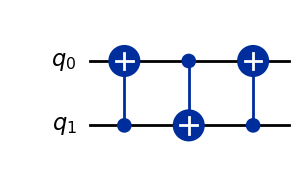
\includegraphics[width=0.35\textwidth]{circuito_swap.png}
    \caption{El SWAP construido con tres CNOT alternando el control. De nuevo, $q_0$ (arriba) es el qubit de la derecha: el primer y el tercer CNOT tienen el control en $q_1$ ($CX_{1\to0}$) y el segundo en $q_0$ ($CX_{0\to1}$).}
    \label{fig:circuito_swap}
\end{figure}


\providecommand{\pasoguiado}[3]{%
\begin{tcolorbox}[colback=gray!6!white,colframe=gray!55!black,fonttitle=\bfseries,title={#1}]
#2
\tcblower
\small #3
\end{tcolorbox}}

\cleardoublepage
\section{Resumen: un ejemplo guiado}

\noindent Alicia tiene un bit (el sistema $\mathsf{X}$) y Bruno otro (el sistema $\mathsf{Y}$). Primero son monedas (caso clásico) y después qubits (caso cuántico). Escribimos siempre a Alicia a la izquierda.

\subsection{Parte 1: dos monedas}

\pasoguiado{Paso 1. ¿Qué resultados puede haber?}
{$00,\quad 01,\quad 10,\quad 11$.}
{\textbf{Producto cartesiano:} los estados del sistema conjunto son las parejas de $\{0,1\}\times\{0,1\}$, ordenadas como en un diccionario (o como números en binario). Con $n$ bits hay $2^n$ estados.}

\pasoguiado{Paso 2. Cada uno lanza su moneda, por separado}
{Alicia: $\left(\frac14,\frac34\right)$. \quad Bruno: $\left(\frac23,\frac13\right)$.
\[ \begin{pmatrix}1/4\\3/4\end{pmatrix}\otimes\begin{pmatrix}2/3\\1/3\end{pmatrix} = \begin{pmatrix}\frac14\cdot\frac23\\[0.5mm]\frac14\cdot\frac13\\[0.5mm]\frac34\cdot\frac23\\[0.5mm]\frac34\cdot\frac13\end{pmatrix} = \begin{pmatrix}1/6\\1/12\\1/2\\1/4\end{pmatrix}. \]}
{\textbf{Producto tensorial:} se copia el vector de Bruno una vez por cada entrada de Alicia, multiplicado por esa entrada. \textbf{Independencia:} si los sistemas no tienen nada que ver, el vector conjunto es el producto tensorial de los individuales (\textbf{estado producto}).}

\pasoguiado{Paso 3. ¿Cómo sé si son independientes?}
{\[ \begin{pmatrix}p_{00}&p_{01}\\p_{10}&p_{11}\end{pmatrix} = \begin{pmatrix}1/6&1/12\\1/2&1/4\end{pmatrix}, \qquad \tfrac16\cdot\tfrac14 - \tfrac1{12}\cdot\tfrac12 = \tfrac1{24} - \tfrac1{24} = 0. \]}
{\textbf{Criterio del rango:} determinante $0$ (rango $1$) $\iff$ independientes. En un producto, las filas son proporcionales (aquí la segunda es $3$ veces la primera).}

\pasoguiado{Paso 4. Alicia mira su moneda, Bruno no}
{Alicia ve $0$ (prob.\ $\frac16 + \frac1{12} = \frac14$): Bruno $= \left(\frac16, \frac1{12}\right)\big/\frac14 = \left(\frac23, \frac13\right)$. \\
Alicia ve $1$ (prob.\ $\frac12 + \frac14 = \frac34$): Bruno $= \left(\frac12, \frac14\right)\big/\frac34 = \left(\frac23, \frac13\right)$.}
{\textbf{Medición parcial:} (1) separar los casos según lo que ve Alicia; (2) sumar para obtener la probabilidad; (3) dividir por esa suma. Con independencia, \textbf{mirar a Alicia no dice nada sobre Bruno}.}

\pasoguiado{Paso 5. El CNOT crea correlación}
{``Si Alicia tiene $1$, Bruno da la vuelta'': se intercambian las entradas de $10$ y $11$.
\[ \begin{pmatrix}1/6\\1/12\\1/2\\1/4\end{pmatrix} \xrightarrow{\text{CNOT}} \begin{pmatrix}1/6\\1/12\\1/4\\1/2\end{pmatrix}, \qquad \tfrac16\cdot\tfrac12 - \tfrac1{12}\cdot\tfrac14 = \tfrac{3}{48} \neq 0. \]
Alicia ve $0$: Bruno $= \left(\frac23,\frac13\right)$. \quad Alicia ve $1$: Bruno $= \left(\frac13,\frac23\right)$.}
{\textbf{Correlación} = falta de independencia: mirar un sistema informa sobre el otro. El \textbf{CNOT no es una operación independiente} (lo que le pasa a Bruno depende de Alicia), y por eso puede \textbf{crear} correlación.}

\pasoguiado{Paso 6. Una operación que no crea correlación}
{NOT solo a Alicia ($X\otimes\mathbb{I}$): \quad $\begin{pmatrix}1/6\\1/12\\1/2\\1/4\end{pmatrix} \to \begin{pmatrix}1/2\\1/4\\1/6\\1/12\end{pmatrix} = \begin{pmatrix}3/4\\1/4\end{pmatrix}\otimes\begin{pmatrix}2/3\\1/3\end{pmatrix}$.}
{\textbf{Operaciones independientes = producto tensorial de matrices} ($M\otimes N$; ``no hacer nada'' es $\mathbb{I}$). Una operación así \textbf{nunca crea correlación}.}

\subsection{Parte 2: dos qubits}

\pasoguiado{Paso 7. Alicia en $|+\rangle$, Bruno en $|0\rangle$}
{\[ \begin{pmatrix}1/\sqrt2\\1/\sqrt2\end{pmatrix}\otimes\begin{pmatrix}1\\0\end{pmatrix} = \begin{pmatrix}1/\sqrt2\\0\\1/\sqrt2\\0\end{pmatrix} = \tfrac{1}{\sqrt2}|00\rangle + \tfrac{1}{\sqrt2}|10\rangle, \qquad \tfrac12 + \tfrac12 = 1. \]}
{\textbf{Estado producto cuántico.} Es un estado válido porque \textbf{la norma del producto tensorial es el producto de las normas} ($1\cdot1 = 1$), consecuencia de que el producto interno es multiplicativo.}

\pasoguiado{Paso 8. El CNOT entrelaza}
{\[ \begin{pmatrix}1/\sqrt2\\0\\1/\sqrt2\\0\end{pmatrix} \xrightarrow{\text{CNOT}} \begin{pmatrix}1/\sqrt2\\0\\0\\1/\sqrt2\end{pmatrix} = |\phi^+\rangle, \qquad \tfrac{1}{\sqrt2}\cdot\tfrac{1}{\sqrt2} - 0\cdot0 = \tfrac12 \neq 0. \]}
{\textbf{Entrelazamiento:} un estado que no es producto (versión cuántica de la correlación). El CNOT entrelaza \textbf{cuando el control está en superposición}: hace a la vez ``no tocar a Bruno'' y ``darle la vuelta''. $|\phi^+\rangle$ es un \textbf{estado de Bell}, y ``$H$ y después CNOT'' es la receta estándar para fabricarlo.}

\pasoguiado{Paso 9. Alicia mide su qubit}
{$|\phi^+\rangle = |0\rangle\otimes\left(\tfrac{1}{\sqrt2}|0\rangle\right) + |1\rangle\otimes\left(\tfrac{1}{\sqrt2}|1\rangle\right)$. \\
Alicia ve $0$ (prob.\ $\frac12$): Bruno queda en $|0\rangle$. \quad Alicia ve $1$ (prob.\ $\frac12$): Bruno queda en $|1\rangle$.}
{\textbf{Medición parcial cuántica:} la misma receta, cambiando ``sumar probabilidades'' por ``sumar módulos al cuadrado'' y ``dividir por la suma'' por ``dividir por la norma''. Los dos qubits \textbf{siempre coinciden}.}

\pasoguiado{Paso 10. Lo que el mundo clásico no puede hacer}
{Aplicamos $H\otimes H$. \\
\textit{Monedas coincidentes} (mitad $|00\rangle$, mitad $|11\rangle$): $|00\rangle\to|{+}{+}\rangle$ y $|11\rangle\to|{-}{-}\rangle$ dan los cuatro resultados con probabilidad $\frac14$. \textbf{La correlación desaparece.}
\textit{Estado entrelazado:}
\begin{align*} (H\otimes H)|\phi^+\rangle &= \tfrac{1}{\sqrt2}\Big[\tfrac12(|00\rangle{+}|01\rangle{+}|10\rangle{+}|11\rangle) + \tfrac12(|00\rangle{-}|01\rangle{-}|10\rangle{+}|11\rangle)\Big] \\ &= \tfrac{1}{\sqrt2}|00\rangle + \tfrac{1}{\sqrt2}|11\rangle = |\phi^+\rangle. \end{align*}
Los términos $|01\rangle$ y $|10\rangle$ se cancelan: \textbf{siguen coincidiendo siempre}.}
{\textbf{El entrelazamiento no es simplemente correlación clásica}: dos situaciones con las mismas probabilidades al medir directamente se comportan distinto tras aplicar puertas, por \textbf{interferencia}. Es la idea de $|+\rangle$ frente a $|-\rangle$, ahora con dos qubits.}

\begin{center}
\small\renewcommand{\arraystretch}{1.15}
\begin{tabular}{c|l|l}
\textbf{Paso} & \textbf{Qué hicimos} & \textbf{Concepto} \\ \hline
1 & Listar $00, 01, 10, 11$ & Producto cartesiano, orden \\
2 & Multiplicar probabilidades & Producto tensorial = independencia \\
3 & Determinante $= 0$ & Criterio del rango \\
4 & Alicia mira; Bruno no cambia & Medición parcial; independencia \\
5 & CNOT; Bruno sí cambia & Correlación; el CNOT no es ``independiente'' \\
6 & NOT solo a Alicia & $X\otimes\mathbb{I}$ no crea correlación \\
7 & $|+\rangle\otimes|0\rangle$ & Estado producto cuántico; norma multiplicativa \\
8 & CNOT $\to|\phi^+\rangle$ & Entrelazamiento; estados de Bell \\
9 & Alicia mide & Medición parcial cuántica \\
10 & $H\otimes H$ & Entrelazamiento $\neq$ correlación clásica
\end{tabular}
\end{center}

\noindent \textbf{Conexión con el TFG:} el mapa de características de Havlíček et al.\ \cite{havlicek2019supervised} hace a gran escala lo de los pasos 7 y 8: pone los qubits en superposición con puertas de Hadamard y los entrelaza con CNOT. Sin el paso 8, los estados serían productos (paso 7) y el kernel se factorizaría y podría calcularse con un ordenador clásico.


\chapter{Circuitos cuánticos}

\noindent En este capítulo se introduce el \textbf{modelo de circuito cuántico}, el lenguaje en el que se escriben los algoritmos cuánticos (y los mapas de características de los kernels cuánticos). Después se desarrollan las herramientas matemáticas necesarias para analizarlos (productos internos, proyecciones y mediciones proyectivas) y se estudian tres limitaciones fundamentales de la información cuántica: la irrelevancia de las fases globales, el teorema de no clonación y la imposibilidad de distinguir estados no ortogonales.
\cleardoublepage
\section{Circuitos}

\noindent En informática, un \textbf{circuito} es un modelo de cálculo en el que la información viaja por \textbf{cables} (o hilos) a través de una red de \textbf{puertas}, que representan operaciones sobre esa información. Los \textbf{circuitos cuánticos} son un caso particular de esta idea general, y son el lenguaje en el que se escriben los algoritmos cuánticos y, en particular, los mapas de características de este trabajo.

\noindent Aunque la palabra ``circuito'' sugiere una trayectoria circular, en los modelos de computación que estudiaremos \textbf{no se permiten ciclos}: los circuitos son \textbf{acíclicos}. La información fluye siempre de izquierda a derecha, y un circuito representa una \textbf{secuencia finita de operaciones} sin bucles de realimentación. Esto garantiza que el cálculo termina y que se puede evaluar puerta a puerta.

\subsection{Circuitos booleanos}

\noindent En un \textbf{circuito booleano} (clásico), los cables transportan valores binarios ($0$ o $1$) y las puertas son operaciones lógicas. Las más habituales son:
\[
\begin{array}{c|c}
a & \neg a \\ \hline 0 & 1 \\ 1 & 0
\end{array}
\qquad\qquad
\begin{array}{c|c}
ab & a\wedge b \\ \hline 00 & 0\\ 01 & 0 \\ 10 & 0 \\ 11 & 1
\end{array}
\qquad\qquad
\begin{array}{c|c}
ab & a\vee b \\ \hline 00 & 0\\ 01 & 1 \\ 10 & 1 \\ 11 & 1
\end{array}
\qquad\qquad
\begin{array}{c|c}
ab & a\oplus b \\ \hline 00 & 0\\ 01 & 1 \\ 10 & 1 \\ 11 & 0
\end{array}
\]
Son, respectivamente, \textbf{NOT} ($\neg$), \textbf{AND} ($\wedge$), \textbf{OR} ($\vee$) y el \textbf{OR exclusivo} o \textbf{XOR} ($\oplus$), que vale $1$ cuando exactamente una de las entradas vale $1$. Obsérvese que $a\oplus b$ es la \textbf{suma módulo $2$}, el mismo símbolo que apareció en el CNOT: $CX|a\rangle|b\rangle = |a\rangle|a\oplus b\rangle$.

\noindent Además de estas puertas, hay una operación que en los circuitos clásicos suele darse por supuesta: el \textbf{fan-out} (representado con un punto sobre el cable), que \textbf{copia} el valor de un cable para poder usarlo como entrada de varias puertas. En el mundo clásico copiar es trivial; veremos (Sección~3.3) que en el mundo cuántico es \textbf{imposible} copiar un estado arbitrario. Por eso, al traducir circuitos booleanos a cuánticos, el fan-out debe tratarse explícitamente como una puerta más.

\begin{tcolorbox}[colback=cyan!5!white,colframe=cyan!75!black,title=\textbf{Ejemplo: Un circuito que calcula el XOR}]
El siguiente circuito, con entradas $\mathsf{X}$ e $\mathsf{Y}$, usa dos fan-out, dos NOT, dos AND y un OR:
\begin{center}
\begin{tikzpicture}[x=1cm,y=0.8cm,
  puerta/.style={draw,fill=blue!25,minimum size=0.7cm,inner sep=1pt}]
  \node (Y) at (0,3) {$\mathsf{Y}$};
  \node (X) at (0,0) {$\mathsf{X}$};
  \fill (1,3) circle (2pt); \fill (1,0) circle (2pt);
  \draw (Y) -- (1,3); \draw (X) -- (1,0);
  \node[puerta] (n1) at (2.5,2.3) {$\neg$};
  \node[puerta] (n2) at (2.5,0.7) {$\neg$};
  \node[puerta] (a1) at (5,2.8) {$\wedge$};
  \node[puerta] (a2) at (5,0.2) {$\wedge$};
  \node[puerta] (o)  at (7,1.5) {$\vee$};
  \draw (1,3) |- (4.65,3.0);
  \draw (1,3) |- (n1.west);
  \draw (1,0) |- (n2.west);
  \draw (1,0) |- (4.65,0.0);
  \draw (n2.east) -- (3.3,0.7) |- (4.65,2.6);
  \draw (n1.east) -- (3.6,2.3) |- (4.65,0.4);
  \draw (a1.east) -- (6,2.8) |- (6.65,1.65);
  \draw (a2.east) -- (6,0.2) |- (6.65,1.35);
  \draw (o.east) -- (8,1.5) node[right] {salida};
\end{tikzpicture}
\end{center}
La puerta AND superior recibe $\mathsf{Y}$ y $\neg\mathsf{X}$; la inferior, $\neg\mathsf{Y}$ y $\mathsf{X}$. La salida es
\[ (\mathsf{Y}\wedge\neg\mathsf{X}) \vee (\neg\mathsf{Y}\wedge\mathsf{X}), \]
que vale $1$ exactamente cuando una y solo una de las entradas es $1$. Comprobándolo para las cuatro entradas:
\begin{center}
\begin{tabular}{cc|cc|c}
$\mathsf{X}$ & $\mathsf{Y}$ & $\mathsf{Y}\wedge\neg\mathsf{X}$ & $\neg\mathsf{Y}\wedge\mathsf{X}$ & salida \\ \hline
0 & 0 & 0 & 0 & 0 \\
0 & 1 & 1 & 0 & 1 \\
1 & 0 & 0 & 1 & 1 \\
1 & 1 & 0 & 0 & 0
\end{tabular}
\end{center}
que es exactamente la tabla de $\mathsf{X}\oplus\mathsf{Y}$.
\end{tcolorbox}

\subsection{Otros tipos de circuitos}

\noindent La noción de circuito es muy general. En los \textbf{circuitos aritméticos}, los cables transportan números (por ejemplo, enteros) y las puertas son operaciones aritméticas como la suma ($+$) y el producto ($*$). Por ejemplo, con entradas $x$, $y$ y una tercera entrada fija igual a $1$:
\begin{itemize}
    \item un fan-out de $x$ y una puerta $*$ calculan $x\cdot x = x^2$;
    \item una puerta $+$ calcula $x^2 + y$;
    \item otra puerta $+$ calcula $y + 1$;
    \item una última puerta $*$ calcula $(x^2+y)(y+1) = x^2y + x^2 + y^2 + y$.
\end{itemize}
También hay \textbf{circuitos probabilísticos}, cuyas puertas representan operaciones probabilísticas (matrices estocásticas). Los circuitos cuánticos son el análogo con operaciones unitarias.

\subsection{Circuitos cuánticos}

\noindent En el modelo de circuito cuántico, \textbf{los cables representan qubits} y \textbf{las puertas representan operaciones} sobre ellos. Por ahora, las operaciones permitidas son las que conocemos: \textbf{operaciones unitarias} y \textbf{mediciones en la base estándar}.

\paragraph{Un qubit}\mbox{}\\

\noindent El circuito más sencillo tiene un solo cable (un qubit, llamado $\mathsf{X}$) y una secuencia de puertas de un qubit:
\begin{center}
\begin{quantikz}
\lstick{$\mathsf{X}$} & \gate{H} & \gate{S} & \gate{H} & \gate{T} &
\end{quantikz}
\end{center}
La información fluye de izquierda a derecha: primero se aplica $H$, después $S$, después $H$ y por último $T$. Por tanto, el circuito completo aplica la operación
\[ T\,H\,S\,H. \]

\begin{tcolorbox}[colback=blue!5!white,colframe=blue!75!black,title=\textbf{Nota Aclaratoria: El circuito se lee al revés que la fórmula}]
En el circuito, la primera puerta está a la \textbf{izquierda}; en el producto de matrices, la primera operación está a la \textbf{derecha}, porque es la que actúa primero sobre el vector: $THSH|\psi\rangle = T\big(H\big(S\big(H|\psi\rangle\big)\big)\big)$. Así, el circuito $H \to S \to H \to T$ corresponde a la matriz $THSH$. Es la regla de composición de la Sección~1.2 (y, para matrices estocásticas, de la Sección~1.1), ahora con una representación gráfica.
\end{tcolorbox}

\noindent A veces se indican explícitamente los estados de entrada y de salida. Es habitual que todos los qubits empiecen en $|0\rangle$:
\begin{center}
\begin{quantikz}
\lstick{$|0\rangle$} & \gate{H} & \gate{S} & \gate{H} & \gate{T} & \rstick{$\frac{1+i}{2}|0\rangle + \frac{1}{\sqrt2}|1\rangle$}
\end{quantikz}
\end{center}
\noindent Comprobémoslo paso a paso:
\begin{align*}
|0\rangle &\xrightarrow{H} \tfrac{1}{\sqrt2}|0\rangle + \tfrac{1}{\sqrt2}|1\rangle
\xrightarrow{S} \tfrac{1}{\sqrt2}|0\rangle + \tfrac{i}{\sqrt2}|1\rangle
\xrightarrow{H} \tfrac{1}{\sqrt2}\cdot\tfrac{1}{\sqrt2}\big(|0\rangle + |1\rangle\big) + \tfrac{i}{\sqrt2}\cdot\tfrac{1}{\sqrt2}\big(|0\rangle - |1\rangle\big) \\
&= \tfrac{1+i}{2}|0\rangle + \tfrac{1-i}{2}|1\rangle
\xrightarrow{T} \tfrac{1+i}{2}|0\rangle + \tfrac{1-i}{2}\cdot\tfrac{1+i}{\sqrt2}|1\rangle = \tfrac{1+i}{2}|0\rangle + \tfrac{1}{\sqrt2}|1\rangle,
\end{align*}
donde en el último paso se ha usado $(1-i)(1+i) = 2$. Como comprobación, $\left|\frac{1+i}{2}\right|^2 + \left|\frac{1}{\sqrt2}\right|^2 = \frac12 + \frac12 = 1$.

\paragraph{Varios qubits y la convención de orden}\mbox{}\\

\noindent Con varios qubits, cada uno tiene su cable horizontal. Por ejemplo, el siguiente circuito actúa sobre dos qubits $\mathsf{X}$ e $\mathsf{Y}$: aplica una Hadamard a $\mathsf{Y}$ y después un CNOT, cuyo \textbf{control} (el punto relleno) es $\mathsf{Y}$ y cuyo \textbf{objetivo} (el símbolo $\oplus$) es $\mathsf{X}$:
\begin{center}
\begin{quantikz}
\lstick{$\mathsf{Y}$} & \gate{H} & \ctrl{1} & \\
\lstick{$\mathsf{X}$} & & \targ{} &
\end{quantikz}
\end{center}
Antes de interpretarlo hay que saber \textbf{en qué orden se leen los cables}.

\begin{tcolorbox}[colback=teal!5!white,colframe=teal!75!black,title=\textbf{Convención de Qiskit para ordenar los qubits en un circuito}]
El qubit situado \textbf{más arriba} en el diagrama tiene índice $0$ y corresponde a la posición \textbf{más a la derecha} de la tupla, la cadena o el producto tensorial. El segundo desde arriba tiene índice $1$ y corresponde a la segunda posición desde la derecha, y así sucesivamente. Es decir, con $n$ qubits $(\mathsf{q}_{n-1},\dots,\mathsf{q}_0)$:
\begin{align*} \text{cable de arriba} &= \mathsf{q}_0 = \text{factor de la derecha}, \\ \text{cable de abajo} &= \mathsf{q}_{n-1} = \text{factor de la izquierda}. \end{align*}
En otras palabras, \textbf{leer los cables de abajo arriba equivale a leer la tupla de izquierda a derecha}. Esta convención es la inversa de la de muchos libros (donde el cable de arriba es el de la izquierda), y es una fuente frecuente de errores. Es la misma que ya vimos para las cadenas en el Capítulo~2, trasladada a los dibujos.
\end{tcolorbox}

\noindent En el circuito anterior, $\mathsf{X}$ está abajo e $\mathsf{Y}$ arriba, así que el par se ordena como $(\mathsf{X},\mathsf{Y})$, igual que en el Capítulo~2. Si la entrada es $|\psi\rangle\otimes|\phi\rangle$, el qubit de abajo, $\mathsf{X}$, empieza en $|\psi\rangle$, y el de arriba, $\mathsf{Y}$, en $|\phi\rangle$.

\paragraph{Del circuito a la matriz, paso a paso}\mbox{}\\

\noindent Recorremos el circuito de izquierda a derecha, traduciendo cada ``columna'' de puertas en una matriz $4\times4$.

\noindent \textbf{1. Hadamard sobre $\mathsf{Y}$.} Cuando una puerta actúa sobre un solo qubit, a los demás no les pasa nada, es decir, se les aplica la identidad. Como $\mathsf{Y}$ es el factor de la \textbf{derecha}, la operación es
\[
\mathbb{I}\otimes H = \begin{pmatrix} H & 0 \\ 0 & H\end{pmatrix} = \frac{1}{\sqrt2}\begin{pmatrix} 1&1&0&0\\1&-1&0&0\\0&0&1&1\\0&0&1&-1\end{pmatrix}.
\]
Obsérvese que es $\mathbb{I}\otimes H$ y \textbf{no} $H\otimes\mathbb{I}$: la $H$ va a la derecha porque actúa sobre el cable de arriba.

\noindent \textbf{2. CNOT con control $\mathsf{Y}$ y objetivo $\mathsf{X}$.} Actúa como $|b\rangle_{\mathsf{Y}}|a\rangle_{\mathsf{X}} \mapsto |b\rangle_{\mathsf{Y}}|a\oplus b\rangle_{\mathsf{X}}$. Escrito en el orden $(\mathsf{X},\mathsf{Y})$, es decir, $|ab\rangle\mapsto|(a\oplus b)\,b\rangle$:
\[
|00\rangle\mapsto|00\rangle,\quad |01\rangle\mapsto|11\rangle,\quad |10\rangle\mapsto|10\rangle,\quad |11\rangle\mapsto|01\rangle,
\qquad
\begin{pmatrix} 1&0&0&0\\0&0&0&1\\0&0&1&0\\0&1&0&0\end{pmatrix}.
\]
Es el CNOT con el control en el qubit \textbf{derecho}, distinto del $CX$ del Capítulo~2 (que tenía el control a la izquierda). Lo denotaremos $\mathrm{CNOT}_{\mathsf{Y}\to\mathsf{X}}$.

\noindent \textbf{3. Composición.} La operación del circuito completo es el producto, con la primera operación a la derecha:
\[
U = \begin{pmatrix} 1&0&0&0\\0&0&0&1\\0&0&1&0\\0&1&0&0\end{pmatrix}
\frac{1}{\sqrt2}\begin{pmatrix} 1&1&0&0\\1&-1&0&0\\0&0&1&1\\0&0&1&-1\end{pmatrix}
= \frac{1}{\sqrt2}\begin{pmatrix} 1&1&0&0\\0&0&1&-1\\0&0&1&1\\1&-1&0&0\end{pmatrix}.
\]
(Multiplicar por esa matriz de permutación a la izquierda simplemente \textbf{reordena las filas}: la fila $2$ del resultado es la fila $4$ del segundo factor, y la fila $4$ es la fila $2$.)

\noindent \textbf{4. Lectura del resultado.} Las columnas de $U$ son las imágenes de la base estándar:
\[
U|00\rangle = |\phi^+\rangle, \qquad U|01\rangle = |\phi^-\rangle, \qquad U|10\rangle = |\psi^+\rangle, \qquad U|11\rangle = -|\psi^-\rangle.
\]
Por ejemplo, la primera columna es $\frac{1}{\sqrt2}(1,0,0,1)^T = \frac{1}{\sqrt2}(|00\rangle + |11\rangle)$. Así, este circuito \textbf{transforma la base estándar en la base de Bell}, y en particular, partiendo de $|00\rangle$, \textbf{fabrica el estado de Bell $|\phi^+\rangle$}.

\begin{tcolorbox}[colback=blue!5!white,colframe=blue!75!black,title=\textbf{Nota Aclaratoria: El signo menos de $-|\psi^-\rangle$}]
El signo de $U|11\rangle = -|\psi^-\rangle$ es una \textbf{fase global} de ese estado de salida: $-|\psi^-\rangle$ y $|\psi^-\rangle$ representan el mismo estado físico (Sección~3.3). Aun así, si se quiere que $U$ lleve exactamente la base estándar en la base de Bell, puede eliminarse sin afectar a las otras tres columnas, por ejemplo añadiendo una puerta $CZ$ al principio (que solo cambia el signo de $|11\rangle$) o una puerta SWAP al final (que solo intercambia las amplitudes de $|01\rangle$ y $|10\rangle$, y así $-|\psi^-\rangle = \frac{1}{\sqrt2}(-|01\rangle + |10\rangle)$ pasa a ser $|\psi^-\rangle$, mientras que $|\phi^\pm\rangle$ y $|\psi^+\rangle$ no cambian).

Compárese con el Capítulo~2, donde el circuito $CX(H\otimes\mathbb{I})$ ponía la Hadamard y el control en el qubit \textbf{izquierdo}: allí $|01\rangle\mapsto|\psi^+\rangle$ y $|10\rangle\mapsto|\phi^-\rangle$. Al cambiar qué qubit hace de control, cambia qué estado de la base estándar va a cada estado de Bell. Es otra muestra de que el orden de los qubits importa.
\end{tcolorbox}

\paragraph{Mediciones y bits clásicos}\mbox{}\\

\noindent Un circuito cuántico también puede contener \textbf{cables de bits clásicos}, que se dibujan con \textbf{líneas dobles}, y \textbf{puertas de medición}, que se dibujan con un medidor (una aguja sobre un arco):
\begin{center}
\begin{quantikz}
\lstick{$\mathsf{Y}$} & \gate{H} & \ctrl{1} & \meter{} & \setwiretype{c} \rstick{$\mathsf{B}$} \\
\lstick{$\mathsf{X}$} & & \targ{} & \meter{} & \setwiretype{c} \rstick{$\mathsf{A}$}
\end{quantikz}
\end{center}
Cada medición es una medición en la base estándar del qubit correspondiente, y su resultado se escribe en un bit clásico ($\mathsf{A}$ para $\mathsf{X}$ y $\mathsf{B}$ para $\mathsf{Y}$). En este dibujo, la medición se representa como una puerta que \textbf{recibe un qubit y devuelve un bit clásico}: el qubit medido se \textbf{descarta} y puede ignorarse a partir de ese momento (tras la medición está en $|0\rangle$ o $|1\rangle$, y toda su información ha pasado al bit clásico). Otra forma equivalente de dibujarlo es mantener los cables de los qubits y añadir aparte los cables clásicos, con flechas desde cada medidor hasta el bit donde se \textbf{sobrescribe} el resultado.

\noindent En este ejemplo concreto, el estado antes de medir es $|\phi^+\rangle = \frac{1}{\sqrt2}(|00\rangle + |11\rangle)$, así que se obtiene $\mathsf{AB} = 00$ o $11$, cada uno con probabilidad $\frac12$: los dos bits clásicos siempre coinciden.

\begin{tcolorbox}[colback=teal!5!white,colframe=teal!75!black,title=\textbf{Conexión con el TFG: cómo se estima un kernel cuántico}]
Este es exactamente el tipo de circuito que se usa para estimar un kernel cuántico. Si $U(\mathbf{x})$ es el circuito que codifica el dato $\mathbf{x}$, el circuito
\begin{center}
\begin{quantikz}
\lstick{$|0\rangle^{\otimes n}$} & \gate{U(\mathbf{y})} & \gate{U(\mathbf{x})^\dagger} & \meter{} & \setwiretype{c}
\end{quantikz}
\end{center}
prepara el estado $U(\mathbf{x})^\dagger U(\mathbf{y})|0\cdots0\rangle$ y lo mide. La probabilidad de obtener $0\cdots0$ es
\[ \big|\langle 0\cdots0|U(\mathbf{x})^\dagger U(\mathbf{y})|0\cdots0\rangle\big|^2 = |\langle\phi(\mathbf{x})|\phi(\mathbf{y})\rangle|^2 = K(\mathbf{x},\mathbf{y}), \]
usando $\langle 0\cdots0|U(\mathbf{x})^\dagger = \big(U(\mathbf{x})|0\cdots0\rangle\big)^\dagger = \langle\phi(\mathbf{x})|$. Repitiendo el circuito $N$ veces y contando la frecuencia del resultado $0\cdots0$ se estima el kernel, con un error del orden de $1/\sqrt N$ (Sección~1.3).
\end{tcolorbox}

\subsection{Símbolos de las puertas más habituales}

\noindent Para leer circuitos conviene conocer los símbolos estándar:
\begin{itemize}
    \item \textbf{Puertas de un qubit:} un cuadrado con la letra de la operación.
    \begin{center}
    \begin{quantikz}[column sep=0.3cm] & \gate{X} & \end{quantikz}\;
    \begin{quantikz}[column sep=0.3cm] & \gate{Y} & \end{quantikz}\;
    \begin{quantikz}[column sep=0.3cm] & \gate{Z} & \end{quantikz}\;
    \begin{quantikz}[column sep=0.3cm] & \gate{H} & \end{quantikz}\;
    \begin{quantikz}[column sep=0.3cm] & \gate{S} & \end{quantikz}\;
    \begin{quantikz}[column sep=0.3cm] & \gate{T} & \end{quantikz}
    \end{center}
    La puerta NOT ($X$) también se dibuja a veces como un círculo con un signo más, \begin{quantikz}[column sep=0.3cm] & \targ{} & \end{quantikz}, el mismo símbolo que el objetivo de un CNOT (lo cual tiene sentido: el CNOT aplica un $X$ al objetivo).
    \item \textbf{SWAP:} dos aspas unidas por una línea vertical:
    \begin{center}
    \begin{quantikz}[row sep=0.3cm] & \swap{1} & \\ & \targX{} & \end{quantikz}
    \end{center}
    \item \textbf{Puertas controladas:} un \textbf{punto relleno} (el control) unido por una línea vertical a la operación que se controla. De izquierda a derecha: CNOT, Toffoli (dos controles) y Fredkin (SWAP controlado):
    \begin{center}
    \begin{quantikz}[row sep=0.3cm] & \ctrl{1} & \\ & \targ{} & \end{quantikz}
    \qquad
    \begin{quantikz}[row sep=0.3cm] & \ctrl{1} & \\ & \ctrl{1} & \\ & \targ{} & \end{quantikz}
    \qquad
    \begin{quantikz}[row sep=0.3cm] & \ctrl{1} & \\ & \swap{1} & \\ & \targX{} & \end{quantikz}
    \end{center}
    \item \textbf{Operaciones arbitrarias:} cualquier unitaria sobre varios qubits puede verse como una puerta, que se dibuja como un rectángulo con su nombre que abarca todos los cables sobre los que actúa. Su versión controlada añade un punto de control:
    \begin{center}
    \begin{quantikz}[row sep=0.25cm] & \gate[3]{U} & \\ & & \\ & & \end{quantikz}
    \qquad\qquad
    \begin{quantikz}[row sep=0.25cm] & \ctrl{1} & \\ & \gate[3]{U} & \\ & & \\ & & \end{quantikz}
    \end{center}
\end{itemize}

\begin{tcolorbox}[colback=teal!5!white,colframe=teal!75!black,title=\textbf{Definición: Puerta cuántica y profundidad}]
Una \textbf{puerta cuántica} es simplemente una \textbf{operación unitaria} (o una medición) usada como pieza de un circuito, por analogía con las puertas lógicas clásicas. Así, una puerta de un qubit es una matriz unitaria $2\times2$, una de dos qubits una $4\times4$, etc.

La \textbf{profundidad} de un circuito es el número de ``capas'' de puertas que hay que aplicar sucesivamente, contando como una sola capa las puertas que actúan sobre qubits distintos y pueden aplicarse a la vez. Por ejemplo, el circuito de los estados de Bell tiene profundidad $2$ (la Hadamard y después el CNOT). En los ordenadores cuánticos actuales, ruidosos, interesan los circuitos de \textbf{poca profundidad}, que terminan antes de que el ruido destruya la información; por eso Havlíček et al.\ \cite{havlicek2019supervised} buscan mapas de características con circuitos cortos.
\end{tcolorbox}

\cleardoublepage
\section{Productos internos y proyecciones}

\noindent Para estudiar lo que pueden y no pueden hacer los circuitos cuánticos necesitamos algunas herramientas matemáticas más: el \textbf{producto interno} y su relación con la norma, la \textbf{ortogonalidad} y la \textbf{ortonormalidad}, y las \textbf{matrices de proyección}. Con ellas definiremos las \textbf{mediciones proyectivas}, que generalizan la medición en la base estándar. Casi todo esto es álgebra lineal que ya conoces en $\mathbb{R}^n$; lo nuevo es trabajar en $\mathbb{C}^n$, donde aparecen conjugados en sitios concretos.

\subsection{Productos internos}

\noindent Recordemos (Sección~1.2) que el \textit{bra} de un vector es su transpuesta conjugada. Si
\[ |\psi\rangle = \begin{pmatrix}\alpha_1\\ \vdots\\ \alpha_n\end{pmatrix} = \sum_{a\in\Sigma}\alpha_a|a\rangle, \qquad \text{entonces} \qquad \langle\psi| = |\psi\rangle^\dagger = \begin{pmatrix}\overline{\alpha_1} & \cdots & \overline{\alpha_n}\end{pmatrix} = \sum_{a\in\Sigma}\overline{\alpha_a}\langle a|. \]
Multiplicando un bra por un ket (fila por columna) se obtiene un número, el \textbf{producto interno}. Si $|\phi\rangle = \sum_b\beta_b|b\rangle$:
\[ \langle\psi|\phi\rangle = \overline{\alpha_1}\beta_1 + \cdots + \overline{\alpha_n}\beta_n = \sum_{a}\sum_{b}\overline{\alpha_a}\beta_b\langle a|b\rangle = \sum_{a\in\Sigma}\overline{\alpha_a}\,\beta_a, \]
donde en el último paso solo sobreviven los términos con $a = b$, porque $\langle a|b\rangle = 0$ si $a\neq b$ y $\langle a|a\rangle = 1$.

\begin{tcolorbox}[colback=cyan!5!white,colframe=cyan!75!black,title=\textbf{Ejemplo: Calcular un producto interno}]
Sean $|\psi\rangle = \frac{1+2i}{3}|0\rangle - \frac23|1\rangle$ y $|\phi\rangle = |+\rangle = \frac{1}{\sqrt2}|0\rangle + \frac{1}{\sqrt2}|1\rangle$. Conjugando las amplitudes de $|\psi\rangle$:
\[ \langle\psi|+\rangle = \overline{\left(\tfrac{1+2i}{3}\right)}\cdot\tfrac{1}{\sqrt2} + \overline{\left(-\tfrac23\right)}\cdot\tfrac{1}{\sqrt2} = \tfrac{1-2i}{3\sqrt2} - \tfrac{2}{3\sqrt2} = \tfrac{-1-2i}{3\sqrt2}. \]
Y en el otro orden, $\langle +|\psi\rangle = \frac{1}{\sqrt2}\cdot\frac{1+2i}{3} + \frac{1}{\sqrt2}\cdot\left(-\frac23\right) = \frac{-1+2i}{3\sqrt2}$, que es el conjugado del anterior.
\end{tcolorbox}

\noindent Las propiedades básicas del producto interno son las siguientes.

\begin{tcolorbox}[colback=teal!5!white,colframe=teal!75!black,title=\textbf{Proposición: Propiedades del producto interno}]
Para vectores $|\psi\rangle, |\phi\rangle, |\phi_1\rangle, |\phi_2\rangle, |\psi_1\rangle, |\psi_2\rangle \in\mathbb{C}^n$ y $\alpha_1,\alpha_2\in\mathbb{C}$:
\begin{enumerate}
    \item \textbf{Relación con la norma (definida positiva):} $\langle\psi|\psi\rangle = \sum_a|\alpha_a|^2 = \||\psi\rangle\|^2$. En particular, $\||\psi\rangle\| = \sqrt{\langle\psi|\psi\rangle}$, se tiene $\langle\psi|\psi\rangle\ge0$, y $\langle\psi|\psi\rangle = 0$ si y solo si $|\psi\rangle = 0$.
    \item \textbf{Simetría conjugada:} $\langle\phi|\psi\rangle = \overline{\langle\psi|\phi\rangle}$.
    \item \textbf{Linealidad en el segundo argumento:} si $|\phi\rangle = \alpha_1|\phi_1\rangle + \alpha_2|\phi_2\rangle$, entonces $\langle\psi|\phi\rangle = \alpha_1\langle\psi|\phi_1\rangle + \alpha_2\langle\psi|\phi_2\rangle$.
    \item \textbf{Linealidad conjugada en el primero:} si $|\psi\rangle = \alpha_1|\psi_1\rangle + \alpha_2|\psi_2\rangle$, entonces $\langle\psi|\phi\rangle = \overline{\alpha_1}\langle\psi_1|\phi\rangle + \overline{\alpha_2}\langle\psi_2|\phi\rangle$.
    \item \textbf{Desigualdad de Cauchy--Schwarz:} $|\langle\psi|\phi\rangle| \le \||\psi\rangle\|\,\||\phi\rangle\|$, con igualdad si y solo si los vectores son linealmente dependientes.
\end{enumerate}
\end{tcolorbox}

\begin{tcolorbox}[colback=gray!5!white,colframe=gray!75!black,title=\textbf{Demostración}]
1. $\langle\psi|\psi\rangle = \sum_a\overline{\alpha_a}\alpha_a = \sum_a|\alpha_a|^2$, que es una suma de números reales no negativos; vale $0$ solo si todos los $\alpha_a$ son $0$.

2. $\langle\phi|\psi\rangle = \sum_a\overline{\beta_a}\alpha_a$, que es el conjugado de $\sum_a\overline{\alpha_a}\beta_a = \langle\psi|\phi\rangle$ (conjugar dos veces deja el número igual).

3. Es la linealidad del producto de matrices: $\langle\psi|\big(\alpha_1|\phi_1\rangle + \alpha_2|\phi_2\rangle\big) = \alpha_1\langle\psi|\phi_1\rangle + \alpha_2\langle\psi|\phi_2\rangle$.

4. Por 2 y 3: $\langle\psi|\phi\rangle = \overline{\langle\phi|\psi\rangle} = \overline{\alpha_1\langle\phi|\psi_1\rangle + \alpha_2\langle\phi|\psi_2\rangle} = \overline{\alpha_1}\langle\psi_1|\phi\rangle + \overline{\alpha_2}\langle\psi_2|\phi\rangle$. Por eso, al ``sacar'' un escalar del bra, hay que conjugarlo.

5. Si $|\phi\rangle = 0$ es trivial. Si no, sea $t = \frac{\langle\phi|\psi\rangle}{\langle\phi|\phi\rangle}$ y consideremos el vector $|r\rangle = |\psi\rangle - t|\phi\rangle$ (lo que queda de $|\psi\rangle$ al quitarle su componente en la dirección de $|\phi\rangle$). Se comprueba que $\langle\phi|r\rangle = \langle\phi|\psi\rangle - t\langle\phi|\phi\rangle = 0$, así que, desarrollando,
\[ \||\psi\rangle\|^2 = \|t|\phi\rangle + |r\rangle\|^2 = |t|^2\||\phi\rangle\|^2 + \||r\rangle\|^2 \ \ge\ |t|^2\||\phi\rangle\|^2 = \frac{|\langle\phi|\psi\rangle|^2}{\||\phi\rangle\|^2}. \]
Multiplicando por $\||\phi\rangle\|^2$ y extrayendo raíces se obtiene la desigualdad. La igualdad se da si y solo si $|r\rangle = 0$, es decir, si $|\psi\rangle = t|\phi\rangle$. \hfill $\square$
\end{tcolorbox}

\begin{tcolorbox}[colback=blue!5!white,colframe=blue!75!black,title=\textbf{Nota Aclaratoria: Qué dice Cauchy--Schwarz sobre estados cuánticos}]
Si $|\psi\rangle$ y $|\phi\rangle$ son estados (norma $1$), la desigualdad dice que $|\langle\psi|\phi\rangle|\le1$, es decir,
\[ 0 \le |\langle\psi|\phi\rangle|^2 \le 1, \]
con $|\langle\psi|\phi\rangle|^2 = 1$ exactamente cuando $|\phi\rangle = e^{i\theta}|\psi\rangle$ (el mismo estado salvo fase global). Esta cantidad se llama \textbf{fidelidad} y mide cuánto se ``parecen'' dos estados: vale $1$ si son el mismo estado y $0$ si son ortogonales.

\textbf{Conexión con el TFG:} el kernel cuántico $K(\mathbf{x},\mathbf{y}) = |\langle\phi(\mathbf{x})|\phi(\mathbf{y})\rangle|^2$ es exactamente la fidelidad entre los estados de los dos datos. Por Cauchy--Schwarz, siempre está entre $0$ y $1$, y $K(\mathbf{x},\mathbf{x}) = 1$. Por eso a este kernel se le llama \textbf{kernel de fidelidad}.
\end{tcolorbox}

\subsection{Conjuntos ortogonales y ortonormales}

\begin{tcolorbox}[colback=teal!5!white,colframe=teal!75!black,title=\textbf{Definiciones}]
\begin{itemize}
    \item Dos vectores son \textbf{ortogonales} si $\langle\psi|\phi\rangle = 0$ (geométricamente, forman un ángulo recto).
    \item $\{|\psi_1\rangle,\dots,|\psi_m\rangle\}$ es un \textbf{conjunto ortogonal} si $\langle\psi_j|\psi_k\rangle = 0$ para todo $j\neq k$.
    \item Es un \textbf{conjunto ortonormal} si además cada vector tiene norma $1$:
    \[ \langle\psi_j|\psi_k\rangle = \begin{cases}1 & j = k,\\ 0 & j\neq k.\end{cases} \]
    \item Es una \textbf{base ortonormal} si es un conjunto ortonormal que forma una base del espacio; equivalentemente, si es ortonormal y $m$ es la dimensión del espacio.
\end{itemize}
\end{tcolorbox}

\noindent Ejemplos de bases ortonormales que ya conocemos: la base estándar $\{|a\rangle: a\in\Sigma\}$; la base $\{|+\rangle,|-\rangle\}$ de un qubit (pues $\langle+|-\rangle = \frac12 - \frac12 = 0$); y la base de Bell de dos qubits (Sección~2.2). En cambio, $\{|0\rangle,|+\rangle\}$ \textbf{no} es un conjunto ortogonal, pues $\langle0|+\rangle = \frac{1}{\sqrt2}\neq0$.

\begin{tcolorbox}[colback=teal!5!white,colframe=teal!75!black,title=\textbf{Proposición: Los conjuntos ortonormales son linealmente independientes}]
Si $\{|\psi_1\rangle,\dots,|\psi_m\rangle\}\subset\mathbb{C}^n$ es ortonormal, sus vectores son linealmente independientes. En consecuencia, $m\le n$.
\end{tcolorbox}

\begin{tcolorbox}[colback=gray!5!white,colframe=gray!75!black,title=\textbf{Demostración}]
Supongamos $\sum_k c_k|\psi_k\rangle = 0$. Haciendo el producto interno con $|\psi_j\rangle$ y usando la ortonormalidad, $0 = \sum_k c_k\langle\psi_j|\psi_k\rangle = c_j$. Así, todos los coeficientes son nulos. Como en un espacio de dimensión $n$ no puede haber más de $n$ vectores linealmente independientes, $m\le n$. \hfill $\square$

\textit{Consecuencia útil:} en una base ortonormal, los coeficientes de un vector se calculan con productos internos: si $|v\rangle = \sum_k c_k|\psi_k\rangle$, entonces $c_j = \langle\psi_j|v\rangle$.
\end{tcolorbox}

\noindent Si $m<n$, siempre se pueden añadir vectores $|\psi_{m+1}\rangle,\dots,|\psi_n\rangle$ hasta completar una base ortonormal. El método para construirlos es el \textbf{proceso de Gram--Schmidt}: se toma un vector cualquiera que no esté en el subespacio generado, se le resta su componente en cada vector ya obtenido, y se normaliza el resultado.

\begin{tcolorbox}[colback=cyan!5!white,colframe=cyan!75!black,title=\textbf{Ejemplo: Completar una base con Gram--Schmidt}]
Completemos $\{|\psi_1\rangle\}$, con $|\psi_1\rangle = |+\rangle$, a una base ortonormal de $\mathbb{C}^2$. Tomamos $|0\rangle$ y le quitamos su componente en la dirección de $|+\rangle$:
\[ |0\rangle - \langle+|0\rangle|+\rangle = |0\rangle - \tfrac{1}{\sqrt2}\cdot\tfrac{1}{\sqrt2}\big(|0\rangle + |1\rangle\big) = \tfrac12|0\rangle - \tfrac12|1\rangle. \]
Su norma es $\frac{1}{\sqrt2}$; normalizando se obtiene $\frac{1}{\sqrt2}|0\rangle - \frac{1}{\sqrt2}|1\rangle = |-\rangle$. Así, $\{|+\rangle,|-\rangle\}$ es la base buscada.
\end{tcolorbox}

\subsection{Conjuntos ortonormales y matrices unitarias}

\begin{tcolorbox}[colback=teal!5!white,colframe=teal!75!black,title=\textbf{Proposición: Unitarias y bases ortonormales}]
Para una matriz cuadrada $U$, son equivalentes:
\begin{enumerate}
    \item $U$ es unitaria ($U^\dagger U = \mathbb{I} = UU^\dagger$).
    \item Las columnas de $U$ forman un conjunto ortonormal (y, por tanto, una base ortonormal).
    \item Las filas de $U$ forman un conjunto ortonormal.
\end{enumerate}
\end{tcolorbox}

\begin{tcolorbox}[colback=gray!5!white,colframe=gray!75!black,title=\textbf{Demostración}]
Sean $|\psi_1\rangle,\dots,|\psi_n\rangle$ las columnas de $U$. Las filas de $U^\dagger$ son entonces los bras $\langle\psi_1|,\dots,\langle\psi_n|$ (transponer convierte columnas en filas y conjugar convierte kets en bras). Por tanto, la entrada $(j,k)$ del producto $U^\dagger U$ es ``fila $j$ de $U^\dagger$ por columna $k$ de $U$'':
\[ U^\dagger U = \begin{pmatrix}
\langle\psi_1|\psi_1\rangle & \cdots & \langle\psi_1|\psi_n\rangle\\
\vdots & \ddots & \vdots\\
\langle\psi_n|\psi_1\rangle & \cdots & \langle\psi_n|\psi_n\rangle
\end{pmatrix}. \]
Esta matriz (llamada \textbf{matriz de Gram} de las columnas) es la identidad si y solo si las columnas son ortonormales. Esto prueba $1\iff2$, usando que para matrices cuadradas $U^\dagger U = \mathbb{I}$ equivale a ser unitaria (Sección~1.2). Para las filas, basta aplicar lo anterior a $U^T$, observando que $U$ es unitaria si y solo si $U^T$ lo es (pues $(U^T)^\dagger U^T = \overline{U}\,U^T = \overline{UU^\dagger}$). \hfill $\square$
\end{tcolorbox}

\noindent Combinando esto con Gram--Schmidt se obtiene un resultado que usaremos varias veces:

\begin{tcolorbox}[colback=teal!5!white,colframe=teal!75!black,title=\textbf{Corolario}]
Dado un conjunto ortonormal $\{|\psi_1\rangle,\dots,|\psi_m\rangle\}\subset\mathbb{C}^n$, existe una matriz unitaria $U$ cuyas \textbf{primeras $m$ columnas} son $|\psi_1\rangle,\dots,|\psi_m\rangle$:
\[ U = \begin{pmatrix} | & & | & | & & | \\ |\psi_1\rangle & \cdots & |\psi_m\rangle & |\psi_{m+1}\rangle & \cdots & |\psi_n\rangle \\ | & & | & | & & | \end{pmatrix}, \]
donde las últimas $n-m$ columnas son cualesquiera vectores que completen una base ortonormal. En particular, $U|k\rangle = |\psi_{k}\rangle$ (numerando la base estándar desde $1$): \textbf{toda base ortonormal es la imagen de la base estándar por una unitaria}.
\end{tcolorbox}

\noindent Por ejemplo, la matriz de Hadamard tiene por columnas $|+\rangle$ y $|-\rangle$, y la matriz $U$ del circuito de la Sección~3.1 tiene por columnas los estados de Bell (salvo un signo).

\subsection{Proyecciones}

\begin{tcolorbox}[colback=teal!5!white,colframe=teal!75!black,title=\textbf{Definición: Proyección}]
Una matriz cuadrada $\Pi$ es una \textbf{proyección} si
\begin{enumerate}
    \item $\Pi = \Pi^\dagger$ (es \textbf{hermítica}), y
    \item $\Pi^2 = \Pi$ (es \textbf{idempotente}).
\end{enumerate}
\end{tcolorbox}

\noindent (En otros contextos se llama ``proyección'' a cualquier matriz idempotente, y ``proyección ortogonal'' a las que cumplen ambas condiciones. En información cuántica, ``proyección'' significa siempre las dos.)

\begin{tcolorbox}[colback=blue!5!white,colframe=blue!75!black,title=\textbf{Nota Aclaratoria: Qué hace geométricamente una proyección}]
Una proyección $\Pi$ es la aplicación que lleva cada vector a su ``sombra'' sobre un subespacio $V$ (la imagen de $\Pi$): deja fijos los vectores de $V$ ($\Pi|v\rangle = |v\rangle$) y anula los ortogonales a $V$. Las dos condiciones lo expresan:
\begin{itemize}
    \item $\Pi^2 = \Pi$: proyectar dos veces es lo mismo que proyectar una (la sombra de la sombra es la sombra).
    \item $\Pi^\dagger = \Pi$: la proyección es ``perpendicular'' (lo que se descarta, $|v\rangle - \Pi|v\rangle$, es ortogonal a $V$).
\end{itemize}
Una consecuencia es que los únicos autovalores posibles de una proyección son $0$ y $1$: si $\Pi|v\rangle = \lambda|v\rangle$ con $|v\rangle\neq0$, entonces $\lambda|v\rangle = \Pi|v\rangle = \Pi^2|v\rangle = \lambda^2|v\rangle$, luego $\lambda^2 = \lambda$.
\end{tcolorbox}

\begin{tcolorbox}[colback=teal!5!white,colframe=teal!75!black,title=\textbf{Proposición: Proyecciones asociadas a conjuntos ortonormales}]
\begin{enumerate}
    \item Si $|\psi\rangle$ es un vector unitario, $\Pi = |\psi\rangle\langle\psi|$ es una proyección (sobre la recta generada por $|\psi\rangle$).
    \item Más en general, si $\{|\psi_1\rangle,\dots,|\psi_m\rangle\}$ es ortonormal, $\Pi = \sum_{k=1}^m|\psi_k\rangle\langle\psi_k|$ es una proyección (sobre el subespacio que generan).
    \item Recíprocamente, \textbf{toda} proyección es de esta forma para algún conjunto ortonormal (incluido el vacío, que da $\Pi = 0$).
\end{enumerate}
\end{tcolorbox}

\begin{tcolorbox}[colback=gray!5!white,colframe=gray!75!black,title=\textbf{Demostración}]
1. Usando $(AB)^\dagger = B^\dagger A^\dagger$: $\Pi^\dagger = (|\psi\rangle\langle\psi|)^\dagger = (\langle\psi|)^\dagger(|\psi\rangle)^\dagger = |\psi\rangle\langle\psi| = \Pi$. Y como $\langle\psi|\psi\rangle = 1$: $\Pi^2 = |\psi\rangle\langle\psi|\psi\rangle\langle\psi| = |\psi\rangle\langle\psi| = \Pi$.

2. $\Pi^\dagger = \sum_k(|\psi_k\rangle\langle\psi_k|)^\dagger = \Pi$ por lo anterior, y
\[ \Pi^2 = \sum_j\sum_k|\psi_j\rangle\langle\psi_j|\psi_k\rangle\langle\psi_k| = \sum_k|\psi_k\rangle\langle\psi_k| = \Pi, \]
porque $\langle\psi_j|\psi_k\rangle$ es $1$ si $j = k$ y $0$ si no.

3. Una matriz hermítica es diagonalizable en una base ortonormal (teorema espectral), y por la nota anterior sus autovalores son $0$ o $1$. Si $|\psi_1\rangle,\dots,|\psi_m\rangle$ son los autovectores ortonormales de autovalor $1$, la descomposición espectral es precisamente $\Pi = \sum_k 1\cdot|\psi_k\rangle\langle\psi_k|$. \hfill $\square$
\end{tcolorbox}

\begin{tcolorbox}[colback=cyan!5!white,colframe=cyan!75!black,title=\textbf{Ejemplo: La proyección sobre $|+\rangle$}]
\[ \Pi_+ = |+\rangle\langle+| = \frac12\begin{pmatrix}1\\1\end{pmatrix}\begin{pmatrix}1&1\end{pmatrix} = \frac12\begin{pmatrix}1&1\\1&1\end{pmatrix}. \]
Es hermítica y $\Pi_+^2 = \frac14\begin{pmatrix}2&2\\2&2\end{pmatrix} = \Pi_+$. Proyecta $|0\rangle$ sobre la dirección de $|+\rangle$: $\Pi_+|0\rangle = |+\rangle\langle+|0\rangle = \frac{1}{\sqrt2}|+\rangle$. Y anula $|-\rangle$: $\Pi_+|-\rangle = |+\rangle\langle+|-\rangle = 0$.
\end{tcolorbox}

\subsection{Mediciones proyectivas}

\noindent Con las proyecciones podemos definir una noción de medición más general que la medición en la base estándar.

\begin{tcolorbox}[colback=teal!5!white,colframe=teal!75!black,title=\textbf{Definición: Medición proyectiva}]
Una colección de proyecciones $\{\Pi_a: a\in\Gamma\}$, indexada por un conjunto finito y no vacío $\Gamma$ de resultados posibles, describe una \textbf{medición proyectiva} si
\[ \sum_{a\in\Gamma}\Pi_a = \mathbb{I}. \]
Al realizar esta medición sobre un sistema en el estado $|\psi\rangle$:
\begin{enumerate}
    \item Se obtiene el resultado $a\in\Gamma$ con probabilidad
    \[ \Pr(\text{resultado } a) = \big\|\Pi_a|\psi\rangle\big\|^2 = \langle\psi|\Pi_a|\psi\rangle. \]
    \item Tras obtener $a$, el estado pasa a ser
    \[ \frac{\Pi_a|\psi\rangle}{\|\Pi_a|\psi\rangle\|}. \]
\end{enumerate}
\end{tcolorbox}

\noindent En palabras: el estado se proyecta sobre el subespacio asociado al resultado obtenido y se normaliza. Es exactamente la receta de la medición parcial del Capítulo~2 (``quedarse con la parte compatible con el resultado y dividir por la norma''), escrita con proyecciones.

\begin{tcolorbox}[colback=gray!5!white,colframe=gray!75!black,title=\textbf{Por qué la definición tiene sentido}]
\textit{Las dos fórmulas de la probabilidad coinciden:} usando $\Pi_a^\dagger = \Pi_a$ y $\Pi_a^2 = \Pi_a$,
\[ \|\Pi_a|\psi\rangle\|^2 = \langle\psi|\Pi_a^\dagger\Pi_a|\psi\rangle = \langle\psi|\Pi_a^2|\psi\rangle = \langle\psi|\Pi_a|\psi\rangle. \]
\textit{Las probabilidades suman $1$:} gracias a la condición $\sum_a\Pi_a = \mathbb{I}$,
\[ \sum_a\langle\psi|\Pi_a|\psi\rangle = \langle\psi|\Big(\sum_a\Pi_a\Big)|\psi\rangle = \langle\psi|\psi\rangle = 1. \]
Además, cada una está entre $0$ y $1$, porque es la norma al cuadrado de un vector y todas suman $1$. Así que la condición $\sum_a\Pi_a = \mathbb{I}$ es precisamente lo que hace falta para obtener una distribución de probabilidad.
\end{tcolorbox}

\noindent \textbf{La medición en la base estándar es un caso particular:} corresponde a $\Gamma = \Sigma$ y $\Pi_a = |a\rangle\langle a|$. En efecto, $\sum_a|a\rangle\langle a| = \mathbb{I}$, la probabilidad es $\||a\rangle\langle a|\psi\rangle\|^2 = |\langle a|\psi\rangle|^2$ (la regla de Born), y el estado pasa a ser $\frac{\langle a|\psi\rangle}{|\langle a|\psi\rangle|}|a\rangle$, que es $|a\rangle$ salvo una fase global. Más en general, \textbf{cualquier base ortonormal} $\{|\psi_k\rangle\}$ define una medición proyectiva $\{|\psi_k\rangle\langle\psi_k|\}$: es la ``medición en esa base''.

\begin{tcolorbox}[colback=cyan!5!white,colframe=cyan!75!black,title=\textbf{Ejemplo: Medir en la base $\{|+\rangle,|-\rangle\}$}]
Con $\Pi_+ = |+\rangle\langle+|$ y $\Pi_- = |-\rangle\langle-|$ (que suman $\mathbb{I}$, porque $\{|+\rangle,|-\rangle\}$ es una base ortonormal), medimos el estado $|0\rangle$:
\[ \Pr(+) = |\langle+|0\rangle|^2 = \tfrac12, \qquad \Pr(-) = |\langle-|0\rangle|^2 = \tfrac12. \]
En cambio, al medir $|+\rangle$ se obtiene $+$ con certeza. Es justo lo contrario que en la base estándar: la base de medición determina qué estados dan resultados deterministas.
\end{tcolorbox}

\begin{tcolorbox}[colback=cyan!5!white,colframe=cyan!75!black,title=\textbf{Ejemplo: Una medición que no es una base}]
En dos qubits, la colección
\[ \Pi_0 = |\phi^+\rangle\langle\phi^+| + |\phi^-\rangle\langle\phi^-| + |\psi^+\rangle\langle\psi^+|, \qquad \Pi_1 = |\psi^-\rangle\langle\psi^-| \]
es una medición proyectiva con dos resultados (pues $\Pi_0 + \Pi_1 = \mathbb{I}$, al ser la base de Bell ortonormal). ``Pregunta'' si el estado está en $|\psi^-\rangle$ o en el subespacio de dimensión $3$ ortogonal a él. Midiendo $|01\rangle = \frac{1}{\sqrt2}(|\psi^+\rangle + |\psi^-\rangle)$:
\[ \Pi_1|01\rangle = |\psi^-\rangle\langle\psi^-|01\rangle = \tfrac{1}{\sqrt2}|\psi^-\rangle, \qquad \Pr(1) = \tfrac12, \]
y el estado pasa a ser $|\psi^-\rangle$. Con probabilidad $\frac12$ se obtiene $0$ y el estado pasa a ser $|\psi^+\rangle$ (la única componente de $|01\rangle$ en la imagen de $\Pi_0$).
\end{tcolorbox}

\paragraph{Mediciones proyectivas sobre una parte del sistema}\mbox{}\\

\noindent Si $(\mathsf{X},\mathsf{Y})$ está en el estado $|\psi\rangle$ y se realiza la medición proyectiva $\{\Pi_a\}$ solo sobre $\mathsf{X}$, sin hacer nada a $\mathsf{Y}$, esto equivale a la medición proyectiva $\{\Pi_a\otimes\mathbb{I}: a\in\Gamma\}$ sobre $(\mathsf{X},\mathsf{Y})$. (Es una medición proyectiva: $(\Pi_a\otimes\mathbb{I})^\dagger = \Pi_a\otimes\mathbb{I}$, $(\Pi_a\otimes\mathbb{I})^2 = \Pi_a^2\otimes\mathbb{I} = \Pi_a\otimes\mathbb{I}$ y $\sum_a\Pi_a\otimes\mathbb{I} = \mathbb{I}\otimes\mathbb{I}$.) Así,
\[ \Pr(a) = \|(\Pi_a\otimes\mathbb{I})|\psi\rangle\|^2, \qquad \text{nuevo estado} = \frac{(\Pi_a\otimes\mathbb{I})|\psi\rangle}{\|(\Pi_a\otimes\mathbb{I})|\psi\rangle\|}. \]
Con $\Pi_a = |a\rangle\langle a|$, esto es exactamente la regla de la medición parcial del Capítulo~2: si $|\psi\rangle = \sum_b|b\rangle\otimes|\phi_b\rangle$, entonces $(|a\rangle\langle a|\otimes\mathbb{I})|\psi\rangle = |a\rangle\otimes|\phi_a\rangle$. Las proyecciones permiten escribir aquella receta en una sola línea.

\subsection{Implementación de mediciones proyectivas}

\noindent Un resultado importante es que \textbf{toda medición proyectiva puede realizarse con operaciones unitarias y mediciones en la base estándar}. Así, estas dos piezas bastan para construir cualquier medición proyectiva en un circuito.

\paragraph{Caso sencillo: medir en una base ortonormal}\mbox{}\\

\noindent Si queremos medir en una base ortonormal $\{|\psi_1\rangle,\dots,|\psi_n\rangle\}$, tomamos la unitaria $U$ cuyas columnas son esos vectores ($U|k\rangle = |\psi_k\rangle$). Entonces basta con \textbf{aplicar $U^\dagger$ y medir en la base estándar}: como $U^\dagger|\psi_k\rangle = |k\rangle$,
\[ \Pr(k) = |\langle k|U^\dagger|\psi\rangle|^2 = |\langle\psi_k|\psi\rangle|^2, \]
que es la probabilidad correcta. Por ejemplo, para medir en la base $\{|+\rangle,|-\rangle\}$ basta con \textbf{aplicar $H$ y medir}, que es exactamente lo que hicimos en la Sección~1.2 para distinguir $|+\rangle$ de $|-\rangle$.

\paragraph{Caso general: con un sistema auxiliar}\mbox{}\\

\noindent Sea $\{\Pi_0,\dots,\Pi_{m-1}\}$ una medición proyectiva sobre un sistema $\mathsf{X}$ con $n$ estados clásicos (cada $\Pi_k$ es $n\times n$; $m$ no tiene por qué ser igual a $n$). Usamos un \textbf{sistema auxiliar} $\mathsf{Y}$ con estados clásicos $\{0,\dots,m-1\}$ (uno por resultado), inicializado en $|0\rangle$. La idea es hacer interactuar $\mathsf{Y}$ con $\mathsf{X}$ mediante una unitaria, de forma que al medir $\mathsf{Y}$ en la base estándar obtengamos el resultado de la medición proyectiva.

\noindent Consideremos la matriz sobre $(\mathsf{Y},\mathsf{X})$
\[ M = \sum_{k=0}^{m-1}|k\rangle\langle0|\otimes\Pi_k = \begin{pmatrix} \Pi_0 & 0 & \cdots & 0\\ \Pi_1 & 0 & \cdots & 0\\ \vdots & \vdots & \ddots & \vdots\\ \Pi_{m-1} & 0 & \cdots & 0\end{pmatrix}, \]
una matriz $nm\times nm$ escrita por bloques de tamaño $n\times n$. No es unitaria (tiene columnas nulas), pero sus \textbf{primeras $n$ columnas son ortonormales}. La columna $j$ es $|\psi_j\rangle = M|0,j\rangle = \sum_k|k\rangle\otimes\Pi_k|j\rangle$, y
\[ \langle\psi_i|\psi_j\rangle = \sum_{k,l}\langle k|l\rangle\langle i|\Pi_k\Pi_l|j\rangle = \sum_k\langle i|\Pi_k^2|j\rangle = \sum_k\langle i|\Pi_k|j\rangle = \langle i|\mathbb{I}|j\rangle = \begin{cases}1 & i=j,\\0 & i\neq j,\end{cases} \]
usando que $\Pi_k^\dagger = \Pi_k$, que $\Pi_k^2 = \Pi_k$ y que $\sum_k\Pi_k = \mathbb{I}$ (¡las tres propiedades de una medición proyectiva!). Por el corolario anterior, podemos sustituir los bloques nulos por otros de modo que la matriz completa $U$ sea \textbf{unitaria} y tenga las mismas primeras $n$ columnas que $M$. Entonces, para cualquier estado $|\phi\rangle$ de $\mathsf{X}$,
\[ U\big(|0\rangle\otimes|\phi\rangle\big) = M\big(|0\rangle\otimes|\phi\rangle\big) = \sum_{k=0}^{m-1}|k\rangle\otimes\Pi_k|\phi\rangle. \]
Midiendo ahora $\mathsf{Y}$ en la base estándar (Capítulo~2), obtenemos $k$ con probabilidad $\|\Pi_k|\phi\rangle\|^2$, y el estado pasa a ser $|k\rangle\otimes\frac{\Pi_k|\phi\rangle}{\|\Pi_k|\phi\rangle\|}$. Es decir: \textbf{$\mathsf{Y}$ guarda una copia del resultado y $\mathsf{X}$ cambia exactamente como en la medición proyectiva}.

\begin{tcolorbox}[colback=teal!5!white,colframe=teal!75!black,title=\textbf{Conexión con el TFG: el kernel como medición proyectiva}]
El kernel cuántico se puede ver como la probabilidad de un resultado de una medición proyectiva. Si tenemos el estado $|\phi(\mathbf{y})\rangle$ y medimos con
\[ \Pi_{\text{sí}} = |\phi(\mathbf{x})\rangle\langle\phi(\mathbf{x})|, \qquad \Pi_{\text{no}} = \mathbb{I} - |\phi(\mathbf{x})\rangle\langle\phi(\mathbf{x})|, \]
(``¿está el estado en la dirección de $|\phi(\mathbf{x})\rangle$?''), la probabilidad de obtener ``sí'' es
\[ \langle\phi(\mathbf{y})|\Pi_{\text{sí}}|\phi(\mathbf{y})\rangle = |\langle\phi(\mathbf{x})|\phi(\mathbf{y})\rangle|^2 = K(\mathbf{x},\mathbf{y}). \]
El circuito $U(\mathbf{y})$ seguido de $U(\mathbf{x})^\dagger$ y de una medición en la base estándar (Sección~3.1) es precisamente una implementación de esta medición proyectiva, siguiendo el ``caso sencillo'' anterior: aplicar $U(\mathbf{x})^\dagger$ lleva $|\phi(\mathbf{x})\rangle$ a $|0\cdots0\rangle$, y ``obtener $0\cdots0$'' significa ``sí'' (cualquier otro resultado significa ``no''). Es decir, se mide en la base formada por las columnas de $U(\mathbf{x})$ y se agrupan en ``no'' todos los resultados salvo el primero.
\end{tcolorbox}

\cleardoublepage
\section{Limitaciones de la información cuántica}

\noindent Aunque la información clásica y la cuántica comparten la misma estructura matemática, hay tareas que la cuántica permite y la clásica no. Antes de verlas conviene conocer las \textbf{limitaciones} de la información cuántica: saber lo que no se puede hacer ayuda a entender lo que sí. Veremos tres: la irrelevancia de las fases globales, la imposibilidad de clonar estados y la imposibilidad de distinguir estados no ortogonales.

\subsection{Irrelevancia de las fases globales}

\noindent Más que una limitación real, es una ``redundancia'' en la forma de representar los estados mediante vectores.

\begin{tcolorbox}[colback=teal!5!white,colframe=teal!75!black,title=\textbf{Definición: Fase global}]
Dos vectores de estado $|\psi\rangle$ y $|\phi\rangle$ \textbf{difieren en una fase global} si existe $\alpha\in\mathbb{C}$ con $|\alpha| = 1$ (es decir, $\alpha = e^{i\theta}$ con $\theta\in\mathbb{R}$) tal que
\[ |\phi\rangle = \alpha|\psi\rangle. \]
\end{tcolorbox}

\begin{tcolorbox}[colback=teal!5!white,colframe=teal!75!black,title=\textbf{Proposición: Los estados que difieren en una fase global son indistinguibles}]
Si $|\phi\rangle = \alpha|\psi\rangle$ con $|\alpha| = 1$, entonces:
\begin{enumerate}
    \item Cualquier medición en la base estándar (y, más en general, cualquier medición proyectiva) da las mismas probabilidades para ambos estados.
    \item Tras cualquier operación unitaria $U$, los estados siguen difiriendo en la misma fase global: $U|\phi\rangle = \alpha\,U|\psi\rangle$.
\end{enumerate}
Por tanto, ninguna secuencia de operaciones y mediciones permite distinguirlos, y se consideran \textbf{el mismo estado}.
\end{tcolorbox}

\begin{tcolorbox}[colback=gray!5!white,colframe=gray!75!black,title=\textbf{Demostración}]
1. Para la base estándar: $|\langle a|\phi\rangle|^2 = |\alpha\langle a|\psi\rangle|^2 = |\alpha|^2|\langle a|\psi\rangle|^2 = |\langle a|\psi\rangle|^2$. Para una medición proyectiva $\{\Pi_a\}$: $\|\Pi_a|\phi\rangle\|^2 = |\alpha|^2\|\Pi_a|\psi\rangle\|^2 = \|\Pi_a|\psi\rangle\|^2$.

2. Por linealidad, $U|\phi\rangle = U(\alpha|\psi\rangle) = \alpha U|\psi\rangle$. Así, tras cualquier número de operaciones los estados siguen difiriendo en $\alpha$, y por 1 cualquier medición final da las mismas probabilidades. \hfill $\square$
\end{tcolorbox}

\noindent Por ejemplo, $|-\rangle = \frac{1}{\sqrt2}|0\rangle - \frac{1}{\sqrt2}|1\rangle$ y $-|-\rangle = -\frac{1}{\sqrt2}|0\rangle + \frac{1}{\sqrt2}|1\rangle$ difieren en la fase global $-1$ y son el mismo estado. En cambio, $|+\rangle$ y $|-\rangle$ \textbf{no}: el signo cambia solo en una de las entradas, así que es una \textbf{fase relativa}. Y, en efecto, se distinguen perfectamente aplicando $H$ y midiendo:
\[ |\langle0|H|+\rangle|^2 = 1, \quad |\langle1|H|+\rangle|^2 = 0, \qquad |\langle0|H|-\rangle|^2 = 0, \quad |\langle1|H|-\rangle|^2 = 1. \]

\begin{tcolorbox}[colback=blue!5!white,colframe=blue!75!black,title=\textbf{Nota Aclaratoria: Cómo reconocer una fase global}]
Dos estados $|\psi\rangle$ y $|\phi\rangle$ difieren en una fase global si y solo si $|\langle\psi|\phi\rangle| = 1$. Es el caso de igualdad de Cauchy--Schwarz (Sección~3.2): la igualdad se da cuando los vectores son proporcionales, $|\phi\rangle = \alpha|\psi\rangle$, y como ambos tienen norma $1$, $|\alpha| = 1$. Por ejemplo, $|\langle+|-\rangle| = 0\neq1$, así que $|+\rangle$ y $|-\rangle$ no difieren en una fase global.

Por eso el kernel cuántico usa el módulo al cuadrado, $|\langle\phi(\mathbf{x})|\phi(\mathbf{y})\rangle|^2$: si se cambia cualquiera de los estados por una fase global, el valor no cambia, así que el kernel depende solo de los estados físicos.
\end{tcolorbox}

\subsection{El teorema de no clonación}

\noindent En los circuitos booleanos, copiar el valor de un cable (el fan-out) es gratis. En el mundo cuántico, en cambio, \textbf{es imposible hacer una copia perfecta de un estado desconocido}.

\begin{tcolorbox}[colback=teal!5!white,colframe=teal!75!black,title=\textbf{Teorema de no clonación}]
Sea $\Sigma$ un conjunto de estados clásicos con al menos dos elementos, y sean $\mathsf{X}$ e $\mathsf{Y}$ sistemas con conjunto de estados $\Sigma$. No existe ningún estado $|\phi\rangle$ de $\mathsf{Y}$ ni ninguna operación unitaria $U$ sobre $(\mathsf{X},\mathsf{Y})$ tales que
\[ U\big(|\psi\rangle\otimes|\phi\rangle\big) = |\psi\rangle\otimes|\psi\rangle \qquad \text{para todo estado } |\psi\rangle \text{ de } \mathsf{X}. \]
\end{tcolorbox}

\noindent Es decir, no hay forma de preparar $\mathsf{Y}$ en un estado ``en blanco'' $|\phi\rangle$ y aplicar una operación que copie en $\mathsf{Y}$ el estado de $\mathsf{X}$, sea cual sea. La razón de fondo es que \textbf{copiar no es una operación lineal}: la aplicación $|\psi\rangle\mapsto|\psi\rangle\otimes|\psi\rangle$ es ``cuadrática'' en $|\psi\rangle$, y las operaciones cuánticas son lineales.

\begin{tcolorbox}[colback=gray!5!white,colframe=gray!75!black,title=\textbf{Demostración (por linealidad)}]
Supongamos que existen $|\phi\rangle$ y $U$. Tomemos $a\neq b$ en $\Sigma$. Como $U$ clona cualquier estado, en particular clona los de la base estándar:
\[ U\big(|a\rangle\otimes|\phi\rangle\big) = |a\rangle\otimes|a\rangle, \qquad U\big(|b\rangle\otimes|\phi\rangle\big) = |b\rangle\otimes|b\rangle. \]
Por la linealidad del producto tensorial (en el primer factor) y de $U$:
\[ U\Big(\big(\tfrac{1}{\sqrt2}|a\rangle + \tfrac{1}{\sqrt2}|b\rangle\big)\otimes|\phi\rangle\Big) = \tfrac{1}{\sqrt2}|a\rangle|a\rangle + \tfrac{1}{\sqrt2}|b\rangle|b\rangle. \]
Pero, como $U$ clona también el estado $\frac{1}{\sqrt2}(|a\rangle + |b\rangle)$, el resultado debería ser
\[ \big(\tfrac{1}{\sqrt2}|a\rangle + \tfrac{1}{\sqrt2}|b\rangle\big)\otimes\big(\tfrac{1}{\sqrt2}|a\rangle + \tfrac{1}{\sqrt2}|b\rangle\big) = \tfrac12|a\rangle|a\rangle + \tfrac12|a\rangle|b\rangle + \tfrac12|b\rangle|a\rangle + \tfrac12|b\rangle|b\rangle, \]
que es distinto (por ejemplo, su amplitud en $|a\rangle|b\rangle$ es $\frac12$ en lugar de $0$). Contradicción. \hfill $\square$
\end{tcolorbox}

\begin{tcolorbox}[colback=gray!5!white,colframe=gray!75!black,title=\textbf{Otra demostración (por el producto interno)}]
Las unitarias conservan el producto interno (Sección~1.2). Si $U$ clonara dos estados $|\psi_1\rangle$ y $|\psi_2\rangle$, comparando los productos internos antes y después y usando que el producto interno es multiplicativo (Sección~2.1):
\[ \langle\psi_1|\psi_2\rangle\underbrace{\langle\phi|\phi\rangle}_{=1} = \big\langle\psi_1\otimes\phi\big|\psi_2\otimes\phi\big\rangle = \big\langle\psi_1\otimes\psi_1\big|\psi_2\otimes\psi_2\big\rangle = \langle\psi_1|\psi_2\rangle^2. \]
Un número $z$ con $z = z^2$ vale $0$ o $1$. Por tanto, $U$ solo puede clonar pares de estados que son \textbf{ortogonales} ($\langle\psi_1|\psi_2\rangle = 0$) o \textbf{iguales} ($\langle\psi_1|\psi_2\rangle = 1$). Como $|0\rangle$ y $|+\rangle$ no son ni una cosa ni otra ($\langle0|+\rangle = \frac{1}{\sqrt2}$), ninguna $U$ los clona a los dos. Esta demostración dice algo más fuerte: \textbf{un clonador solo puede funcionar sobre un conjunto de estados ortogonales entre sí}.
\end{tcolorbox}

\noindent Tres observaciones importantes:
\begin{itemize}
    \item \textbf{El teorema prohíbe la clonación perfecta}, pero no dice nada de la \textbf{aproximada}. Existen resultados que limitan la calidad de una copia aproximada y métodos que alcanzan esos límites.
    \item \textbf{Sí se pueden copiar los estados de la base estándar} (que son ortogonales entre sí, como exige la segunda demostración). Por ejemplo, un CNOT con el control en $|a\rangle$ y el objetivo en $|0\rangle$ da $|a\rangle|a\rangle$ para $a\in\{0,1\}$:
    \begin{center}
    \begin{quantikz}
    \lstick{$|0\rangle$} & \targ{} & \rstick{$|a\rangle$} \\
    \lstick{$|a\rangle$} & \ctrl{-1} & \rstick{$|a\rangle$}
    \end{quantikz}
    \end{center}
    Pero con $|+\rangle$ no funciona: $\mathrm{CNOT}\big(|+\rangle\otimes|0\rangle\big) = \frac{1}{\sqrt2}(|00\rangle + |11\rangle) = |\phi^+\rangle$, que \textbf{no} es $|+\rangle|+\rangle = \frac12(|00\rangle + |01\rangle + |10\rangle + |11\rangle)$. En lugar de dos copias independientes, se obtiene un estado entrelazado. Es el cálculo de la primera demostración con $a = 0$, $b = 1$.
    \item \textbf{La clonación tampoco es posible clásicamente.} Si alguien te da un número entre $1$ y $10$ generado al azar sin decirte cómo, no puedes producir dos copias \textbf{independientes} de ese estado probabilístico: solo tienes un número, y no hay información suficiente para reconstruir las probabilidades. Matemáticamente la demostración es la misma: $u\mapsto u\otimes u$ no es lineal y no puede ser una matriz estocástica.
\end{itemize}

\subsection{Los estados no ortogonales no se pueden distinguir perfectamente}

\noindent La última limitación: si dos estados $|\psi\rangle$ y $|\phi\rangle$ \textbf{no son ortogonales} ($\langle\psi|\phi\rangle\neq0$), es imposible distinguirlos sin error. Demostraremos la afirmación equivalente: \textbf{si dos estados se pueden distinguir perfectamente, son ortogonales}.

\noindent Consideramos circuitos formados por puertas unitarias cualesquiera (cuya acción conjunta es una unitaria $U$) y una única medición final en la base estándar del qubit de arriba. Además del sistema que contiene $|\psi\rangle$ o $|\phi\rangle$, el circuito puede usar cualquier número de \textbf{qubits auxiliares} (\textit{de espacio de trabajo}), inicializados en $|0\cdots0\rangle$. Decimos que el circuito \textbf{discrimina perfectamente} si la medición da siempre $0$ con $|\psi\rangle$ y siempre $1$ con $|\phi\rangle$:
\begin{center}
\begin{quantikz}[row sep=0.2cm]
\lstick{$|\psi\rangle$} & \gate[2]{U} & \meter{} & \setwiretype{c}\rstick{$0$} \\
\lstick{$|0\cdots0\rangle$} & & &
\end{quantikz}
\qquad\qquad
\begin{quantikz}[row sep=0.2cm]
\lstick{$|\phi\rangle$} & \gate[2]{U} & \meter{} & \setwiretype{c}\rstick{$1$} \\
\lstick{$|0\cdots0\rangle$} & & &
\end{quantikz}
\end{center}
(En estos dibujos cada cable representa un grupo de qubits, y el medidor actúa solo sobre el qubit de arriba.)

\begin{tcolorbox}[colback=teal!5!white,colframe=teal!75!black,title=\textbf{Teorema: Discriminación perfecta $\iff$ ortogonalidad}]
Dos estados $|\psi\rangle$ y $|\phi\rangle$ pueden discriminarse perfectamente si y solo si $\langle\psi|\phi\rangle = 0$.
\end{tcolorbox}

\begin{tcolorbox}[colback=gray!5!white,colframe=gray!75!black,title=\textbf{Demostración}]
($\Rightarrow$) Separando el qubit que se mide (que escribimos a la derecha) del resto, el estado justo antes de la medición es, con la entrada $|\psi\rangle$,
\[ U\big(|0\cdots0\rangle|\psi\rangle\big) = |\gamma_0\rangle|0\rangle + |\gamma_1\rangle|1\rangle, \]
para ciertos vectores $|\gamma_0\rangle, |\gamma_1\rangle$ del resto de qubits. Por la medición parcial (Capítulo~2), $\Pr(0) = \||\gamma_0\rangle\|^2$ y $\Pr(1) = \||\gamma_1\rangle\|^2$. Como siempre sale $0$, $|\gamma_1\rangle = 0$, y aplicando $U^\dagger$ (la inversa de $U$):
\[ |0\cdots0\rangle|\psi\rangle = U^\dagger\big(|\gamma_0\rangle|0\rangle\big). \]
Del mismo modo, con $|\phi\rangle$ siempre sale $1$, así que
\[ |0\cdots0\rangle|\phi\rangle = U^\dagger\big(|\delta_1\rangle|1\rangle\big) \]
para cierto $|\delta_1\rangle$. Calculamos el producto interno de estos dos vectores de dos formas. Usando los miembros derechos de las igualdades, $(U^\dagger|v\rangle)^\dagger = \langle v|U$, $UU^\dagger = \mathbb{I}$ y la multiplicatividad del producto interno:
\[ \big(\langle\gamma_0|\langle0|\big)\,U U^\dagger\,\big(|\delta_1\rangle|1\rangle\big) = \langle\gamma_0|\delta_1\rangle\,\langle0|1\rangle = 0. \]
(Sea cual sea $\langle\gamma_0|\delta_1\rangle$, se multiplica por $\langle0|1\rangle = 0$.) Usando los miembros izquierdos:
\[ \big(\langle0\cdots0|\langle\psi|\big)\big(|0\cdots0\rangle|\phi\rangle\big) = \langle0\cdots0|0\cdots0\rangle\,\langle\psi|\phi\rangle = \langle\psi|\phi\rangle. \]
Luego $\langle\psi|\phi\rangle = 0$.

($\Leftarrow$) Si $\langle\psi|\phi\rangle = 0$, la medición proyectiva $\{\Pi_0 = |\psi\rangle\langle\psi|,\ \Pi_1 = \mathbb{I} - |\psi\rangle\langle\psi|\}$ los distingue:
\begin{itemize}
    \item con $|\psi\rangle$: $\|\Pi_0|\psi\rangle\|^2 = \||\psi\rangle\langle\psi|\psi\rangle\|^2 = \||\psi\rangle\|^2 = 1$ y $\|\Pi_1|\psi\rangle\|^2 = \||\psi\rangle - |\psi\rangle\|^2 = 0$;
    \item con $|\phi\rangle$: $\|\Pi_0|\phi\rangle\|^2 = \||\psi\rangle\langle\psi|\phi\rangle\|^2 = \|0\|^2 = 0$ y $\|\Pi_1|\phi\rangle\|^2 = \||\phi\rangle\|^2 = 1$.
\end{itemize}
Así, $|\psi\rangle$ da siempre el resultado $0$ y $|\phi\rangle$ siempre el $1$. (Esta medición puede implementarse con unitarias y mediciones en la base estándar, como se vio en la Sección~3.2.) \hfill $\square$
\end{tcolorbox}

\begin{tcolorbox}[colback=blue!5!white,colframe=blue!75!black,title=\textbf{Nota Aclaratoria: El producto interno mide lo distinguibles que son dos estados}]
Juntando las tres limitaciones con Cauchy--Schwarz, la cantidad $|\langle\psi|\phi\rangle|^2\in[0,1]$ resume lo distinguibles que son dos estados:
\begin{itemize}
    \item $|\langle\psi|\phi\rangle|^2 = 1$: son el mismo estado (salvo fase global). Totalmente indistinguibles.
    \item $|\langle\psi|\phi\rangle|^2 = 0$: son ortogonales. Perfectamente distinguibles.
    \item Valores intermedios: se pueden distinguir con cierta probabilidad de acierto, pero nunca con certeza. Por ejemplo, $|0\rangle$ y $|+\rangle$, con $|\langle0|+\rangle|^2 = \frac12$.
\end{itemize}
\textbf{Conexión con el TFG:} el kernel cuántico $K(\mathbf{x},\mathbf{y}) = |\langle\phi(\mathbf{x})|\phi(\mathbf{y})\rangle|^2$ es exactamente esta cantidad: mide \textbf{lo difícil que es distinguir} los estados de dos datos. Un buen mapa de características debería producir estados casi iguales para datos de la misma clase y casi ortogonales para datos de clases distintas. El problema de la \textbf{concentración exponencial} (Thanasilp et al.\ \cite{thanasilp2024exponential}) aparece cuando, con muchos qubits, casi todos los pares de estados son casi ortogonales: entonces $K(\mathbf{x},\mathbf{y})\approx0$ para casi todos los pares, todos los datos ``parecen igual de distintos'', y distinguir esos valores tan pequeños requeriría un número exponencial de disparos.
\end{tcolorbox}

\cleardoublepage
\section{Implementación en Qiskit}

\noindent Como en los capítulos anteriores, comprobamos numéricamente los resultados del capítulo. El código completo está en \texttt{qiskit\_leccion3.ipynb}, ejecutado con Qiskit \textbf{versión 2.2.3}.

\subsection{Herramientas nuevas}

\begin{center}
\small
\begin{tabular}{l|l}
\textbf{Concepto} & \textbf{Qiskit} \\ \hline
Circuito de $n$ qubits & \texttt{QuantumCircuit(n)} \\
Puertas & \texttt{qc.h(q)}, \texttt{qc.s(q)}, \texttt{qc.t(q)}, \texttt{qc.ry(theta, q)}, \texttt{qc.cx(c, t)} \\
Medir todos los qubits & \texttt{qc.measure\_all()} \\
Ejecutar con $N$ disparos & \texttt{StatevectorSampler().run([qc], shots=N)} \\
Matriz del circuito & \texttt{Operator.from\_circuit(qc)} \\
Fidelidad $|\langle\psi|\phi\rangle|^2$ & \texttt{state\_fidelity(psi, phi)}
\end{tabular}
\end{center}

\noindent Para ejecutar circuitos con mediciones usamos una función auxiliar:
\begin{lstlisting}
sampler = StatevectorSampler()

def contar(circuito, shots=1000):
    """Ejecuta un circuito con medidas (measure_all) y devuelve el recuento."""
    resultado = sampler.run([circuito], shots=shots).result()[0]
    return resultado.data.meas.get_counts()
\end{lstlisting}
\noindent El \texttt{StatevectorSampler} simula el circuito de forma exacta y después \textbf{muestrea} los resultados, como haría un ordenador cuántico ideal (sin ruido). El nombre \texttt{meas} es el que \texttt{measure\_all()} da a los bits clásicos donde se guardan las mediciones.

\subsection{Experimento 1: un qubit}

\noindent El circuito $H\to S\to H\to T$ aplicado a $|0\rangle$ debe dar $THSH|0\rangle = \frac{1+i}{2}|0\rangle + \frac{1}{\sqrt2}|1\rangle$:
\begin{lstlisting}
qc = QuantumCircuit(1)
qc.h(0); qc.s(0); qc.h(0); qc.t(0)

estado = Statevector.from_label("0").evolve(qc)
esperado = Statevector(np.array([(1 + 1j) / 2, 1 / sqrt(2)]))
print("Coincide con el cálculo a mano:", estado.equiv(esperado))

H, S, T = Operator.from_label("H"), Operator.from_label("S"), Operator.from_label("T")
print("Matriz del circuito == T·H·S·H:",
      Operator.from_circuit(qc).equiv(Operator(T.data @ H.data @ S.data @ H.data)))
\end{lstlisting}

\begin{figure}[htbp]
    \centering
    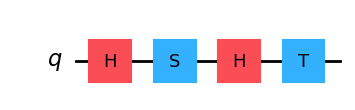
\includegraphics[width=0.4\textwidth]{circuito_thsh.png}
    \caption{El circuito $H\to S\to H\to T$. Se lee de izquierda a derecha, pero su matriz es $THSH$: la primera puerta queda a la derecha del producto.}
    \label{fig:circuito_thsh}
\end{figure}

\noindent La salida obtenida es
\[ \left(\tfrac12 + \tfrac i2\right)|0\rangle + \tfrac{\sqrt2}{2}|1\rangle \]
seguido de
\begin{lstlisting}[language={}]
Coincide con el cálculo a mano: True
Matriz del circuito == T·H·S·H: True
\end{lstlisting}
\noindent es decir, el estado esperado (recordemos que $\frac{\sqrt2}{2} = \frac{1}{\sqrt2}$), y la matriz del circuito es el producto de las puertas \textbf{en orden inverso}.

\subsection{Experimento 2: el circuito de Bell y la convención de orden}

\noindent Aplicamos la Hadamard al qubit de \textbf{arriba} ($q_0$, que es $\mathsf{Y}$) y el CNOT con control $q_0$ y objetivo $q_1$ ($\mathsf{X}$). Según la Sección~3.1, la matriz debe ser $U = \mathrm{CNOT}_{\mathsf{Y}\to\mathsf{X}}\,(\mathbb{I}\otimes H)$ (en el código esta matriz se llama \texttt{CX}, pero no es el $CX$ del Capítulo~2):
\begin{lstlisting}
bell = QuantumCircuit(2)
bell.h(0)
bell.cx(0, 1)

U = Operator.from_circuit(bell).data
print(np.round(sqrt(2) * U, 3).real)

I2 = np.eye(2); Hm = np.array([[1, 1], [1, -1]]) / sqrt(2)
CX = np.array([[1,0,0,0],[0,0,0,1],[0,0,1,0],[0,1,0,0]])
print("U == CX (I ⊗ H):", np.allclose(U, CX @ np.kron(I2, Hm)))

for etiqueta in ["00", "01", "10", "11"]:
    salida = Statevector.from_label(etiqueta).evolve(bell)
    print(f"U|{etiqueta}> =", salida.draw("latex_source"))
\end{lstlisting}

\begin{figure}[htbp]
    \centering
    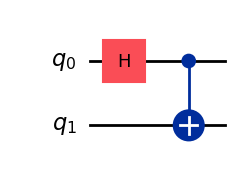
\includegraphics[width=0.3\textwidth]{circuito_bell_cap3.png}
    \caption{Circuito de Bell dibujado por Qiskit: $q_0$ arriba ($\mathsf{Y}$), $q_1$ abajo ($\mathsf{X}$).}
    \label{fig:circuito_bell_cap3}
\end{figure}

\noindent La salida obtenida es
\[ \sqrt2\,U = \begin{pmatrix} 1 & 1 & 0 & 0 \\ 0 & 0 & 1 & -1 \\ 0 & 0 & 1 & 1 \\ 1 & -1 & 0 & 0 \end{pmatrix}, \]
con \texttt{U == CX (I $\otimes$ H): True}, y los cuatro estados de la base se transforman en
\begin{align*}
U|00\rangle &= \tfrac{1}{\sqrt2}|00\rangle + \tfrac{1}{\sqrt2}|11\rangle = |\phi^+\rangle, &
U|01\rangle &= \tfrac{1}{\sqrt2}|00\rangle - \tfrac{1}{\sqrt2}|11\rangle = |\phi^-\rangle, \\
U|10\rangle &= \tfrac{1}{\sqrt2}|01\rangle + \tfrac{1}{\sqrt2}|10\rangle = |\psi^+\rangle, &
U|11\rangle &= -\tfrac{1}{\sqrt2}|01\rangle + \tfrac{1}{\sqrt2}|10\rangle = -|\psi^-\rangle,
\end{align*}
como se calculó a mano en la Sección~3.1. Cada columna de $\sqrt2\,U$ es, salvo el factor, uno de estos estados: la columna $k$ es la imagen del $k$-ésimo vector de la base.

\noindent Obsérvese la diferencia con el Experimento~4 de la Sección~2.3: allí la Hadamard y el control estaban en $q_1$ (el sistema izquierdo, como en las fórmulas del capítulo 2) y el resultado era $|01\rangle\mapsto|\psi^+\rangle$, $|10\rangle\mapsto|\phi^-\rangle$. Aquí están en $q_0$, y los papeles de $|01\rangle$ y $|10\rangle$ se intercambian. Es el mismo circuito ``con los cables cambiados''.

\subsection{Experimento 3: medir el estado de Bell}

\noindent Añadimos una medición a cada qubit y ejecutamos el circuito $1000$ veces:
\begin{lstlisting}
bell_medido = bell.copy()
bell_medido.measure_all()
cuentas = contar(bell_medido, shots=1000)
print(cuentas)
\end{lstlisting}

\begin{figure}[htbp]
    \centering
    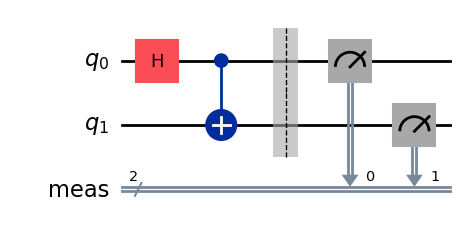
\includegraphics[width=0.42\textwidth]{circuito_bell_medido.png}
    \caption{El circuito de Bell con mediciones. La barrera gris (\textit{barrier}) solo separa visualmente las puertas de las mediciones. Las líneas dobles son bits clásicos: el resultado de medir $q_0$ se guarda en el bit $0$ del registro \texttt{meas}, y el de $q_1$ en el bit $1$.}
    \label{fig:circuito_bell_medido}
\end{figure}

\noindent La salida obtenida es
\begin{lstlisting}[language={}]
{'11': 494, '00': 506}
\end{lstlisting}
\noindent Solo aparecen \texttt{00} y \texttt{11}, cada uno aproximadamente la mitad de las veces: los dos qubits \textbf{siempre coinciden}, aunque cada uno por separado sea completamente aleatorio. La desviación respecto de $500$ es de $6$, muy por debajo del error típico $\sqrt{1000\cdot\frac12\cdot\frac12}\approx 16$ que se vio en la Sección~1.3.

\begin{figure}[htbp]
    \centering
    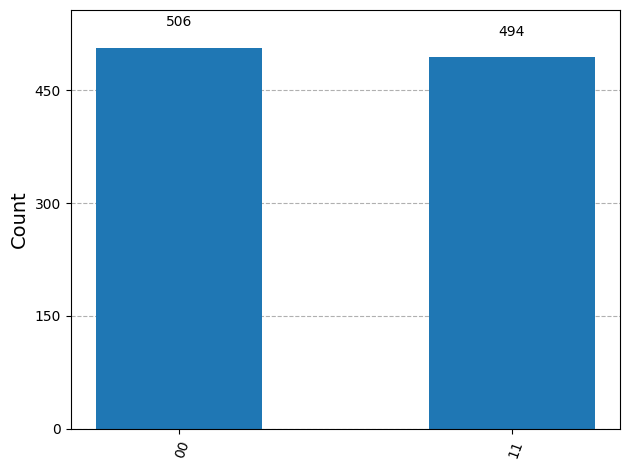
\includegraphics[width=0.5\textwidth]{histograma_bell.png}
    \caption{Resultados de $1000$ mediciones del estado $|\phi^+\rangle$: $506$ veces \texttt{00} y $494$ veces \texttt{11}.}
    \label{fig:histograma_bell}
\end{figure}

\subsection{Experimento 4: productos internos, fidelidad y proyecciones}

\noindent Comprobamos el ejemplo de la Sección~3.2 con $|\psi\rangle = \frac{1+2i}{3}|0\rangle - \frac23|1\rangle$:
\begin{lstlisting}
psi = Statevector([(1 + 2j) / 3, -2 / 3])
mas = Statevector.from_label("+")

# np.vdot conjuga el PRIMER vector, igual que el bra
print("<psi|+> · 3√2 =", np.round(np.vdot(psi.data, mas.data) * 3 * sqrt(2), 6))
print("<+|psi> · 3√2 =", np.round(np.vdot(mas.data, psi.data) * 3 * sqrt(2), 6))

print("Fidelidad |<0|+>|^2 =", round(state_fidelity(Statevector.from_label("0"), mas), 4))
print("Fidelidad |<+|->|^2 =", round(state_fidelity(mas, Statevector.from_label("-")), 4))

P = np.outer(mas.data, mas.data.conj())        # Pi_+ = |+><+|
print("Pi_+ =\n", np.round(P, 3).real)
print("Hermítica:", np.allclose(P, P.conj().T), "   Idempotente:", np.allclose(P @ P, P))
\end{lstlisting}
\noindent La salida obtenida es:
\begin{lstlisting}[language={}]
<psi|+> · 3√2 = (-1-2j)
<+|psi> · 3√2 = (-1+2j)
Fidelidad |<0|+>|^2 = 0.5
Fidelidad |<+|->|^2 = 0.0
Pi_+ =
 [[0.5 0.5]
 [0.5 0.5]]
Hermítica: True    Idempotente: True
\end{lstlisting}
\noindent Es decir, $\langle\psi|+\rangle = \frac{-1-2i}{3\sqrt2}$ y $\langle+|\psi\rangle = \frac{-1+2i}{3\sqrt2}$: al cambiar el orden, el producto interno se \textbf{conjuga}. La fidelidad de $|0\rangle$ con $|+\rangle$ es $\frac12$ y la de $|+\rangle$ con $|-\rangle$ es $0$ (son ortogonales), y
\[ \Pi_+ = |+\rangle\langle+| = \tfrac12\begin{pmatrix} 1 & 1 \\ 1 & 1\end{pmatrix} \]
cumple $\Pi_+^\dagger = \Pi_+$ y $\Pi_+^2 = \Pi_+$, que son las dos condiciones de una proyección.

\subsection{Experimento 5: medir en la base $\{|+\rangle, |-\rangle\}$}

\noindent Según la Sección~3.2, medir en la base $\{|+\rangle,|-\rangle\}$ equivale a aplicar $H$ ($=H^\dagger$) y medir en la base estándar; el resultado $0$ significa ``$+$'' y el $1$ significa ``$-$'':
\begin{lstlisting}
for nombre, preparar in [("|0>", []), ("|+>", ["h"])]:
    qc = QuantumCircuit(1)
    for g in preparar:
        getattr(qc, g)(0)       # preparar el estado
    qc.h(0)                     # cambio a la base {|+>, |->}
    qc.measure_all()
    print(f"Estado {nombre}: {contar(qc)}")
\end{lstlisting}
\noindent La salida obtenida es:
\begin{lstlisting}[language={}]
Estado |0>: {'1': 508, '0': 492}
Estado |+>: {'0': 1000}
\end{lstlisting}
\noindent Para $|0\rangle$ salen ``$+$'' y ``$-$'' mitad y mitad, porque $|\langle+|0\rangle|^2 = |\langle-|0\rangle|^2 = \frac12$. Para $|+\rangle$ sale siempre ``$+$'': es un vector de la base en la que medimos, así que el resultado es seguro.

\subsection{Experimento 6: fase global frente a fase relativa}

\begin{lstlisting}
menos = Statevector.from_label("-")
print("|-> y -|-> iguales salvo fase global:", menos.equiv(Statevector(-menos.data)))
print("|+> y |-> iguales salvo fase global: ", mas.equiv(menos))
print("|<+|->| =", abs(np.vdot(mas.data, menos.data)))
\end{lstlisting}
\noindent La salida obtenida es:
\begin{lstlisting}[language={}]
|-> y -|-> iguales salvo fase global: True
|+> y |-> iguales salvo fase global:  False
|<+|->| = 2.2371143170757382e-17
\end{lstlisting}
\noindent $|-\rangle$ y $-|-\rangle$ son el mismo estado (fase global), mientras que $|+\rangle$ y $|-\rangle$ no lo son: solo se diferencian en una fase \textbf{relativa}, y de hecho son ortogonales. El valor $2.24\cdot10^{-17}$ es un $0$ en coma flotante: el cálculo $\frac12 - \frac12$ se hace con $\frac{1}{\sqrt2}$ redondeado, y queda un residuo del orden de la precisión de la máquina ($\approx 10^{-16}$).

\subsection{Experimento 7: no clonación}

\noindent El candidato a clonador de la Sección~3.3 es el CNOT con control en el qubit a copiar ($q_1$, abajo) y objetivo en el qubit ``en blanco'' ($q_0$, arriba), inicializado en $|0\rangle$:
\begin{lstlisting}
clonador = QuantumCircuit(2)
clonador.cx(1, 0)

for nombre in ["0", "1", "+"]:
    entrada = Statevector.from_label(nombre + "0")        # |psi> ⊗ |0>
    salida = entrada.evolve(clonador)
    deseado = Statevector.from_label(nombre + nombre)     # |psi> ⊗ |psi>
    print(f"|{nombre}>: salida = {salida.draw('latex_source')}  ¿es |{nombre}>|{nombre}>? {salida.equiv(deseado)}")
\end{lstlisting}
\noindent La salida obtenida, resumida en una tabla, es:
\begin{center}
\renewcommand{\arraystretch}{1.3}
\begin{tabular}{c|c|c}
\textbf{Entrada} & \textbf{Salida} & \textbf{¿Es $|\psi\rangle|\psi\rangle$?} \\ \hline
$|0\rangle|0\rangle$ & $|00\rangle$ & \texttt{True} \\
$|1\rangle|0\rangle$ & $|11\rangle$ & \texttt{True} \\
$|+\rangle|0\rangle$ & $\frac{1}{\sqrt2}|00\rangle + \frac{1}{\sqrt2}|11\rangle$ & \texttt{False}
\end{tabular}
\end{center}
\noindent El CNOT copia $|0\rangle$ y $|1\rangle$, pero con $|+\rangle$ no produce $|+\rangle|+\rangle = \frac12(|00\rangle + |01\rangle + |10\rangle + |11\rangle)$, sino el estado entrelazado $|\phi^+\rangle$. Es exactamente el argumento de linealidad del teorema de no clonación: como $|+\rangle = \frac{1}{\sqrt2}(|0\rangle + |1\rangle)$, la salida es la combinación de las copias de $|0\rangle$ y de $|1\rangle$, y eso no es la copia de la combinación.

\subsection{Experimento 8: estimar un kernel cuántico con un circuito}

\noindent Codificamos un dato $x$ con el mapa de características más sencillo posible, una rotación: $|\phi(x)\rangle = R_y(x)|0\rangle$. El kernel exacto es $K(x,y) = |\langle\phi(x)|\phi(y)\rangle|^2 = \cos^2\frac{x-y}{2}$. El circuito $R_y(y)$ seguido de $R_y(x)^\dagger = R_y(-x)$ y una medición da $0$ con probabilidad $K(x,y)$:
\begin{lstlisting}
def kernel_estimado(x, y, shots):
    qc = QuantumCircuit(1)
    qc.ry(y, 0)        # U(y)
    qc.ry(-x, 0)       # U(x)^dagger
    qc.measure_all()
    cuentas = contar(qc, shots)
    return cuentas.get("0", 0) / shots

x, y = 0.3, 1.2
print("Exacto (fórmula):   ", round(np.cos((x - y) / 2) ** 2, 4))
print("Exacto (productos): ", round(kernel_exacto(x, y), 4))
for shots in [100, 1000, 10000]:
    print(f"Estimado con {shots:5d} disparos: {kernel_estimado(x, y, shots):.4f}")
\end{lstlisting}
\noindent donde \texttt{kernel\_exacto} calcula $|\langle\phi(x)|\phi(y)\rangle|^2$ directamente con los vectores de estado. La salida obtenida es:
\begin{lstlisting}[language={}]
Exacto (fórmula):    0.8108
Exacto (productos):  0.8108
Estimado con   100 disparos: 0.8000
Estimado con  1000 disparos: 0.8120
Estimado con 10000 disparos: 0.8118
\end{lstlisting}
\noindent que resumimos en la tabla, junto con el error típico esperado $\sqrt{K(1-K)/N}$:
\begin{center}
\begin{tabular}{r|c|c|c}
\textbf{Disparos} & \textbf{$K$ estimado} & \textbf{Error} $|\hat K - K|$ & \textbf{Error típico} \\ \hline
$100$ & $0.8000$ & $0.0108$ & $0.039$ \\
$1\,000$ & $0.8120$ & $0.0012$ & $0.012$ \\
$10\,000$ & $0.8118$ & $0.0010$ & $0.004$ \\ \hline
exacto & $0.8108$ & &
\end{tabular}
\end{center}
\noindent Todos los errores están por debajo del error típico, que disminuye como $1/\sqrt N$. Las dos formas de calcular el valor exacto coinciden (la fórmula $\cos^2\frac{x-y}{2}$ es correcta), y las estimaciones del circuito se acercan a ese valor al aumentar los disparos, lo que comprueba que el circuito $U(y)$, $U(x)^\dagger$ y medición calcula de verdad el kernel de fidelidad. Es, en miniatura, el procedimiento completo de estimación de un kernel cuántico que se usará en el trabajo: en el TFG, $R_y$ se sustituirá por un mapa de características de varios qubits con entrelazamiento, y habrá que estimar así cada entrada de la matriz $K$.


%=====================================================================
\cleardoublepage
\section{Resumen: un ejemplo guiado}

\noindent Seguimos una sola historia con números: un qubit que pasa por un circuito, se mide de varias formas, y al que intentamos copiar y distinguir.

\paragraph{Parte 1: circuitos}\mbox{}

\pasoguiado{Paso 1. Leer un circuito}
{\begin{quantikz}[column sep=0.25cm] \lstick{$|0\rangle$} & \gate{H} & \gate{S} & \gate{H} & \gate{T} & \end{quantikz}
\quad aplica la matriz $THSH$ y da $\tfrac{1+i}{2}|0\rangle + \tfrac{1}{\sqrt2}|1\rangle$.}
{\textbf{Circuito:} cables = qubits, cajas = puertas (unitarias), de izquierda a derecha y sin ciclos. \textbf{El circuito se lee al revés que la fórmula:} la primera puerta queda a la derecha del producto.}

\pasoguiado{Paso 2. Varios qubits: ¿quién es quién?}
{\begin{quantikz}[row sep=0.2cm,column sep=0.3cm] \lstick{$\mathsf{Y}$} & \gate{H} & \ctrl{1} & \\ \lstick{$\mathsf{X}$} & & \targ{} & \end{quantikz}
\quad $H$ sobre el cable de arriba $= \mathbb{I}\otimes H$ \;(no $H\otimes\mathbb{I}$).}
{\textbf{Convención de Qiskit:} el cable de \textbf{arriba} es $q_0$ = el factor de la \textbf{derecha} del producto tensorial. Leer los cables de abajo arriba = leer la tupla de izquierda a derecha.}

\pasoguiado{Paso 3. Del circuito a la matriz}
{$U = \mathrm{CNOT}_{\mathsf{Y}\to\mathsf{X}}\,(\mathbb{I}\otimes H)$: \quad $U|00\rangle = |\phi^+\rangle$, \; $U|01\rangle = |\phi^-\rangle$, \; $U|10\rangle = |\psi^+\rangle$, \; $U|11\rangle = -|\psi^-\rangle$.}
{Cada ``columna'' de puertas es una matriz; el circuito completo es su producto. Las \textbf{columnas} de $U$ son las imágenes de la base estándar: este circuito fabrica los estados de Bell.}

\pasoguiado{Paso 4. Medir al final del circuito}
{Midiendo los dos qubits de $|\phi^+\rangle$: \texttt{00} o \texttt{11}, cada uno con probabilidad $\frac12$.}
{\textbf{Puerta de medición:} convierte un qubit en un bit clásico (cable doble). El qubit medido se descarta.}

\paragraph{Parte 2: productos internos y proyecciones}\mbox{}

\pasoguiado{Paso 5. Un producto interno}
{$|\psi\rangle = \tfrac{1+2i}{3}|0\rangle - \tfrac23|1\rangle$: \quad $\langle\psi|+\rangle = \tfrac{1-2i}{3\sqrt2} - \tfrac{2}{3\sqrt2} = \tfrac{-1-2i}{3\sqrt2}$, \quad $\langle+|\psi\rangle = \tfrac{-1+2i}{3\sqrt2}$.}
{\textbf{Producto interno} $\langle\psi|\phi\rangle = \sum\overline{\alpha_a}\beta_a$: se \textbf{conjuga el primero}. Al cambiar el orden sale el conjugado. $\langle\psi|\psi\rangle = \|\psi\|^2$.}

\pasoguiado{Paso 6. ¿Cuánto se parecen dos estados?}
{$|\langle0|+\rangle|^2 = \tfrac12$, \qquad $|\langle+|-\rangle|^2 = 0$, \qquad $|\langle-|(-|-\rangle)\rangle|^2 = 1$.}
{\textbf{Cauchy--Schwarz:} para estados, $0\le|\langle\psi|\phi\rangle|^2\le1$ (\textbf{fidelidad}). Vale $1$ si son el mismo estado y $0$ si son \textbf{ortogonales}. El kernel cuántico es una fidelidad.}

\pasoguiado{Paso 7. Una proyección}
{$\Pi_+ = |+\rangle\langle+| = \tfrac12\begin{pmatrix}1&1\\1&1\end{pmatrix}$, \quad $\Pi_+^2 = \Pi_+ = \Pi_+^\dagger$, \quad $\Pi_+|0\rangle = \tfrac{1}{\sqrt2}|+\rangle$, \quad $\Pi_+|-\rangle = 0$.}
{\textbf{Proyección:} hermítica e idempotente; es la ``sombra'' sobre un subespacio. Toda proyección es $\sum_k|\psi_k\rangle\langle\psi_k|$ con $\{|\psi_k\rangle\}$ ortonormal.}

\pasoguiado{Paso 8. Medir en otra base}
{$\{\Pi_+,\Pi_-\}$ sobre $|0\rangle$: \; $\Pr(+) = \|\Pi_+|0\rangle\|^2 = \tfrac12$, \; $\Pr(-) = \tfrac12$. \quad Sobre $|+\rangle$: siempre ``$+$''. \\
En un circuito: \; aplicar $H$ y medir en la base estándar.}
{\textbf{Medición proyectiva:} proyecciones con $\sum_a\Pi_a = \mathbb{I}$; $\Pr(a) = \|\Pi_a|\psi\rangle\|^2$ y el estado pasa a $\Pi_a|\psi\rangle/\|\Pi_a|\psi\rangle\|$. \textbf{Medir en una base} $=$ aplicar $U^\dagger$ (columnas de $U$ = la base) y medir en la base estándar.}

\paragraph{Parte 3: limitaciones}\mbox{}

\pasoguiado{Paso 9. Signos que no importan}
{$|-\rangle$ y $-|-\rangle$: \; $|\langle-|(-|-\rangle)\rangle| = 1$ \; (el mismo estado). \qquad $|+\rangle$ y $|-\rangle$: \; $|\langle+|-\rangle| = 0$ \; (distintos).}
{\textbf{Fase global:} ninguna operación ni medición la detecta, así que es el mismo estado. \textbf{Fase relativa:} cambia el estado. Se reconoce con $|\langle\psi|\phi\rangle| = 1$.}

\pasoguiado{Paso 10. Intentar copiar con un CNOT}
{$\mathrm{CNOT}\,|0\rangle|0\rangle = |00\rangle$ \checkmark, \quad $\mathrm{CNOT}\,|1\rangle|0\rangle = |11\rangle$ \checkmark, \quad pero
\[ \mathrm{CNOT}\,|+\rangle|0\rangle = \tfrac{1}{\sqrt2}(|00\rangle + |11\rangle) \;\neq\; |+\rangle|+\rangle = \tfrac12(|00\rangle + |01\rangle + |10\rangle + |11\rangle). \]}
{\textbf{Teorema de no clonación:} ninguna unitaria copia todos los estados, porque copiar ($|\psi\rangle\mapsto|\psi\rangle|\psi\rangle$) no es lineal. Solo se pueden copiar estados \textbf{ortogonales entre sí}, como $|0\rangle$ y $|1\rangle$.}

\pasoguiado{Paso 11. Intentar distinguir}
{$|+\rangle$ frente a $|-\rangle$ ($\langle+|-\rangle = 0$): \; $H$ y medir, sin error. \qquad $|0\rangle$ frente a $|+\rangle$ ($\langle0|+\rangle = \frac{1}{\sqrt2}\neq0$): imposible sin error.}
{\textbf{Discriminación perfecta} $\iff$ \textbf{ortogonalidad}. El producto interno mide lo distinguibles que son dos estados.}

\begin{center}
\small\renewcommand{\arraystretch}{1.15}
\begin{tabular}{c|l|l}
\textbf{Paso} & \textbf{Qué hicimos} & \textbf{Concepto} \\ \hline
1 & $H\to S\to H\to T$ & Circuito; se lee al revés que la fórmula \\
2 & Hadamard arriba & Convención de orden de Qiskit \\
3 & $U = \mathrm{CNOT}_{\mathsf{Y}\to\mathsf{X}}(\mathbb{I}\otimes H)$ & Del circuito a la matriz; estados de Bell \\
4 & Medir $|\phi^+\rangle$ & Puertas de medición y bits clásicos \\
5 & $\langle\psi|+\rangle$ & Producto interno (conjugar el primero) \\
6 & $|\langle0|+\rangle|^2 = \frac12$ & Cauchy--Schwarz, fidelidad, ortogonalidad \\
7 & $\Pi_+$ & Proyección \\
8 & $H$ y medir & Medición proyectiva; medir en otra base \\
9 & $-|-\rangle$ & Fase global frente a fase relativa \\
10 & CNOT sobre $|+\rangle$ & No clonación \\
11 & $|0\rangle$ frente a $|+\rangle$ & Discriminación $\iff$ ortogonalidad
\end{tabular}
\end{center}

\noindent \textbf{Conexión con el TFG:} el kernel cuántico reúne todo el capítulo. Se \textbf{estima con un circuito} ($U(\mathbf{y})$, $U(\mathbf{x})^\dagger$ y medir, pasos 1--4); su valor es una \textbf{fidelidad} entre $0$ y $1$ (paso 6); es la probabilidad de un resultado de una \textbf{medición proyectiva} (paso 8); no depende de \textbf{fases globales} (paso 9); y mide \textbf{lo distinguibles} que son los estados de dos datos (paso 11).



% ========================= BIBLIOGRAFÍA =============================
\cleardoublepage
\begin{thebibliography}{9}

\bibitem{watrous2024understanding}
J.~Watrous.
\newblock \emph{Understanding Quantum Information and Computation}.
\newblock IBM Quantum Learning.
\newblock \url{https://quantum.cloud.ibm.com/learning}

\bibitem{havlicek2019supervised}
V.~Havlíček, A.~D.~Córcoles, K.~Temme, A.~W.~Harrow, A.~Kandala, J.~M.~Chow y J.~M.~Gambetta.
\newblock Supervised learning with quantum-enhanced feature spaces.
\newblock \emph{Nature}, 567:209--212, 2019.

\bibitem{thanasilp2024exponential}
S.~Thanasilp, S.~Wang, M.~Cerezo y Z.~Holmes.
\newblock Exponential concentration in quantum kernel methods.
\newblock \emph{Nature Communications}, 15:5200, 2024.

\end{thebibliography}

\end{document}
